% Here you can input the chapters into the project
% \chapter{Introduction}
% \input{chapters/01-introduction.tex}
\section{Data Introduction}
In this section we will explore the dataset from HOME that is to be analysed in this project.
The dataset consists of information regarding property sales in the period from 2004 to 2016.
It has 131.920 observations where the price as well as some additional information on the property in question has been recorded.
Following a preliminary examination of the dataset, we have chosen to focus on apartments in the four largest danish cities. 
These being Copenhagen, Aarhus, Odense and Aalborg.
For the variables we have chosen to focus on
%\begin{multicols}{2}
\begin{enumerate}
    \item City
    \item Property Condition
    % \begin{itemize}[label = -]
    %     \item A qualitative evaluation of the condition of the property which can fall in one of three categories; ``Bad'', ``Okay'', ``Good''.
    % \end{itemize}
    \item Size in $m^2$
    % \begin{itemize}[label = -]
    %     \item The number of square meters that represents actual living space whitin the property. 
    % \end{itemize}
    \item Year of sale
    \item Selling period in days
    % \begin{itemize}[label = -]
    %     \item Number of days between the day the property went on the market and the day the property was sold.
    % \end{itemize}
    \item Year of construction
    \item Balcony or not
    % \begin{itemize}[label = -]
    %     \item A binary variable that tells whether or not the property have a balcony.
    % \end{itemize}
    \item Renovation or not
    % \begin{itemize}[label = -]
    %     \item A binary variable that tells if the property have ever been renovated.
    % \end{itemize}
\end{enumerate}
%\end{multicols}
Restricting to the cities in question results in a reduction of the number of observations.
Furthermore we have chosen to disregard observations that contain NA values.
The number of observations after the reduction is 3.086.

\section{Partitioning the Dataset}
In preparation for section \ref{sec:prediction} we will set aside the observations from sales in 2016.
These observations can then be used to asses the predictive accuracy of the models that will be developed in the project.
The number of sales in 2016 amounts to 200 observations, the distribution between cities can be found in table \ref{tbl:2016_obs_per_city}.
\begin{table}[H]
    \centering
    \begin{tabular}{lr}
        \toprule
        \textbf{City} & \textbf{Obs.}\\
        \midrule
        Copenhagen & 108\\
        Odense & 27\\
        Aalborg & 19\\
        Aarhus & 46\\
        \bottomrule
    \end{tabular}
    \caption{Count of apartments sold in 2016 per city.}
    \label{tbl:2016_obs_per_city}
\end{table}
In the next section we will investigate the remaining observations from the dataset, i.e. the observations that were sold between 2004 and 2016.

\section{Descriptive Statistics}
This section will provide a brief summary for each of the variables.
But first we can take a look at the price which will be treated as the dependent variable in this project.
In table \ref{tbl:summary_of_price} a summary of the apartment prices can be seen.
In table \ref{tbl:summary_of_price}, \textbf{Q1} and \textbf{Q3} represents the first and third quartile respectively.
\begin{table}[H]
    \centering
    \begin{tabular}{rrrrrrr}
        \toprule
        \textbf{minimum} & \textbf{Q1} & \textbf{median} & \textbf{mean} & \textbf{Q3} & \textbf{maximum} & \textbf{std. deviation}\\
        \midrule
        200\:000 & 1\:175\:000 & 1\:725\:000 & 2\:069\:337 & 2\:600\:000 & 15\:550\:000 & 1\:302\:274\\
        \bottomrule
    \end{tabular}
    \caption{Summary of apartment prices.}
    \label{tbl:summary_of_price}
\end{table}
To further investigate the distribution of the price a histogram of the apartment prices has been plotted in figure \ref{fig:histogram_of_price}.
As is evident on the plot, the price is clearly left skewed.
This is expected as the median is below the mean.
\begin{figure}[H]
    \centering
    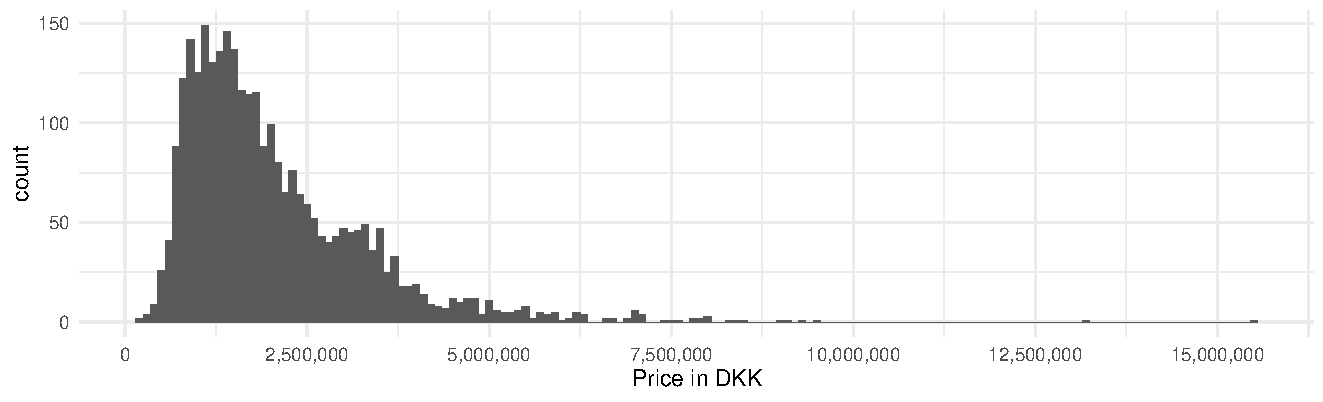
\includegraphics[width=0.9\textwidth]{figures/Data_introduction/price_histogram.pdf}
    \caption{A histogram of the apartment price with a binwidth of 100\:000 DKK.}
    \label{fig:histogram_of_price}
\end{figure}

\subsection*{City}
How the observations are distributed between the cities can be seen on figure \ref{fig:distributions_between_cities}.
\begin{figure}[H]
    \centering
    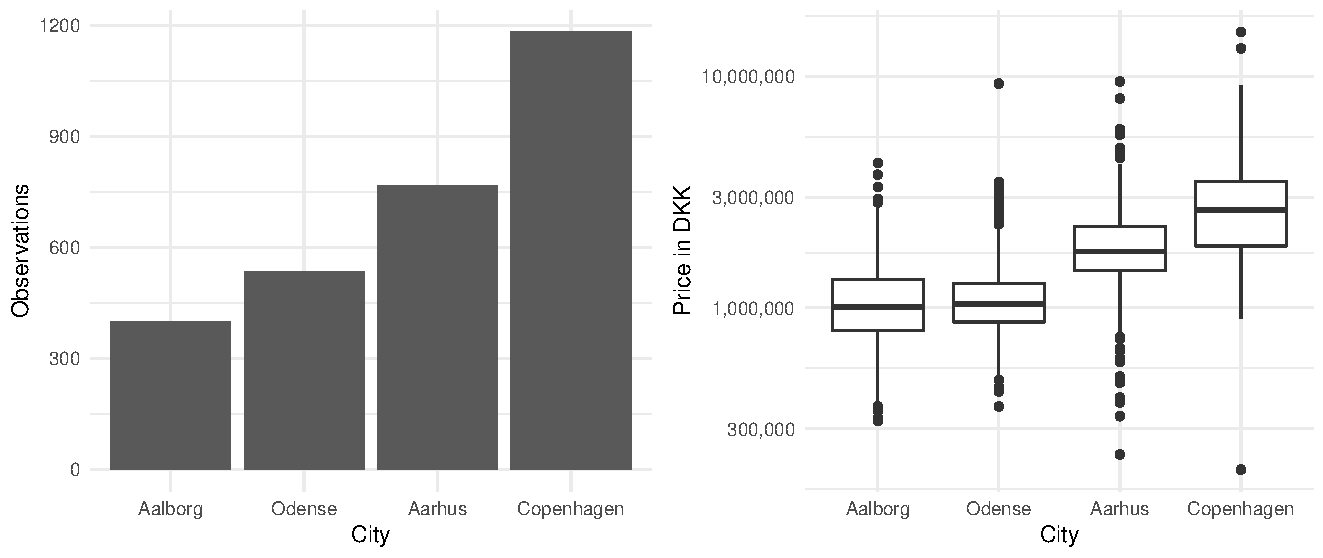
\includegraphics[width=0.9\textwidth]{figures/Data_introduction/distribution_between_cities.pdf}
    \caption{Distribution of observations and a boxplot of price between the cities.}
    \label{fig:distributions_between_cities}
\end{figure}
Here it is seen that most observations are from Copenhagen, which is to be expected as there are more apartments than in the other 3 cities.
The differences in the average price between the cities indicate that, this may influence the selling price.

\subsection*{Quality of property}
A qualitative evaluation of the condition of the property which can fall in one of three categories; ``Low'', ``Medium'', ``High''.
A count of the 2.886 total observations in each of the categories can be found in table \ref{tbl:property_condition}.
\begin{table}[H]
    \centering
    \begin{tabular}{lr}
        \toprule
        \textbf{Property Condition} & \textbf{Obs.}\\
        \midrule
        Low & 86\\
        Medium & 1472\\
        High & 1328\\
        \bottomrule
    \end{tabular}
    \caption{Count of observations per property condition.}
    \label{tbl:property_condition}
\end{table}
It is notable that there are very few observations in the ``Low'' category, compared to the other two. 
This variable may not prove very useful since every category is so large.

\subsection*{Size in \textit{m}$\mathbf{^2}$}
This variable measures the size of the property in square meters.
\begin{table}[H]
    \centering
    \begin{tabular}{rrrrrrr}
        \toprule
        \textbf{minimum} & \textbf{Q1} & \textbf{median} & \textbf{mean} & \textbf{Q3} & \textbf{maximum} & \textbf{std. deviation}\\
        \midrule
        12 & 59 & 75 & 81.42238 & 94 & 438 & 33.30229\\
        \bottomrule
    \end{tabular}
    \caption{Summary of the ``size in $m^2$'' variable.}
    \label{tbl:size_in_m2}
\end{table}
A widely used measure for the price of a house is the price per square meter.
In figure \ref{fig:price_per_square_meter} the relationship between the selling price and size of apartments is illustrated.
The figure shows a clear positive relationship between the two variables in all of the four cities.
\begin{figure}[H]
    \centering
    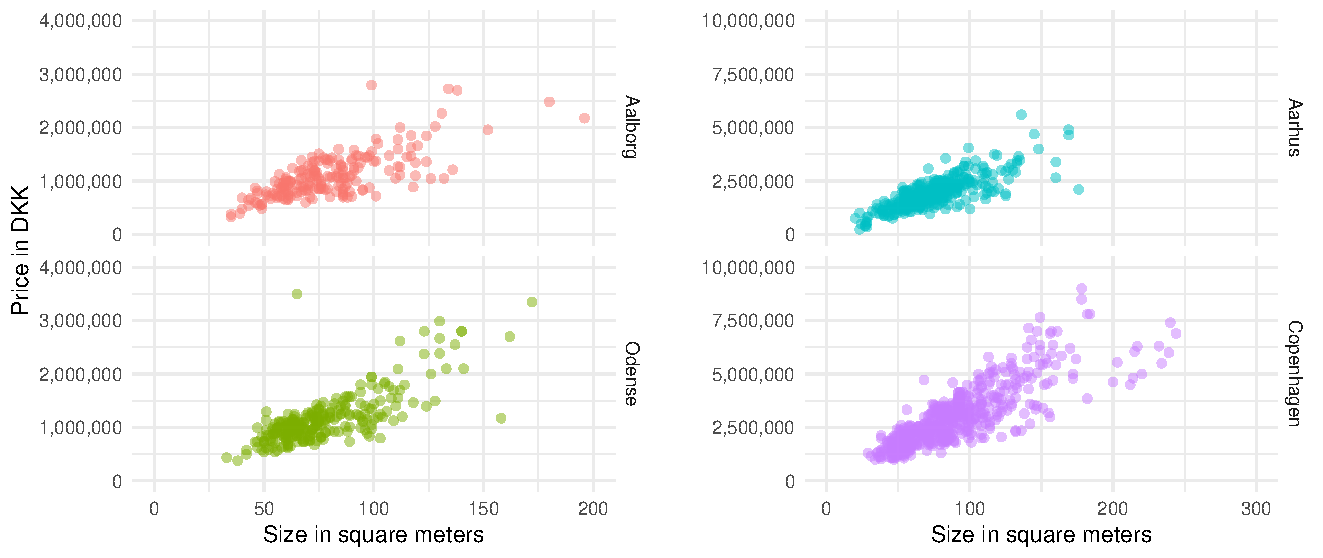
\includegraphics[width=\textwidth]{figures/Data_introduction/price_per_square_meter.pdf}
    \caption{Relationship between the selling price and size of apartments in the four cities.}
    \label{fig:price_per_square_meter}
\end{figure}

\subsection*{Year of Sale}
This variable is a categorical variable that can take one of three possible outcomes, namely ``pre.crisis'', ``crisis'' or ``post.crisis''.
In table \ref{tbl:year_of_sale} a count of observations in each of the categories can be found.
\begin{table}[H]
    \centering
    \begin{tabular}{lr}
        \toprule
        \textbf{Year of Sale} & \textbf{Obs.}\\
        \midrule
        pre.crisis & 1008\\
        crisis & 1001\\
        post.crisis & 877\\
        \bottomrule
    \end{tabular}
    \caption{Count of observations per year of sale category.}
    \label{tbl:year_of_sale}
\end{table}

In figure \ref{fig:year_of_sale_histogram} it can be seen how the distribution of sales have been in the period from 2004 to 2016.
\begin{figure}[H]
    \centering
    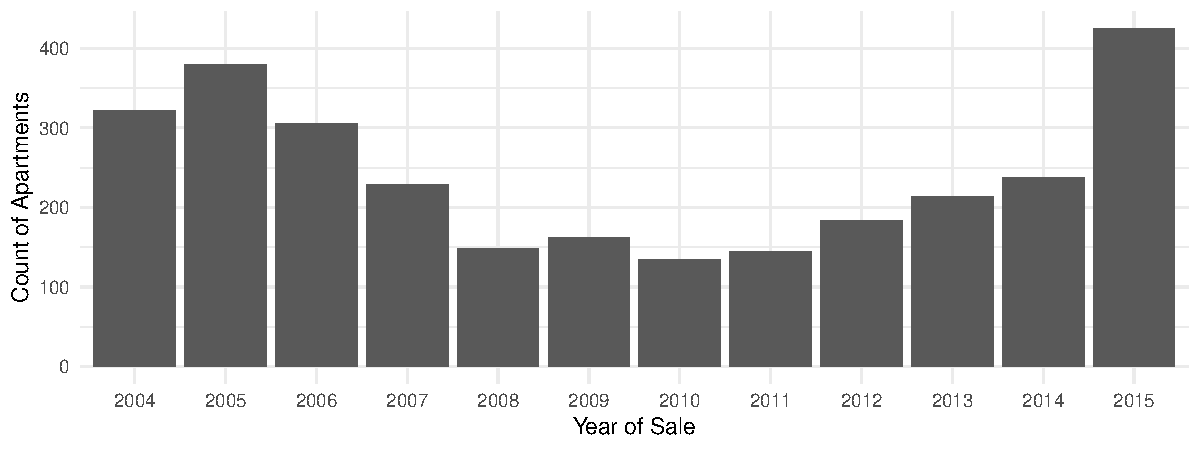
\includegraphics[width = 0.8 \textwidth]{figures/Data_introduction/year_of_sale_histogram.pdf}
    \caption{Histogram showing how many sales there have been per year.}
    \label{fig:year_of_sale_histogram}
\end{figure}
% \begin{table}[H]
%     \centering
%     \begin{tabular}{lr|lr|lr}
%         \toprule
%         \multicolumn{2}{c}{\textbf{2004-2008}} & \multicolumn{2}{c}{\textbf{2009-2013}} &
%         \multicolumn{2}{c}{\textbf{2014-2015}} \\
%         \toprule
%         \textbf{Year of sale} & \textbf{Obs.} & 
%         \textbf{Year of sale} & \textbf{Obs.} & 
%         \textbf{Year of sale} & \textbf{Obs.}\\
%         \midrule
%         2004 & 322 & 2009 & 162 & 2014 & 238\\   
%         2005 & 380 & 2010 & 134 & 2015 & 425\\   
%         2006 & 306 & 2011 & 144\\   
%         2007 & 229 & 2012 & 184\\   
%         2008 & 148 & 2013 & 214\\   
%         \bottomrule
%     \end{tabular}
%     \caption{Summary of the ``Year of sale'' variable.}
%     \label{tbl:year_of_sale}
% \end{table}
As mentioned the dataset includes house sales in the period from 2004 to 2016.
Naturally there will be some fluctuations in the average price from one year to another, just as a result of the economic cycle.
Especially the years during the financial crisis a fall in the average selling price is expected.
Indeed it is also possible to see this trend in the data as figure \ref{fig:house_price_year} suggest.

\subsection*{Selling Period}
This is a variable that counts the number of days it took to sell the apartment.
If the value is 0 the apartment was either sold the day it went on the market or it might not even have been on the market.
\begin{table}[H]
    \centering
    \begin{tabular}{rrrrrrr}
        \toprule
        \textbf{minimum} & \textbf{Q1} & \textbf{median} & \textbf{mean} & \textbf{Q3} & \textbf{maximum} & \textbf{std. deviation}\\
        \midrule
        0 & 27 & 62.5 & 97.7079 & 131.75 & 1321 & 112.5781\\
        \bottomrule
    \end{tabular}
    \caption{Days until the property was sold.}
    \label{tbl:days_until_sold}
\end{table}

\subsection*{Decade of Construction}
The dataset has information regarding which year the apartment have been constructed.
We have here chosen to group the variable in decades.
In table \ref{tbl:year_of_constuction} there is a count of apartments constructed per decade.
\begin{table}[H]
    \centering
    \begin{tabular}{lr|lr|lr|lr|lr}
        \toprule [1.5pt]
        \multicolumn{2}{c}{\textbf{1800-1840}} & 
        \multicolumn{2}{c}{\textbf{1850-1890}} & 
        \multicolumn{2}{c}{\textbf{1900-1940}} & 
        \multicolumn{2}{c}{\textbf{1940-1990}} & 
        \multicolumn{2}{c}{\textbf{2000-2010}} \\[2pt]
        \toprule[1.5pt]
        \textbf{Year} & \textbf{Obs.} & 
        \textbf{Year} & \textbf{Obs.} & 
        \textbf{Year} & \textbf{Obs.} & 
        \textbf{Year} & \textbf{Obs.} & 
        \textbf{Year} & \textbf{Obs.} \\
        \midrule
        1800 & 88 & 1850 & 46  & 1900 & 305 & 1950 & 231 & 2000 & 145 \\
        1810 & 20 & 1860 & 28  & 1910 & 163 & 1960 & 166 & 2010 & 160 \\
        1820 & 6  & 1870 & 89  & 1920 & 144 & 1970 & 74  \\
        1830 & 14 & 1880 & 164 & 1930 & 585 & 1980 & 71  \\
        1840 & 39 & 1890 & 227 & 1940 & 97  & 1990 & 24  \\
        \bottomrule
    \end{tabular}
    \caption{Count of observation per decade of construction}
    \label{tbl:year_of_constuction}
\end{table}
An interesting pattern in the data is how the selling price is affected by the year of construction.
A possible intuition would be that the newer the apartment the higher the selling price, however the data suggests another pattern as is evident in figure \ref{fig:house_price_year}.

\begin{figure}[H]
    \centering
    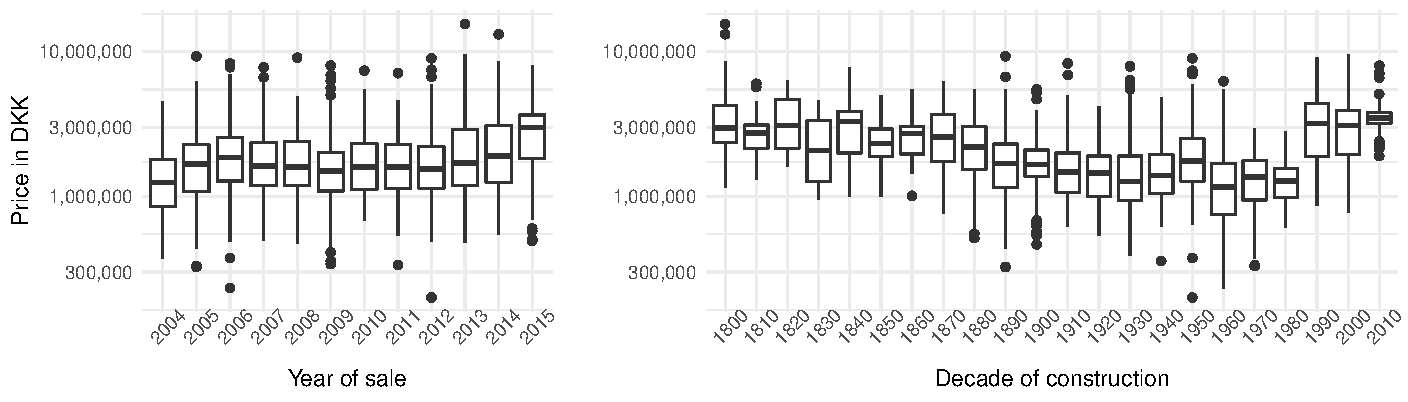
\includegraphics[width = \textwidth]{figures/Data_introduction/house_price_year.pdf}
    \caption{A boxplot of the average selling price against the year of sale and the decade of construction respectively.}
    \label{fig:house_price_year}
\end{figure}
The pattern suggested is that new apartments as well as old apartment have the highest mean price, whereas the apartments constructed from the 1890's until the 1980's have a lower mean price.
However there could be other factors to account for.

\subsection*{Balcony and Renovation}
The variables regarding whether the apartment has a balcony or has been renovated are binary.
This means that they can take either the value 0 or 1, where 0 refers to the case where the apartment does not have a balcony or has not been renovated and vice versa.
\begin{table}[H]
    \centering
    \begin{tabular}{lr}
        \toprule
        \textbf{Balcony or not} & \textbf{Obs.}\\
        \midrule
        0 & 1508\\
        1 & 1378\\
        \bottomrule
    \end{tabular}
    \hspace{20pt}
    \begin{tabular}{lr}
        \toprule
        \textbf{Renovation or not} & \textbf{Obs.}\\
        \midrule
        0 & 2329\\
        1 & 557\\
        \bottomrule
    \end{tabular}
    \caption{Count of observations per balcony and renovation.}
\end{table}

%How the observations are distributed between the cities can be seen %on figure \ref{fig:distributions_between_cities}.
%\begin{figure}[H]
%    \centering
%    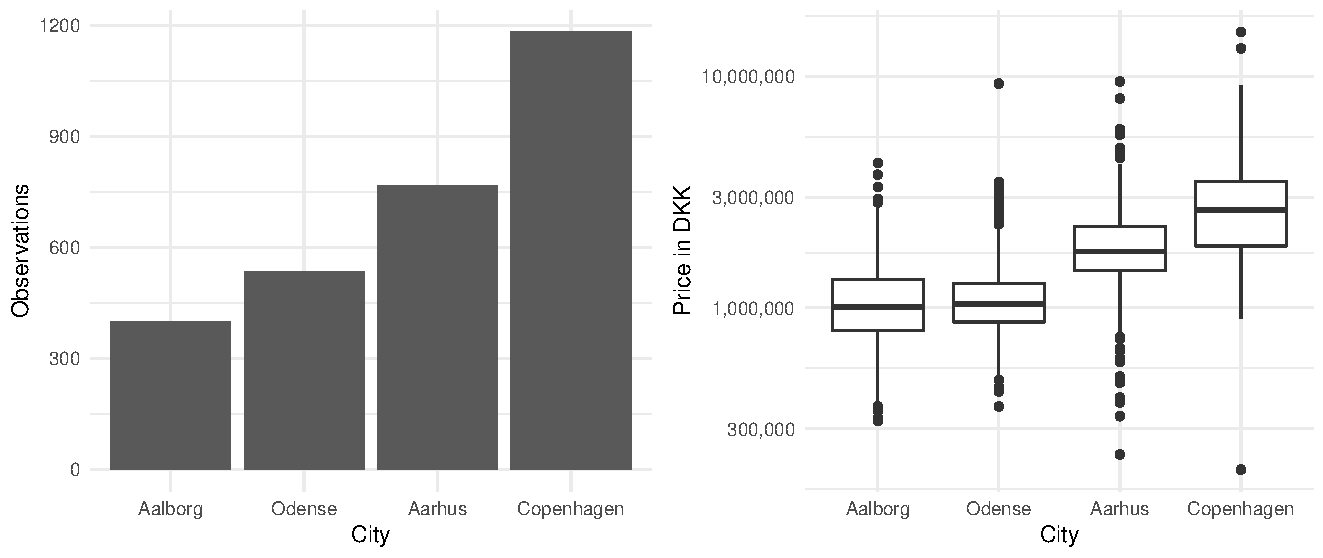
\includegraphics[width=0.9\textwidth]{figures/Data_introduction/distribution_between_cities.pdf}
%    \caption{Distribution of observations and a boxplot of price between the cities.}
%    \label{fig:distributions_between_cities}
%\end{figure}
%
%Here it is seen that most observations are from Copenhagen, which is %to be expected as there are more property than in the other 3 cities.
%We can also note the differences in the average price between the %cities indicating that, all else equal just knowing the city in which %the apartment is located tells something about its price.

%Another widely used measure of the price of a house is the price per %square meter.
%In figure \ref{fig:price_per_square_meter} the relationship between %the selling price and size of apartments is illustrated.
%The figure shows a clear positive relationship between the two %variables in all of the four cities.
%\begin{figure}[H]
%    \centering
%    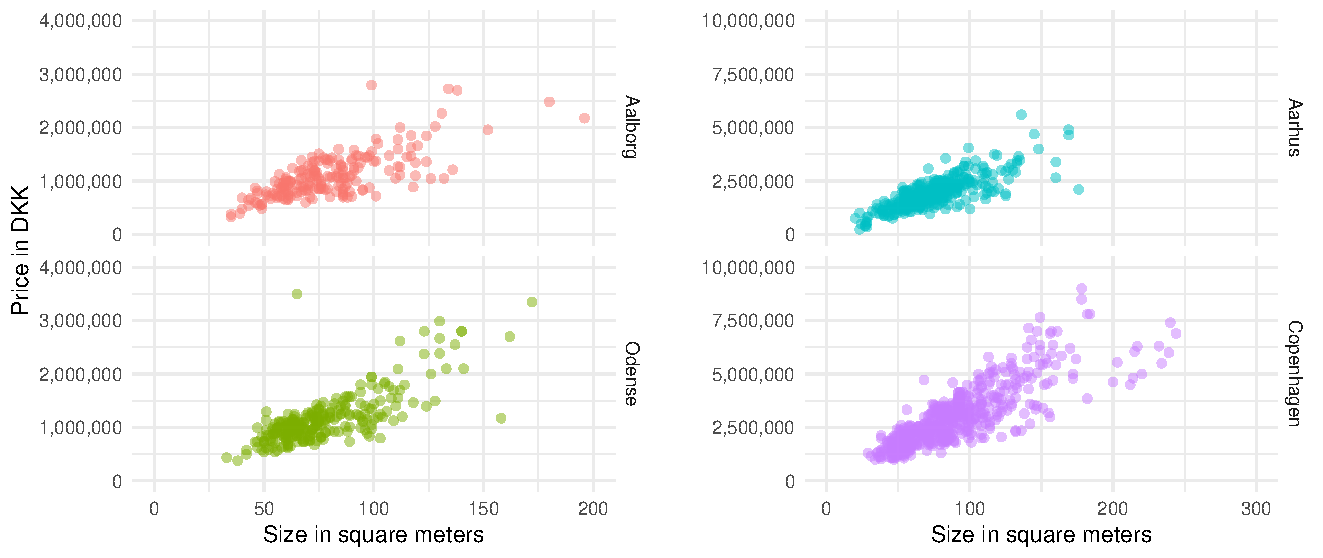
\includegraphics[width=\textwidth]{figures/Data_introduction/price_per_square_meter.pdf}
%    \caption{Relationship between the selling price and size of apartments in the four cities.}
%    \label{fig:price_per_square_meter}
%\end{figure}
%As mentioned the data set includes house sales in the period from %2004 to 2016.
%Naturally there will be some fluctuations in the average price from %one year to another, just as a result of the economic cycle.
%Especially the years during the housing crisis a fall in the average %selling price is expected.
%Indeed it is also possible to see this trend in the data as figure %\ref{fig:house_price_year} suggest.
\chapter{Likelihood Theory}
\label{ch:likelihood_theory}
The aim of this chapter is to present some of the key results from likelihood theory. 
The purpose of likelihood theory is to find the parameters in a given statistical model, which is most compatible with observed data. 
Through maximum likelihood estimation one obtains the estimates of the parameters in a statistical model, which maximises the likelihood function. 
This parameterization of the distribution has most likely generated the data.

\section{Estimation Theory}

First some general terminology and results regarding statistical inference will be introduced.

\begin{definition} [Estimate and Estimator]
    A function $\boldsymbol{\hat{\beta}}$ of a random variable, $\textbf{Y}$, that is used to estimate unknown parameters $\boldsymbol{\beta}$, is called an estimator of $\boldsymbol{\beta}$. The observed value of $\boldsymbol{\hat{\beta}}$ is called the estimate of $\boldsymbol{\beta}$.
\end{definition}

This estimator have the following properties. 

\begin{definition}[Unbiased Estimator]
\label{def:Unbiased_estmator}
Any estimator $\boldsymbol{\hat{\beta}} = \boldsymbol{\hat{\beta}}(Y)$ is said to be unbiased if $E[\boldsymbol{\hat{\beta}}] = \boldsymbol{\beta}, \ \forall \boldsymbol{\beta} \in \Theta^k$,
\end{definition}

where $\Theta^k$ is the parameter space. This means, that an estimator is considered unbiased, if the mean is equal to the true parameter value. 
In other words, the estimator neither overestimates or underestimates.

\begin{definition} [Consistent Estimator]
\label{def:consistent_estimator}
An estimator is consistent if the sequence $\betahat_n(\textbf{Y})$ of estimators for all $\boldsymbol{\beta} \in \Theta^k$ and $\varepsilon > 0$ satisfies,
\begin{align*}
    P_{\boldsymbol{\beta}}(||\hat{\boldsymbol{\beta}}_n(\textbf{Y}) - \boldsymbol{\beta}|| > \varepsilon) \xrightarrow[n \rightarrow \infty]{P} 0.
\end{align*}
Otherwise the estimator is said to be inconsistent.
\end{definition}

This means that the parameter is said to be consistent if the estimate converges in probability towards the true value. 
The desired estimator is often the one with least variance, since we want a parameter close to the expected value. The formal condition for this is given in the following definition.

\begin{definition} [Uniformly Minimum Mean Square Error]
\label{def:minimum_mean_square_error}
An estimator $\boldsymbol{\hat{\beta}}=\boldsymbol{\hat{\beta}}(\textbf{Y})$ is said to be a \textit{uniformly minimum square error estimator}, if
\begin{align*}
    \var(\boldsymbol{\hat{\beta}}(\textbf{Y})) = E\big[ (\boldsymbol{\hat{\beta}}(\textbf{Y})-\boldsymbol{\beta})(\boldsymbol{\hat{\beta}}(\textbf{Y})-\boldsymbol{\beta})^T \big] \leq E\big[ (\boldsymbol{\tilde{\beta}}(\textbf{Y})-\boldsymbol{\beta})(\boldsymbol{\tilde{\beta}}(\textbf{Y})-\boldsymbol{\beta})^T \big] = \var(\boldsymbol{\tilde{\beta}}(Y))
\end{align*} 
for all $\boldsymbol{\beta} \in \Theta^k $ and all other estimators $\boldsymbol{\tilde{\beta}(\textbf{Y})}$.
 \end{definition}
 
If a minimum mean square estimator is considered a linear function of data, it is the best linear unbiased estimator (BLUE).

As mentioned a low variance is often desired and a way to determine the lower bound of an unbiased estimators variance is the Cramer-Rao inequality.
 
 \begin{theorem} [Cramer-Rao Inequality]
\label{th:cramerrao_inequality}
Given the paramtetric density $f_{\textbf{Y}}(\textbf{y};\boldsymbol{\beta}), \ \boldsymbol{\beta} \in \Theta^k$ for the observations $\textbf{Y}$ and assuming that $\textit{\textbf{i}}(\boldsymbol{\beta})$ is invertible for all $\boldsymbol{\beta} \in \Theta^k$ and interchanging of the derivative and integral is allowed, the covariance matrix of any unbiased estimator $\boldsymbol{\hat{\beta}}(\textbf{Y})$ of $\boldsymbol{\beta}$ satisfies the inequality
\begin{align} \label{eq:cramerrao_inequality}
    \var \Big[ \boldsymbol{\hat{\beta}}(\textbf{Y})\Big] \geq \textit{\textbf{i}}^{-1}(\boldsymbol{\beta})
\end{align}
where $\textit{i}(\beta)$ is the \textit{Fisher information matrix} which is defined as
\begin{align*}
    \textit{\textbf{i}}(\boldsymbol{\beta})=E \bigg[ \bigg(\frac{\partial \log f_Y(\textbf{Y};\boldsymbol{\beta})}{\partial \boldsymbol{\beta}} \bigg)\bigg(\frac{\partial \log f_Y(\textbf{Y};\boldsymbol{\beta})}{\partial \boldsymbol{\beta}}\bigg)^\top\bigg]
\end{align*}
where $\var [\boldsymbol{\hat{\beta}}(\textbf{Y})]=E[(\boldsymbol{\hat{\beta}}(\textbf{Y})-\boldsymbol{\beta})(\boldsymbol{\hat{\beta}}(\textbf{Y})-\boldsymbol{\beta})^\top]$.
\end{theorem}

Note that the inequality in \eqref{eq:cramerrao_inequality} entails that the right hand side subtracted from the left hand side is positive semidefinite.

\begin{proof}
First, we see that
\begin{align*}
    E\Big[\boldsymbol{\hat{\beta}}(\textbf{Y}) \frac{\partial \log f_Y(\textbf{Y};\boldsymbol{\beta})}{\partial \boldsymbol{\beta}} \Big]
    &=\int \boldsymbol{\hat{\beta}}(\textbf{y})\frac{\partial \log f_Y(\textbf{y};\boldsymbol{\beta})}{\partial \boldsymbol{\beta}}f_Y(\textbf{y};\boldsymbol{\beta}) \text{dy} \\
    &= \int \boldsymbol{\hat{\beta}}(\textbf{y})\frac{1}{f_Y(\textbf{y};\boldsymbol{\beta})}\frac{\partial f_Y(\textbf{y};\boldsymbol{\beta})}{\partial \boldsymbol{\beta}}f_Y(\textbf{y};\boldsymbol{\beta}) \text{dy} \\
    &=\int \boldsymbol{\hat{\beta}}(\textbf{y}) \frac{\partial}{\partial \boldsymbol{\beta}}f_Y(\textbf{y};\boldsymbol{\beta}) \text{dy} \\
    &=\frac{\partial}{\partial \boldsymbol{\beta}} \int \boldsymbol{\hat{\beta}}(\textbf{y}) f_Y(\textbf{y};\boldsymbol{\beta}) \text{dy}
\end{align*}
where we obtain the latter from the regularity conditions. 
Since $\boldsymbol{\hat{\beta}}(\textbf{Y})$ is unbiased, c.f. definition \ref{def:Unbiased_estmator}, we see that
\begin{align}
    \frac{\partial}{\partial \boldsymbol{\beta}} \int \boldsymbol{\hat{\beta}}(\textbf{y}) f_Y(\textbf{y};\boldsymbol{\beta}) \text{dy} &= \frac{\partial}{\partial\boldsymbol{\beta}} E\big[ \boldsymbol{\hat{\beta}}(\textbf{Y})\big] \nonumber\\
    &= \frac{\partial}{\partial\boldsymbol{\beta}} \boldsymbol{\beta} \nonumber\\
    &= I_{k} \label{eq:cramerraoe2stjerner}.
\end{align}
Furthermore, we see that
\begin{align}
    E\Big[ \frac{\partial \log f_Y(\textbf{Y};\boldsymbol{\beta})}{\partial \boldsymbol{\beta}}\Big] &= \int \frac{\partial \log f_Y(\textbf{y};\boldsymbol{\beta})}{\partial \boldsymbol{\beta}}f_Y(\textbf{y};\boldsymbol{\beta}) \text{dy} \nonumber \\
    &=\int  \frac{\partial}{\partial \boldsymbol{\beta}}f_Y(\textbf{y};\boldsymbol{\beta}) \text{dy} \nonumber \\
    &=\frac{\partial}{\partial \boldsymbol{\beta}} \int f_Y(\textbf{y};\boldsymbol{\beta}) \text{dy} \nonumber \\
    &= \textbf{0}_{1 \times k} \label{eq:cramerraoe3stjerner}.
\end{align}
We are now able to find the covariance matrix for $\begin{bmatrix} \boldsymbol{\hat{\beta}}(\textbf{Y}) & \partial \log f_Y(\textbf{Y};\boldsymbol{\beta})/\partial \boldsymbol{\beta}) \end{bmatrix}^T$
\begin{align*}
    \var \begin{bmatrix}  \boldsymbol{\hat{\beta}}(\textbf{Y}) \\  \partial \log f_Y(\textbf{Y};\boldsymbol{\beta})/\partial \boldsymbol{\beta}) \end{bmatrix} &= E \begin{bmatrix} \begin{pmatrix} \boldsymbol{\hat{\beta}}(\textbf{Y})-\boldsymbol{\beta} \\  \partial \log f_Y(\textbf{Y};\boldsymbol{\beta})/\partial \boldsymbol{\beta})^T\end{pmatrix} \begin{pmatrix} \boldsymbol{\hat{\beta}}(\textbf{Y}-\boldsymbol{\beta})^T &  \partial \log f_Y(\textbf{Y};\boldsymbol{\beta})/\partial \boldsymbol{\beta} \end{pmatrix}\end{bmatrix}  \\
    &= \var \begin{bmatrix} \boldsymbol{\hat{\beta}}(\textbf{Y}) & I_{k}\\
    I_{k} & \textbf{i}(\boldsymbol{\beta})\end{bmatrix}.
\end{align*}
Because of symmetry in \eqref{eq:cramerraoe2stjerner} and \eqref{eq:cramerraoe3stjerner} the covariance matrix is clearly positive semidefinite, and we have
\begin{align*}
    0_{k} & \leq \begin{bmatrix} I_{k} & -\textbf{i}^{-1}(\boldsymbol{\beta})\end{bmatrix} \begin{bmatrix} \var[\boldsymbol{\hat{\beta}}(\textbf{Y})] & I_{k} \\ I_{k} & \textbf{i}(\boldsymbol{\beta}) \end{bmatrix}\begin{bmatrix} I_{k} \\ -\textbf{i}^{-1}(\boldsymbol{\beta})\end{bmatrix} \\
    &= \begin{bmatrix} \var[\boldsymbol{\hat{\beta}}(\textbf{Y})] -\textbf{i}^{-1}(\boldsymbol{\beta}) & 0_{k}\end{bmatrix} \begin{bmatrix} I_{k} \\ -\textbf{i}^{-1}(\boldsymbol{\beta})\end{bmatrix} \\
    &= \var[\boldsymbol{\hat{\beta}}(\textbf{Y})] -\textbf{i}^{-1}(\boldsymbol{\beta})
\end{align*}
which establishes the Cramer-Rao inequality.
\end{proof}

\begin{definition} [Efficient Estimator]
\label{def:efficient_estimator}
An unbiased estimator is said to be efficient, if its covariance-matrix is equal to the Cramer-Rao lower bound, see theorem \ref{th:cramerrao_inequality}.
\end{definition}

An efficient estimator therefore minimizes variance. 
 
\section{Maximum Likelihood Estimation}

A way to estimate parameters for a model is using the likelihood function to determine which parameter value is most likely to have generated the data. We are therefore only interested in the terms containing the parameters, as all other terms only influence the value and not the location of the critical points. It should be noted that critical points of a likelihood function are not necessarily maximum points and its second order derivatives should therefore be checked.   

We will often use the log-likelihood function instead of the likelihood function. This purely for convenience, as taking the logarithm both simplifies the normal distribution and changes products to sums, making the function easier to work with. Firstly the likelihood function will be defined.

\begin{definition} [Likelihood Function]
\label{def:likelihood_function}
Given the data $\textbf{y}$ for a parametric model with density $f_Y(\textbf{y})$ and parameter space $\Theta^k$. The likelihood function for $\boldsymbol{\beta}$ is any function of the form 
\begin{align*}
    L(\boldsymbol{\beta}; \textbf{y}) = c(y_1, y_2, \ldots, y_n)f_Y(y_1, y_2, \ldots, y_n; \boldsymbol{\beta}), 
\end{align*}
where $c(\textbf{y})>0$ does not depend on $\boldsymbol{\beta}$. 
\end{definition}

In other words, any function for $\betahat$ is proportional to the function $f_Y(\textbf{y}; \betahat)$, where $c(y)$ is a positive function of $\textbf{y}$. 
The likelihood function is therefore only meaningful, for the terms involving the parameter, meaning that we can ignore constant terms. 
It is in practice often more convenient to work with the log-likelihood function. 

\begin{align*}
    \ell(\boldsymbol{\beta};\textbf{y})=log(L(\boldsymbol{\beta}; \textbf{y})).
\end{align*}

Because the logarithm is a strictly increasing function, it will always have the same maximum as the likelihood function. 

\begin{example}[Log-likelihood function] \label{ex:model1}
Suppose $Y_1,\ldots,Y_n$ are the underlying random variables for observations $y_1,\ldots,y_n$, where $Y_1,\ldots,Y_n$ are normally distributed with $\sigma^2$. Regarding the mean, assume that
\begin{align*}
    \mu_i = \textbf{x}_i\boldsymbol{\beta}= \boldsymbol{\beta}_0 + \sum_{j=1}^k x_{ij}\beta_j
\end{align*}
where $\boldsymbol{\beta}$ is a vector of unknown real parameters. 
The likelihood function of the model is the product of normal distributions. The pdf is 
\begin{align*}
   L(\textbf{Y};\boldsymbol{\mu}) &= \prod_{i=1}^n \left[ \frac{1}{ \sqrt{2 \pi\sigma^2}}\exp\left(-\frac{(y_i -\textbf{x}_i\boldsymbol{\beta})^2}{2\sigma^2}\right) \right]
\end{align*}
Now we take log to the above equation to obtain the log likelihood function
\begin{align*}
   \ell(\textbf{Y};\boldsymbol{\beta}, \sigma^2) &= log \left( \prod_{i=1}^n \left[ \frac{1}{\sqrt{2 \pi \sigma^2}}exp\left(-\frac{(y_i -\textbf{x}_i\boldsymbol{\beta})^2}{2\sigma^2}\right) \right] \right)\\
   &= \sum_{i = 1}^n \left[ log\left( \frac{1}{\sqrt{2 \pi \sigma^2}}exp\left[-\frac{(y_i - \textbf{x}_i\boldsymbol{\beta})^2}{2\sigma^2}\right] \right) \right]\\
   &= \sum_{i = 1}^n \left[ log(1) - log(\sqrt{2 \pi \sigma^2}) - \frac{(y_i - \textbf{x}_i\boldsymbol{\beta})^2}{2\sigma^2} \right]\\
   &= \sum_{i = 1}^n \left[- log\left( \sqrt{2 \pi \sigma^2}\right) - \left(\frac{y_i^2 + \textbf{x}_i\boldsymbol{\beta}^2 - 2y_i\textbf{x}_i\boldsymbol{\beta}}{2 \sigma^2}\right) \right]\\
   &= \sum_{i = 1}^n \left[\frac{y_i \textbf{x}_i\boldsymbol{\beta}}{\sigma^2} - log\left( \sqrt{2 \pi \sigma^2}\right) - \left( \frac{y_i^2 + \textbf{x}_i\boldsymbol{\beta}^2}{2\sigma^2} \right) \right] \\
   &\propto - \frac{n}{2}log( \sigma^2) - \frac{1}{2\sigma^2} \sum_{i = 1}^n \left[(y_i -\textbf{x}_i\boldsymbol{\beta})^2  \right]
\end{align*}
\end{example}
Critical points and thereby the maximum can be found by differentiating the likelihood function with respect to the parameter and setting that expression equal to 0. The derivative of the log-likelihood function is therefore very useful and is often called the score function. 
\begin{definition}[The Score Function]
\label{def:score_function}
Consider $\boldsymbol{\beta} = (\beta_1, \ldots, \beta_k)^T \in \Theta^k$, and assume that $\Theta^k$ is an open subspace of $\mathbb{R}^k$, and that the log-likelihood is continuously differentiable. Then the following vector of first order partial derivatives of the log-likelihood function is called the score function
\begin{align*}
    S(\boldsymbol{\beta}; \textbf{y}) = \ell'_{\boldsymbol{\beta}}(\boldsymbol{\beta}; \textbf{y}) = \frac{\partial}{\partial \boldsymbol{\beta}} \ell (\boldsymbol{\beta}; \textbf{y}) = 
    \begin{pmatrix}
        \frac{\partial}{\partial \beta_1}\ell (\boldsymbol{\beta}; \textbf{y}) \\
        \vdots \\
        \frac{\partial}{\partial \beta_k}\ell (\boldsymbol{\beta}; \textbf{y})
    \end{pmatrix}
\end{align*}
\end{definition}
\begin{example}
Consider again the model from example \ref{ex:model1} where the log-likelihood function was derived
\begin{align*}
   \ell(\textbf{Y};\boldsymbol{\beta}, \sigma^2) = \sum_{i = 1}^n \left[\frac{y_i \textbf{x}_i\boldsymbol{\beta}}{\sigma^2} - log\left( \sqrt{2 \pi \sigma^2}\right) - \left( \frac{y_i^2 + \textbf{x}_i\boldsymbol{\beta}^2}{2\sigma^2} \right) \right].
\end{align*}
The score function is the log-likelihood function differentiated with respect to its parameters, in this case $\textbf{x}_i\boldsymbol{\beta}$ and $\sigma^2$, thus
\begin{align*}
    S(Y; \betahat, \sigma^2) = 
    \begin{bmatrix}
        S_{\betabold} (Y; \betabold, \sigma^2) \\
        S_{\sigma^2}(Y; \betabold, \sigma^2)
    \end{bmatrix}
    =
    \begin{bmatrix}
        \dfrac{1}{\sigma^2} \sum_{i=1}^n (y_i - x_i \betabold) \\
        - \dfrac{n}{2 \sigma^2} + \dfrac{\sum_{i=1}^n (y_i x_i \betabold)^2}{2 \sigma^4}
    \end{bmatrix}
\end{align*}
\end{example}
Following the proof of the Cramer-Rao Inequality, theorem \ref{th:cramerrao_inequality}, the next corollary is introduced.
\begin{corollary}
Under the same conditions as in definition \ref{def:score_function}
\begin{align} \label{eq:corollary}
    E_{\boldsymbol{\beta}}[S(\boldsymbol{\beta}; \textbf{Y})] = \textbf{0}
\end{align}
\end{corollary}
\begin{proof}
Follows directly from \eqref{eq:cramerraoe3stjerner}.
\end{proof}
The following are useful definitions that give additional information about the likelihood function.
\begin{definition} [Observed Information]
\label{def:observed_information}
The matrix
\begin{align} \label{eq:Observed_information}
    \textbf{j}(\boldsymbol{\beta};\textbf{y}) = - \frac{\partial^2}{\partial \boldsymbol{\beta} \partial \boldsymbol{\beta}^T} \ell(\boldsymbol{\beta}; \textbf{y})
\end{align}
with elements
\begin{align*}
    \textbf{j}(\boldsymbol{\beta};\textbf{y})_{ij} = - \frac{\partial^2}{\partial \beta_i \partial \beta_j} \ell(\boldsymbol{\beta}; \textbf{y})
\end{align*}
is called the observed information corresponding to the observation $\textbf{y}$ and the parameter $\boldsymbol{\beta}$.
\end{definition}

\begin{example} \label{ex:Observed_information}
    Consider again the situation from example \ref{ex:model1}. The observed information is the negation of the partial derivatives of the score function
    \begin{align*}
         \textbf{j}\left( \textbf{Y}; \boldsymbol{\beta}, \sigma^2 \right) &= S'(Y; \betahat, \sigma^2) \\
         \begin{bmatrix}
            \dfrac{\partial^2 \ell}{\partial \betabold^2} & \dfrac{\partial^2 \ell}{\partial \sigma^2 \partial \betabold} \\
            \dfrac{\partial^2 \ell}{\partial \betabold \partial \sigma^2} & \dfrac{\partial^2 \ell}{\partial (\sigma^2)^2}
         \end{bmatrix}
         &=
         \begin{bmatrix}
            \dfrac{1}{\sigma^2} \sum_{i=1}^n \textbf{x}_i^\top \textbf{x}_i & \dfrac{1}{(\sigma^2)^2} \sum_{i=1}^n (y_i - \textbf{x}_i \betabold) \textbf{x}_i \\
            \dfrac{1}{(\sigma^2)^2} \sum_{i=1}^n (y_i - \textbf{x}_i \betabold) \textbf{x}_i & \dfrac{n}{4 (\sigma^2)^2} - \sum_{i=1}^n \dfrac{(y_i - \textbf{x}_i \betabold)^2}{(\sigma^2)^3}
         \end{bmatrix}
    \end{align*}
    % \begin{align*}
    %     \textbf{j}\left( \textbf{Y}; \textbf{x}_i\boldsymbol{\beta} \right) &= - S'\left(\textbf{Y}; \textbf{x}_i\boldsymbol{\beta} \right)\\
    %     &= - \left(-\sum_{i = 1}^n \frac{1}{\sigma^2}\right) = \frac{n}{\sigma^2}.
    % \end{align*}
\end{example}

\begin{definition} [Expected Information]
\label{def:expected_information}
The expectation of the observed information 
\begin{align}
    \textbf{i}(\boldsymbol{\beta}) = E[\textbf{j}(\boldsymbol{\beta};\textbf{Y})],
\end{align}
where $\textbf{j}(\boldsymbol{\beta};\textbf{Y})$ is given by equation \eqref{eq:Observed_information}, and where the expectation is determined under the distribution corresponding to $\boldsymbol{\beta}$, is called the expected information matrix corresponding to the parameter $\boldsymbol{\beta}$.
\end{definition}

\begin{example}
Consider again the situation from example \ref{ex:model1}. The expected information is the expected value of the observed information
    \begin{align}\label{eq:expected_informtion_beta}
        \textbf{i}\left(\boldsymbol{\beta}, \sigma^2 \right) &= E\left[\textbf{j}\left( \textbf{Y}; \boldsymbol{\beta}, \sigma^2 \right)\right]\nonumber \\
        &= E \begin{bmatrix}
            \dfrac{1}{\sigma^2} \sum_{i=1}^n \textbf{x}_i^\top \textbf{x}_i & \dfrac{1}{(\sigma^2)^2} \sum_{i=1}^n (Y_i - \textbf{x}_i \betabold) \textbf{x}_i \nonumber \\
            \dfrac{1}{(\sigma^2)^2} \sum_{i=1}^n (Y_i - \textbf{x}_i \betabold) \textbf{x}_i & \dfrac{n}{4 (\sigma^2)^2} - \sum_{i=1}^n \dfrac{(Y_i - \textbf{x}_i \betabold)^2}{(\sigma^2)^3}
         \end{bmatrix} \\
         &= \quad 
         \begin{bmatrix}
            \dfrac{1}{\sigma^2} \sum_{i=1}^n \textbf{x}_i^\top \textbf{x}_i & 0  \\
            0 & \dfrac{n}{4 \sigma^2}
         \end{bmatrix}
    \end{align}
    % \begin{align*}
    %     \textbf{i}\left( \textbf{x}_i\boldsymbol{\beta} \right) &= E\left[\textbf{j}\left( \textbf{Y}; \textbf{x}_i\boldsymbol{\beta} \right)\right]\\
    %     &= \frac{n}{\sigma^2}.
    % \end{align*}
    In this case the observed information does not depend on the observations and hence the expected information is equal to the observed information.
\end{example}

From differentiating the likelihood function twice and taking the expectation the following result is obtained.

\begin{lemma}[Fisher Information Matrix]
\label{lem:fisher_information_matrix}
Under regularity conditions the expected information matrix is equal to the covariance-matrix for the score function
\begin{align*}
    \textbf{i}(\boldsymbol{\beta}) &= E_{\beta}\left[- \frac{\partial^2}{\partial \boldsymbol{\beta} \partial \boldsymbol{\beta}^T} \ell(\boldsymbol{\beta}; \textbf{Y})\right] \\
    &= E_{\beta}\left[ \bigg( \frac{\partial}{\partial \boldsymbol{\beta}}\ell(\boldsymbol{\beta};\textbf{Y}) \bigg)^\top \frac{\partial}{\partial \boldsymbol{\beta}}\ell(\boldsymbol{\beta};\textbf{Y})\right] \\
    &= D_{\beta} [\ell_\beta ' (\boldsymbol{\beta}; \textbf{Y})],
\end{align*}
where $D_\beta[\cdot]$ denotes the covariance-matrix. 
\end{lemma}

\begin{proof}
From the regularity conditions interchanging of the derivative and the integral is allowed. By differentiating \eqref{eq:corollary}
\begin{align}
\textbf{0}_{k \times k} &= \frac{\partial^2}{\partial \boldsymbol{\beta} \partial \boldsymbol{\beta}^\top} \int f_Y(\boldsymbol{\beta};\textbf{y})d\textbf{y} \\
&=\int \frac{\partial^2}{\partial \boldsymbol{\beta} \partial \boldsymbol{\beta}^\top}f_Y(\textbf{y};\boldsymbol{\beta}) d\textbf{y}
\end{align}
Now we use the same chain rule as in \eqref{eq:cramerraoe3stjerner}.
\begin{align}
\int \frac{\partial^2}{\partial \boldsymbol{\beta} \partial \boldsymbol{\beta}^\top}f_Y(\textbf{y};\boldsymbol{\beta}) d\textbf{y} &= \int \frac{\partial}{\partial \boldsymbol{\beta}} \bigg( \frac{\partial log f_Y(\textbf{y};\boldsymbol{\beta})}{\partial \boldsymbol{\beta}^\top} f_Y(\textbf{y};\boldsymbol{\beta}) \bigg)d\textbf{y} \\
&= \int \bigg( \frac{\partial^2}{\partial \boldsymbol{\beta} \partial \boldsymbol{\beta}^\top } log f_Y(\textbf{y};\boldsymbol{\beta})  \bigg) f_Y(\textbf{y};\boldsymbol{\beta}) d\textbf{y} \\
& \ \ \ + \int \frac{\partial log f_Y(\textbf{y};\boldsymbol{\beta})}{\partial \boldsymbol{\beta}^\top} \frac{\partial log f_Y(\textbf{y};\boldsymbol{\beta})}{\partial \boldsymbol{\beta}} f_Y(\textbf{y};\boldsymbol{\beta}) d\textbf{y} \\
& =  -E_{\beta}\bigg[-\frac{\partial^2}{\partial \boldsymbol{\beta} \partial \boldsymbol{\beta}^\top} \ell(\boldsymbol{\beta};\textbf{Y}) \bigg]+  E_{\beta}\bigg[\bigg( \frac{\partial}{\partial \boldsymbol{\beta}}\ell(\boldsymbol{\beta};\textbf{Y}) \bigg)^\top \frac{\partial}{\partial \boldsymbol{\beta}}\ell(\boldsymbol{\beta};\textbf{Y})  \bigg]
\end{align}

Therefore $E_{\beta}\bigg[-\frac{\partial^2}{\partial \boldsymbol{\beta} \partial \boldsymbol{\beta}^\top} \ell(\boldsymbol{\beta};\textbf{Y}) \bigg] = E_{\beta}\bigg[\bigg( \frac{\partial}{\partial \boldsymbol{\beta}}\ell(\boldsymbol{\beta};\textbf{Y}) \bigg)^\top \frac{\partial}{\partial \boldsymbol{\beta}}\ell(\boldsymbol{\beta};\textbf{Y})  \bigg]$, which justifies the rewriting in the lemma. 
\end{proof}

Using the previous definitions, we can now formally introduce the maximum likelihood estimate. 

\begin{definition} [Maximum Likelihood Estimate (MLE)]
\label{def:MLE}
Given an observation $\textbf{Y}=\textbf{y}$, the maximum likelihood estimate (MLE), $\hat{\boldsymbol{\beta}}(\textbf{y}))$, is said to exist if it is the unique maximum of the log-likelihood function. 
Let $E = \{ \textbf{y} : \hat{\boldsymbol{\beta}}(\textbf{y}) \text{ exists} \}$. If $P_{\boldsymbol{\beta}}(\textbf{Y} \in E) = 1$ for all $\boldsymbol{\beta} \in \Theta^k$, then $\hat{\boldsymbol{\beta}}(\textbf{Y})$ is called the \textit{maximum likelihood estimator} (ML estimator).
\end{definition}
Note that the MLE is a solution to the ML equation
\begin{align*}
    S(\boldsymbol{\beta}; \textbf{y}) = 0
\end{align*}
It is therefore only a critical point and it should always be checked, whether it is also a maximum. 

\begin{example} \label{ex:MLE_for_model}
Consider again the situation from example \ref{ex:model1}. The MLE of $\boldsymbol{\beta}$ is found by setting the profile score function equal to $0$
\begin{align*}
    S_{\boldsymbol{\beta}}\left(\textbf{Y}; \boldsymbol{\beta}, \sigma^2 \right) &= \mathbf{0} \\
    \sum_{i=1}^n \left[ y_i - \textbf{x}_i \betabold \right] \textbf{x}_i &= \mathbf{0} \\
    \sum_{i=1}^n \textbf{x}_i^\top \left[ y_i - \textbf{x}_i \betabold \right] &= \mathbf{0} \\
    \sum_{i=1}^n  \textbf{x}_i^\top y_i - \textbf{x}_i^\top \textbf{x}_i \betabold &= \mathbf{0} \\
    \sum_{i=1}^n  \textbf{x}_i^\top y_i &= \sum_{i=1}^n \textbf{x}_i^\top \textbf{x}_i \betabold \\
    \betahat &= \left( \sum_{i=1}^n \textbf{x}_i^\top \textbf{x}_i \right)^{-1} \sum_{i=1}^n  \textbf{x}_i^\top y_i \\
    &= (\textbf{X}^\top\textbf{X})^{-1}\textbf{X}^\top \textbf{y}.
\end{align*}
% where $\bar{y}$ is the mean of the observed values $y_i$ for $i = 1, \ldots n$.
This is the maximum point, as the observed information is positive definite, since all diagonal entries are positive c.f. example  \ref{ex:Observed_information}.
Now we find the MLE of $\sigma^2$ by setting the profile score function equal to $0$

\begin{align*}
     S_{\sigma^2}\left(\textbf{Y}; \boldsymbol{\beta}, \sigma^2 \right) &= 0 \\
      - \dfrac{n}{2 \sigma^2} + \dfrac{\sum_{i=1}^n (y_i -  \textbf{x}_i \betabold)^2}{2 \sigma^4} &= 0 \\
      \dfrac{\sum_{i=1}^n (y_i - \textbf{x}_i \betabold)^2}{2 \sigma^4} &= \dfrac{n\sigma^2}{2 \sigma^4} \\
      \sum_{i=1}^n (y_i - \textbf{x}_i \betabold)^2 &= n\sigma^2 \\
      \dfrac{\sum\limits_{i=1}^{n} (y_i - \textbf{x}_i \betabold)^2}{n} &= \hat{\sigma}^2 \\
      \frac{\| \textbf{y} - \textbf{X}\betabold\|^2}{n} &= \hat{\sigma}^2.
\end{align*}
If we substitute $\boldsymbol{\beta}$ with its the MLE $\hat{\boldsymbol{\beta}}$ we obtain
\begin{align}\label{eq:MLE_for_sigma}
     \hat{\sigma}^2 = \frac{\| \textbf{y} - \textbf{X}(\textbf{X}^\top\textbf{X})^{-1}\textbf{X}^\top \textbf{y}\|^2}{n}
\end{align}


In order to show that the MLE of $\betabold$ is unbiased we calculate the expectation
\begin{align*}
    E[\hat{\betabold}]&=E[(\textbf{X}^\top\textbf{X})^{-1}\textbf{X}^\top \textbf{y}] \\
    &=(\textbf{X}^\top\textbf{X})^{-1}\textbf{X}^\top \textbf{X}\betabold \\
    &= \betabold.
\end{align*}
Thus we have shown that the condition $E[\hat{\betabold}] = \betabold$ is satisfied. The estimator is therefore unbiased c.f. definition \ref{def:consistent_estimator}.

% Next we calculate the expected value of the MLE of $\sigma^2$
% \begin{align*}
%     E[\hat{\sigma^2}]&=E\Big[\frac{\| \textbf{y} - \textbf{X}\betabold\|^2}{n}\Big] \\
%     &= \frac{\sigma^2(n-k-1)}{n}.
% \end{align*}

To show that the MLE is also efficient take the variance and use the fact that $Y_1,\ldots,Y_n$ are independent normally distributed random with variance $\sigma^2$
\begin{align*}
\var[\hat{\betabold}]&=\var[(\textbf{X}^\top\textbf{X})^{-1}\textbf{X}^\top \textbf{y}] \\
&=\Big((\textbf{X}^\top\textbf{X})^{-1}\textbf{X}^\top \Big) \var(\textbf{Y}) \Big((\textbf{X}^\top\textbf{X})^{-1}\textbf{X}^\top\Big)^\top\\
&= \sigma^2 (\textbf{X}^\top\textbf{X})^{-1}\textbf{X}^\top\textbf{X}(\textbf{X}^\top\textbf{X})^{-1} \\
&= \sigma^2 (\textbf{X}^\top\textbf{X})^{-1}.
\end{align*}
We note that the variance is equal to the Cramer-Rao lower bound given by $i^{-1}(\betabold)=\sigma^2 (\textbf{X}^\top\textbf{X})^{-1}$ from \eqref{eq:expected_informtion_beta}. The estimator is therefore efficient c.f. definition \ref{def:efficient_estimator}.
\end{example}

Next we provide a result which can be used for inference under regularity conditions. 
As the price for generality, the results are only asymptotically valid. 
In other words, the distributions of the ML estimators is found asymptotically. 

\begin{theorem}[Distribution of the ML estimator]\label{th:distribution_ml_estimator}
Let $E = \{\mathbf{y} \ : \ \text{the MLE } \hat{\boldsymbol{\beta}}(\mathbf{y}) \text{ exists}\}$. 
If $A$ is a $k \times k$ matrix, $A^{1/2}$ denotes the $k \times k$ matrix such that $A = A^{1/2}\left( A^{1/2} \right)^T$.
Let $\rightarrow^\mathcal{D}$ denote convergence in distribution, $\mathbf{1}[\cdot]$ the indicator function and $I_k$ the $k \times k$ identity matrix.
Then under regularity conditions, if $\mathbf{Y} \sim f(\cdot \ ;\boldsymbol{\beta})$ then as $n \rightarrow \infty$ we have that
\begin{enumerate}[label=(\alph*)]
    \item $P_{\boldsymbol{\beta}}(Y \in E) \rightarrow 1$
    \item For any $\varepsilon > 0: \ P_{\boldsymbol{\beta}}(Y \in E, \ \|\hat{\boldsymbol{\beta}} - \textbf{x}_i\boldsymbol{\beta}\| \leq \varepsilon) \rightarrow 1$
    \item $\mathbf{1}[\mathbf{y} \in E] i(\hat{\boldsymbol{\beta}})^{1/2}(\hat{\boldsymbol{\beta}} - \boldsymbol{\beta}) \rightarrow^\mathcal{D} N_k(0, I_k)$ and $\textbf{1}[\mathbf{y} \in E] j(\hat{\boldsymbol{\beta}})^{1/2}(\hat{\boldsymbol{\beta}} - \boldsymbol{\beta}) \rightarrow^\mathcal{D} N_k(0, I_k)$
    \item $\textbf{1}[\mathbf{y} \in E] i(\boldsymbol{\beta})^{1/2}(\hat{\boldsymbol{\beta}} - \boldsymbol{\beta}) \rightarrow^\mathcal{D} N_k(0, I_k)$
\end{enumerate}
\end{theorem}

Property b) is known as the \textit{asymptotic consistency of the ML estimator}, as it insures that the estimated parameter converges to the true value.

If $\textbf{y}\in E$ then property d) corresponds to
\begin{align*}
    & i(\boldsymbol{\beta})^{1/2} (\hat{\boldsymbol{\beta}}-\boldsymbol{\beta}) \approx N(0,I_k) \\
    \Downarrow \quad & \hat{\boldsymbol{\beta}}-\boldsymbol{\beta} \approx N_k(0,i(\boldsymbol{\beta})^{-1/2} I_k (i(\boldsymbol{\beta})^{-1/2})^T) \\
    \Downarrow \quad & \hat{\boldsymbol{\beta}} \approx N_k(\boldsymbol{\beta}, i(\boldsymbol{\beta})^{-1})
\end{align*}
where $i(\boldsymbol{\beta})^{-1}$ is the same as the Cramer-Rao lower bound in theorem \ref{th:cramerrao_inequality}.

Similarly for property c) the distribution of the ML estimator is approximately $N_k(\boldsymbol{\beta}, i(\hat{\boldsymbol{\beta}})^{-1})$ and $N_k(\boldsymbol{\beta}, j(\hat{\boldsymbol{\beta}})^{-1})$ if $\boldsymbol{\beta}$ is the true parameter value. This follows from definition \ref{def:expected_information}, where $\textbf{y}$ is deterministic and thus the expected value $E[j(\betahat ; \textbf{Y})]$ equals $j(\betahat; \textbf{Y})$ so $i(\betahat) = j(\betahat)$. This can be written as
\begin{align*}
    \hat{\boldsymbol{\beta}} \approx N_k(\boldsymbol{\beta}, i(\hat{\boldsymbol{\beta}})^{-1}), \quad \hat{\boldsymbol{\beta}} \approx N_k(\boldsymbol{\beta}, j(\hat{\boldsymbol{\beta}})^{-1})
\end{align*}
If $\var_{ii}[\hat{\boldsymbol{\beta}}]$ is the i'th diagonal element in $j^{-1}(\hat{\boldsymbol{\beta}};y)$ then
\begin{align*}
    \hat{\boldsymbol{\beta}}_i \xrightarrow{\mathcal{D}} N\left( \boldsymbol{\beta}_i, \var_{ii}(\hat{\boldsymbol{\beta}}) \right).
\end{align*}
Thus the covariance matrix of the ML estimator $D[\hat{\boldsymbol{\beta}}]$ is approximated by $j(\hat{\boldsymbol{\beta}})^{-1}$.

The proof is omitted, as it is out of the scope of the project. 

Now that key results from likelihood theory are introduced, including the ML estimator, the next chapter in this project will be on the topic of multiple linear regression.
In the chapter the likelihood theory introduced here will be applied to the ordinary least squares estimator and used to deduce certain properties about this particular estimator.

All this is done in preparation of the projects main objective, namely constructing and testing a statistical model for forecasting real estate prices.
The theory in this chapter will play a key role in evaluating properties of the ordinary least squares estimator and thereby also the topic of multiple linear regression.
\chapter{Multiple Linear Regression}\label{ch:Multip_linear_regresssion}
\section{The Multiple Linear Regression Model}

This project will use multiple linear regression to create a model for pricing apartments. The multiple linear model will therefor be introduced. Below is the multiple linear regression model with k parameters 

\begin{align}
  y = \beta_0 + \beta_1 x_1 + \ldots + \beta_k x_k + \varepsilon
\end{align}

Here $\beta_0$ is the intercept and $\beta_1, \ldots, \beta_k$ are the coefficients for the observation $X_1 = (x_1, \ldots, x_k)$, and $\varepsilon$ is the unobservable error term.

This notation can be expanded to include a dataset 

\begin{align}
  \begin{bmatrix}
    y_1 \\ y_2 \\ \vdots \\ y_n \\
  \end{bmatrix}
  =
  \begin{bmatrix}
    x_{11} & x_{12} & \cdots & x_{1k} \\
    x_{21} & x_{22} & \cdots & x_{2k} \\ \vdots & \vdots & & \vdots \\ x_{n1} & x_{n2} & \cdots & x_{nk} \\
  \end{bmatrix}
  \begin{bmatrix}
    \beta_0 \\ \beta_1 \\ \vdots \\ \beta_k \\
  \end{bmatrix} +
  \begin{bmatrix}
    \varepsilon_1 \\ \varepsilon_2 \\ \vdots \\ \varepsilon_n \\
  \end{bmatrix}
\end{align}

\section{Ordinary Least Squares}
This section will introduce the method of ordinary least squares for estimating parameters in a multiple linear regression model.
The first section however will motivate the method of ordinary least squares through an example of simple linear regression.

\subsection{Least Squares}
The main idea behind the least squares method is to minimize the sum of squared residuals, also known as SSR.
Residuals refers to the difference between the observed and fitted values.
Given a set of data points in the plane how might one find the line that best fit the data. 
One way is to choose the line that minimizes the sum of squared residuals.
In figure \ref{fig:example_simple_linear_regression} an example of a simple linear regression can be seen. 
The figure illustrates the log price plotted against the age of a property sold by Home in Aalborg within the year 2012.

\begin{figure}[h]
    \centering
    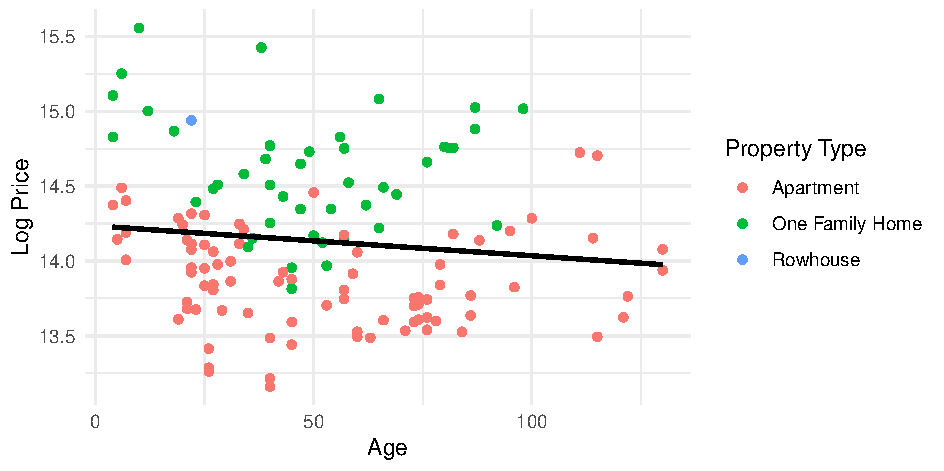
\includegraphics[width = 0.9\textwidth]{figures/Ordinary_Least_Squares/example_linear_regression.pdf}
    \caption{Age and log price of property sold in 2012 by Home in Aalborg.}
    \label{fig:example_simple_linear_regression}
\end{figure}

The dataset has observations $\{a_i, log(p_i)\}$ with $i = 1, \ldots, 130$. 
The age of the property is seen as the independent variable and the log price as the dependent variable.
We can assume, albeit naive considering figure \ref{fig:example_simple_linear_regression}, that there is a linear relationship between age and log price of the property in question.
This can be formulated as
\begin{align}\label{eq:approx_linear_relationship}
    \log(p) \approx b_0 + b_1 a
\end{align}
where $log(p)$ and $a$ denotes the log price and age respectively.
The right side \eqref{eq:approx_linear_relationship} is the model function in our case.
The function is on the form $f(a, \textbf{b})$, where $\textbf{b}$ is a $2 \times 1$ vector containing the coefficients $b_0$ and $b_1$.
The goal is now to find $\textbf{b}$ that minimizes the sum of squared residuals.
For the $i$'th observation the residual is defined as $r_i = log(p_i) - f(a_i, \textbf{b})$.
With the notation in place we can now write the sum of squared residuals as
\begin{align}
  \ssr(\textbf{b}) = \sum_{i = 1}^{130} r_i^2 &= \sum_{i = 1}^{130} \left( log(p_i) - f(a_i, \textbf{b}) \right)^2 \nonumber\\
  &= \sum_{i = 1}^{130} \left( log(p_i) - (b_0 + b_1 a_i) \right)^2.\label{eq:SSR}
\end{align}
The line that best fit the data is given by the $\textbf{b}$ that minimizes \eqref{eq:SSR} over all possible values $\textbf{b}$.
In the next section this optimization problem will be formulated with matrix notation.
The intuition provided here, using simple linear regression, can then be used in the case of multiple linear regression.
In the mean time the regression of log price on property age performed by \textbf{R} is shown in the table below.
\begin{table}[H]
    \centering
    \begin{tabular}{lrrrr}
        \toprule
        \textbf{term} & \textbf{estimate} & \textbf{std.error} & \textbf{statistic} & \textbf{p.value}\\
        \midrule
        Intercept & 14.2340997 & 0.0850712 & 167.319930 & 0.0000000\\
        Age & -0.0019912 & 0.0014324 & -1.390053 & 0.1669255\\
        \bottomrule
    \end{tabular}
    \caption{Regression coefficients from log price on age.}
    \label{tab:regress_log_price_on_age}
\end{table}
In table \ref{tab:regress_log_price_on_age} intercept refers to $b_0$ and age coefficient refers to $b_1$.
As $b_1$ is negative the data indicates a slight negative relationship between log price and age.
But as the p value is above 0.05 the relationship is regarded as statistically insignificant on a 95\% confidence level.
To fully grasp this concept, the concept of hypothesis testing will be introduced in chapter \ref{ch:hypothesis_testing}.

\subsection{Parameter Estimation in Matrix Form}
Estimating parameters for a multiple linear regression model in matrix form still translates to minimizing the sum of squared residuals, but the model function for the $i$'th observation can now be rewritten as
\begin{align*}
    \beta_0 + x_{i1} \beta_1 + \cdots + x_{ik}\beta_k =
    \begin{bmatrix} 
    1 & x_{i1} & \cdots & x_{ik}  
    \end{bmatrix} 
    \begin{bmatrix}
    \beta_0 \\ \beta_1 \\ \vdots \\ \beta_k
    \end{bmatrix} = \mathbf{x}_i \boldsymbol{\beta}.
\end{align*}
Where $\mathbf{x}_i$ denotes the $i$'th row in the design matrix $\mathbf{X}$.
Thus the sum of squared residuals is given by
\begin{align*}
    \ssr(\boldsymbol{\beta}) = \nsum (y_i - \mathbf{x}_i\boldsymbol{\beta})^2.
\end{align*}
% where $y_i$ denotes the price of property $i$ and $\mathbf{x}_i$ denotes the $i$'th row in the design matrix $\mathbf{X}$.
Suppose that $\betahat$ minimizes the sum of squared residuals, that is
\begin{align*}
    \betahat = \underset{\boldsymbol{\beta}}{\argmin} \nsum (y_i - \mathbf{x}_i\boldsymbol{\beta})^2.
\end{align*}
Where arg is the argument that minimizes the SSR w.r.t.$\!$ $\boldsymbol{\beta}$. Then $\betahat$ must satisfy the condition $\nabla \ssr(\betahat) = 0$.
Taking the derivative w.r.t. $\boldsymbol{\beta}$ yields
\begin{align}\label{eq:ssr_derivative}
    \frac{\partial \ssr(\boldsymbol{\beta})}{\partial \boldsymbol{\beta}} 
    =  \nsum -2(y_i - \mathbf{x}_i \boldsymbol{\beta})\mathbf{x}_i.
\end{align}
The expression $\nabla \ssr (\betahat) = 0$ can now be rewritten as
\begin{align*}
    \nsum -2(y_i - \mathbf{x}_i \betahat)\mathbf{x}_i = \mathbf{0} 
    \quad \Rightarrow \quad
    \nsum \mathbf{x}_i^\top(y_i - \mathbf{x}_i \betahat) = \mathbf{0}
\end{align*}
by taking the transpose and dividing by $-2$.
The condition is now a vector of size $(k + 1) \times 1$ and thus represents a system of $k + 1$ equations with $k + 1$ unknowns.
Writing the vector as a system of equations gives the following $k + 1$ equations
\begin{align}\label{eq:multiple_linear_regression_equations}
\begin{split}
    \nsum (y_i - \betahat_0 -  \mathbf{x}_{i1} \betahat_1 - \cdots - \betahat_k \mathbf{x}_{ik}) &= 0 \\
    \nsum \mathbf{x}_{i1}(y_i - \betahat_0 -  \mathbf{x}_{i1} \betahat_1 - \cdots - \betahat_k \mathbf{x}_{ik}) &= 0 \\
    &\vdots \\
    \nsum \mathbf{x}_{ik}(y_i - \betahat_0 -  \mathbf{x}_{i1} \betahat_1 - \cdots - \betahat_k \mathbf{x}_{ik}) &= 0.
\end{split}
\end{align}
Returning to the notation used in \eqref{eq:multiple_linear_regression_model}, \eqref{eq:multiple_linear_regression_equations} will now be rewritten to matrix notation
\begin{align} \label{eq:equation_to}
    \mathbf{X}^\top(\mathbf{y} - \mathbf{X}\betahat) &= \mathbf{0} \nonumber\\
    \mathbf{X}^\top\mathbf{y} - \mathbf{X}^\top\mathbf{X}\betahat &= \mathbf{0}\nonumber\\
    \mathbf{X}^\top\mathbf{X}\betahat &= \mathbf{X}^\top\mathbf{y}\label{eq:equation_from} \\
    \betahat &= \left(\mathbf{X}^\top\mathbf{X}\right)^{-1}\mathbf{X}^\top\mathbf{y}.
\end{align}
Going from \eqref{eq:equation_from} to \eqref{eq:equation_to} one must assume that $\mathbf{X}^\top\mathbf{X}$ is positive definite and thereby invertible.
It turns out that this is not the only assumption we have to make, there are in fact four assumptions related to the OLS estimator.
Together these assumptions are known as the Gauss-Markov assumptions. 
They will now be introduced.
\begin{assumption}[Linear in parameters]\label{as:linear_in_the_parameters}
    The model can be written as $\mathbf{y} = \mathbf{X}\boldsymbol{\beta} + \boldsymbol{\varepsilon}$ where $\mathbf{y}$ is an observed $n \times 1$ vector, $\mathbf{X}$ is an $n \times (k + 1)$ observed matrix, and $\boldsymbol{\varepsilon}$ is an $n \times 1$ vector of unobserved errors or disturbances \cite[p. 809]{Wooldridge2012}.
\end{assumption}
\begin{assumption}[No perfect collinearity]\label{as:no_perfect_collinearity}
    The matrix $\mathbf{X}$ has rank $(k + 1)$ \cite[p. 810]{Wooldridge2012}.
\end{assumption}
As the design matrix $\mathbf{X}$ has $n$ rows and $k + 1$ columns, assumption \ref{as:no_perfect_collinearity} implies that $n \geq k + 1$.
Moreover it implies that $\mathbf{X}$ has full column rank and thereby that $\mathbf{X}^\top\mathbf{X}$ is positive definite.
To prove this consider an arbitrary matrix $X$ of size $m \times n$.
The matrix $(X^\top X)$ is symmetric and positive semi definite, as for any $v \in \mathbb{R}^n$
\begin{align}\label{eq:positive_semi_definite}
v^\top (X^\top X) v = (v^\top X^\top) (X v) = (X v)^\top (X v) \geq 0.
\end{align}
Assume now that $X$ has rank $n$ and for contradiction that $v^\top X v = 0$.
By \eqref{eq:positive_semi_definite} this is a contradiction as it would imply that $vX = 0$ which cannot be true for a matrix of full column rank.
This is because a matrix of full column rank has columns that are linearly independent.
Thus it is proven that if $X$ has full column rank then $X^\top X$ is positive definite.
\begin{assumption}[Zero conditional mean]\label{as:zero_conditional_mean}
    Conditional on the entire matrix $\mathbf{X}$, each residual $\varepsilon_i$ has zero mean, i.e. \cite[p. 810]{Wooldridge2012}
    \begin{align*}
        E(\varepsilon_i | \mathbf{X}) = 0, \quad i = 1, 2, \ldots, n.
    \end{align*}
\end{assumption}
This assumption ensures that there is no correlation between each of the explanatory variables and $\varepsilon_i$ for $i = 1, \ldots, n$.
If it on the other hand was the case that $x_j$ were correlated with $\varepsilon_i$, the explanatory variable would be called an endogenous explanatory variable.
In the case that assumption \ref{as:zero_conditional_mean} holds and thereby that none of the explanatory variables are correlated with $\varepsilon_i$, we have what is called exogenous explanatory variables.
\begin{theorem}[Unbiasedness of OLS]\label{th:unbiasedness_of_ols}
    Under assumptions \ref{as:linear_in_the_parameters}, \ref{as:no_perfect_collinearity} and \ref{as:zero_conditional_mean}, the OLS estimator $\betahat$ is an unbiased estimator for $\boldsymbol{\beta}$ \cite[p. 810]{Wooldridge2012}.
\end{theorem}
\begin{proof}
    Under assumptions \ref{as:linear_in_the_parameters} and \ref{as:no_perfect_collinearity} we can write $\betahat$ as
    \begin{align}
        \betahat &= (\mathbf{X}^\top\mathbf{X})^{-1}\mathbf{X}^\top\mathbf{y} \nonumber\\
        &= (\mathbf{X}^\top\mathbf{X})^{-1}\mathbf{X}^\top(\mathbf{X}\boldsymbol{\beta} + \boldsymbol{\varepsilon}) \nonumber\\
        &=(\mathbf{X}^\top\mathbf{X})^{-1}\mathbf{X}^\top\mathbf{X}\boldsymbol{\beta} + (\mathbf{X}^\top\mathbf{X})^{-1}\mathbf{X}^\top\boldsymbol{\varepsilon} \nonumber\\
        &= \boldsymbol{\beta} + (\mathbf{X}^\top\mathbf{X})^{-1}\mathbf{X}^\top\boldsymbol{\varepsilon} \label{eq:beta_hat_unbiased}
    \end{align}
    Taking the conditional expectation of \eqref{eq:beta_hat_unbiased} on $\mathbf{X}$ and using the fact that $E(\boldsymbol{\varepsilon} | \mathbf{X}) = 0$ gives
    \begin{align*}
        E(\betahat | \mathbf{X}) &= \boldsymbol{\beta} + (\mathbf{X}^\top\mathbf{X})^{-1}\mathbf{X}^\top E(\boldsymbol{\varepsilon} | \mathbf{X}) \\
        &= \boldsymbol{\beta} + (\mathbf{X}^\top\mathbf{X})^{-1}\mathbf{X}^\top \mathbf{0} \\
        &= \boldsymbol{\beta}
    \end{align*}
    It is now shown that $\betahat$ is unbiased as defined in definition \ref{def:Unbiased_estmator} on page \pageref{def:Unbiased_estmator}.
\end{proof}

\subsection{Homoscedasticity and Heteroskedasticity}

In order to state the next assumption, we need a definition that enables us to describe the behaviour of the error terms.
The notion of homoscedasticity and heteroscedasticity will therefore be introduced here.

% In this section we wish to introduce \homo and \hetero. The section is based on \cite{Wooldridge2012}. First we define what \homo and \hetero is. 

\begin{definition}[Homoskedasticity and heteroskedasticity]
When the variance of the error term does not depend on the explanatory variables $\mathbf{X}$ and is constant, the errors is said to be homoscedastic, thus the errors should satisfy
\begin{align*}
    \var(\varepsilon | \mathbf{X}) = \var(\varepsilon) = \sigma^2.
\end{align*}
If this is not satisfied the error is said to be heteroskedastic. 
\end{definition}
The intuition behind homoscedasticity is that the variance of the error does not depend on the explanatory variables $\mathbf{X}$, hence it does not change for any value given to the explanatory variables. Conversely if the variance of the error term changes with any of the explanatory variables the error term is heteroskedastic. 

Homoskedasticity and heteroskedasticity can be illustrated as in figure \ref{fig:homo_with_dependent_up_axis} and \ref{fig:hetero_with_dependent_up_axis}. 
\begin{figure}[H]
\centering
\begin{subfigure}[b]{0.5\textwidth}
    \centering
    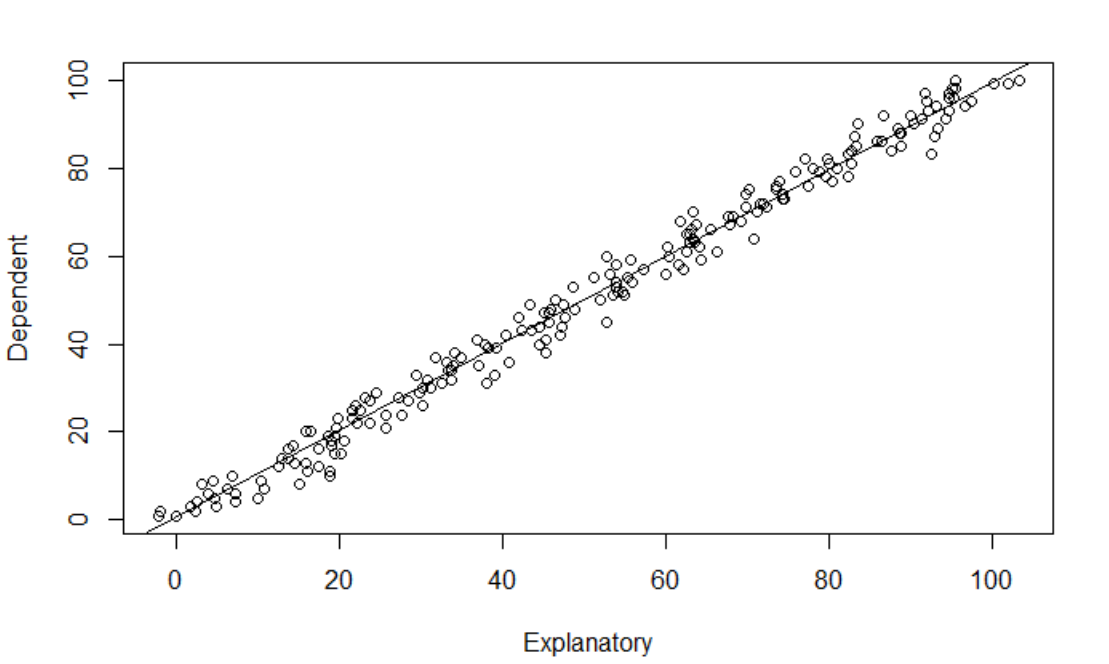
\includegraphics[width = \textwidth]{figures/Thea/homoplot.png}
    \caption{Homoskedasticity}
    \label{fig:homo_with_dependent_up_axis}
\end{subfigure}%
\begin{subfigure}[b]{0.5\textwidth}
\centering
    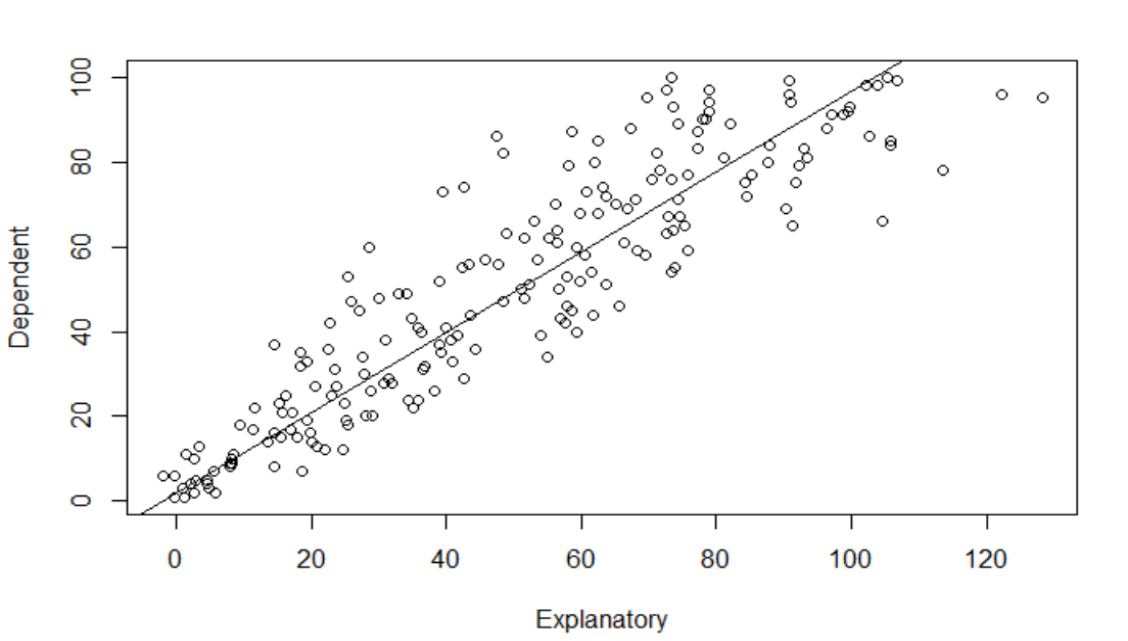
\includegraphics[width = \textwidth]{figures/Thea/Heteroplot.png}
    \caption{Heteroskedasticity}
    \label{fig:hetero_with_dependent_up_axis}
\end{subfigure}
\end{figure}
In the case of \homo  the variance is consistent for all values of $\mathbf{X}$, so the errors do not depend on the explanatory variables.
In the case of \hetero the variance changes as $\mathbf{X}$ changes. Typically the variance becomes greater as $\mathbf{X}$ becomes greater.

For an example you can consider a households income and its spending on luxury items. If the income is low most will be spend on necessity items such as food. If the income is high there is the possibility but not the guarantee of spending more on luxury items, thus there will be a greater variance in the consumption of luxury goods in the segment with higher household income. Heteroskedasticity can arise when variances of unobserved factors changes over different segments in the sample space. 

It is desired to have \homo rather than \hetero because \hetero will cause problems in statistical tests and linear regression, which will be investigated further in the section \ref{sec:consequence_of_hetero}. 

\subsection{OLS as the Best Linear Unbiased Estimator}
Now that the ideas of homoscedasticity and heteroscedasticity have been introduced, the next Gauss-Markov assumption can be stated.
\begin{assumption}[Homoskedasticity and no serial correlation]\label{as:homoskedasticity_and_no_serial_correlation}
    This assumption has two parts, the first part, regarding homoskedasticity states that
    \begin{align*}
       \var(\varepsilon_i | \mathbf{X}) = \sigma^2, \quad i = 1,2, \ldots, n.
    \end{align*}
    The second part, regarding serial correlation, states that
    \begin{align*}
        \cov(\varepsilon_i, \varepsilon_j | \mathbf{X}) = 0, \quad \text{for all} \ i \neq j.
    \end{align*}
    In matrix form these two assumptions together become
    \begin{align*}
        \var(\boldsymbol{\varepsilon} | \mathbf{X}) = \sigma^2\mathbf{I}_{n\times n}.
    \end{align*}
\end{assumption}

With the previous assumption in place, we are now able to derive the variance-covariance matrix of the OLS estimator.
\begin{theorem}[Variance-Covariance Matrix of the OLS Estimator]\label{th:variance-covariance_of_the_ols_estimator}
    Under assumptions \ref{as:linear_in_the_parameters}, \ref{as:no_perfect_collinearity}, \ref{as:zero_conditional_mean} and \ref{as:homoskedasticity_and_no_serial_correlation} the conditional variance of $\betahat$ on $\mathbf{X}$ satisfies \cite[p. 811]{Wooldridge2012} 
    \begin{align*}
        \var(\betahat | \mathbf{X}) = \sigma^2(\mathbf{X}^\top\mathbf{X})^{-1}.
    \end{align*}
\end{theorem}
\begin{proof}
    From \eqref{eq:beta_hat_unbiased} we have
    \begin{align}
        \var(\betahat | \mathbf{X}) &= \var\left[ (\mathbf{X}^\top\mathbf{X})^{-1}\mathbf{X}^\top\boldsymbol{\varepsilon}|\mathbf{X} \right] \nonumber\\
        &= (\mathbf{X}^\top\mathbf{X})^{-1}\mathbf{X}^\top\left[ \var(\boldsymbol{\varepsilon} | \mathbf{X}) \right] \mathbf{X}(\mathbf{X}^\top\mathbf{X})^{-1}, \label{eq:conditional_variance_of_epsilon}
    \end{align}
    and we can now use assumption \ref{as:homoskedasticity_and_no_serial_correlation} to substitute $\var(\boldsymbol{\varepsilon}|\mathbf{X})$ for $\left[\sigma^2 \mathbf{I}\right]$ in \eqref{eq:conditional_variance_of_epsilon} which gives
    \begin{align*}
        \var(\betahat | \mathbf{X}) &= (\mathbf{X}^\top\mathbf{X})^{-1}\mathbf{X}^\top\left[\sigma^2 \mathbf{I}\right] \mathbf{X}(\mathbf{X}^\top\mathbf{X})^{-1} \\
        &= \sigma^2(\mathbf{X}^\top\mathbf{X})^{-1}\mathbf{X}^\top \mathbf{X}(\mathbf{X}^\top\mathbf{X})^{-1} \\
        &= \sigma^2(\mathbf{X}^\top\mathbf{X})^{-1}
    \end{align*}
\end{proof}

As it was explained in conjunction with defintion \ref{def:minimum_mean_square_error}, on page \pageref{def:minimum_mean_square_error}, the BLUE is the estimator that has the smallest variance.
It is possible to establish conditions that any linear unbiased estimator must satisfy, these conditions can then be used to find an expression for the variance of any linear unbiased estimator.
Thus we can compare the variance of the OLS estimator and of any linear unbiased estimator.
This is the motivation for the following theorem, better known as the Gauss-Markov theorem.
\begin{theorem}[Gauss-Markov Theorem]
    Under assumptions \ref{as:linear_in_the_parameters}, \ref{as:no_perfect_collinearity}, \ref{as:zero_conditional_mean} and \ref{as:homoskedasticity_and_no_serial_correlation} 
    \begin{align}\label{eq:betahat_y}
        \betahat &= (\mathbf{X}^\top\mathbf{X})^{-1}\mathbf{X}^\top\mathbf{y}
    \end{align}
    is the best linear unbiased estimator \cite[p. 811]{Wooldridge2012}.
\end{theorem}\label{th:gauss_markoc_theorem}
\begin{proof}
    Any linear estimator $\betahat$ can be written as
    \begin{align}\label{eq:any_linear_operator}
        \boldsymbol{\Tilde{\beta}} = \mathbf{A}^\top \mathbf{y},
    \end{align}
    where $\mathbf{A}$ is an $n \times (k + 1)$ matrix.
    For the linear estimator to be unbiased conditional on $\mathbf{X}$ it must satisfy
    \begin{align}\label{eq:condition_of_unbiasedness}
        E(\betatilde|\mathbf{X}) = \boldsymbol{\beta}.
    \end{align}
    Following that $\mathbf{y} = \mathbf{X}\boldsymbol{\beta} + \boldsymbol{\varepsilon}$ the expectation of $\betatilde$ conditional on $\mathbf{X}$ can be written as
    \begin{align}
       E(\betatilde|\mathbf{X}) &= E( \mathbf{A}^\top\mathbf{X}\boldsymbol{\beta} + \mathbf{A}^\top\boldsymbol{\varepsilon}|\mathbf{X} )\nonumber \\
        &=  \mathbf{A}^\top\mathbf{X}\boldsymbol{\beta} + E( \mathbf{A}^\top\boldsymbol{\varepsilon}|\mathbf{X} )\nonumber \\
        &=\mathbf{A}^\top\mathbf{X}\boldsymbol{\beta} +  \mathbf{A}^\top E( \boldsymbol{\varepsilon}|\mathbf{X} )\nonumber \\
        &=\mathbf{A}^\top\mathbf{X}\boldsymbol{\beta}\label{eq:expectation_of_any_linear_unbiased_estimator}
    \end{align}
    For the linear estimator to be unbiased it must be that \eqref{eq:expectation_of_any_linear_unbiased_estimator} is equal to the left side of \eqref{eq:condition_of_unbiasedness}, as below
    \begin{align}\label{eq:unbiasedness_identity}
        \mathbf{A}^\top\mathbf{X}\boldsymbol{\beta} = \boldsymbol{\beta}
    \end{align}
    The relation in \eqref{eq:unbiasedness_identity} holds if and only if $\mathbf{A}^\top\mathbf{X} = \mathbf{I}_{k + 1}$, which furthermore implies that $(\mathbf{A}^\top\mathbf{X})^\top = \mathbf{X}^\top\mathbf{A} = \mathbf{I}_{k + 1}$.
    The variance of $\betatilde$ conditional on $\mathbf{X}$ is given by
    \begin{align}
        \var(\betatilde|\mathbf{X}) &= \var(\mathbf{A}^\top\mathbf{X}\boldsymbol{\beta} + \mathbf{A}^\top\boldsymbol{\varepsilon}|\mathbf{X}) \nonumber\\
        &= \var(\mathbf{A}^\top\mathbf{X}\boldsymbol{\beta}|\mathbf{X}) + \var(\mathbf{A}^\top\boldsymbol{\varepsilon}|\mathbf{X}) + 2 \cov\left(\mathbf{A}^\top\mathbf{X}\boldsymbol{\beta},\mathbf{A}^\top\boldsymbol{\varepsilon}|\mathbf{X}\right) \nonumber\\
        &= \var(\mathbf{A}^\top\boldsymbol{\varepsilon}|\mathbf{X}) \nonumber\\
        &= \mathbf{A}^\top\var(\boldsymbol{\varepsilon}|\mathbf{X})\mathbf{A}.\label{eq:variance_of_betatilde_conditional_on_x}
    \end{align}
    From assumption \ref{as:homoskedasticity_and_no_serial_correlation} and \eqref{eq:variance_of_betatilde_conditional_on_x} we conclude that
    \begin{align}
        \var(\betatilde|\mathbf{X}) = \sigma^2\mathbf{A}^\top\mathbf{A}
    \end{align}
    Knowing the variance of any linear unbiased estimator we can now subtract the known variance of the OLS estimator, which was found in theorem \ref{th:variance-covariance_of_the_ols_estimator}
    \begin{align}
        \var(\betatilde|\mathbf{X}) - \var(\betahat|\mathbf{X}) &= \sigma^2\mathbf{A}^\top\mathbf{A} - \sigma^2(\mathbf{X}^\top\mathbf{X})^{-1} \nonumber \\
        &= \sigma^2\left[\mathbf{A}^\top\mathbf{A} - (\mathbf{X}^\top\mathbf{X})^{-1} \right] \label{eq:subtraction_of_variances1} \\
        &= \sigma^2\left[\mathbf{A}^\top\mathbf{A} - \mathbf{A}^\top\mathbf{X}(\mathbf{X}^\top\mathbf{X})^{-1}\mathbf{X}^\top\mathbf{A} \right] \label{eq:subtraction_of_variances2} \\
        &= \sigma^2\mathbf{A}^\top\left[\mathbf{I} - \mathbf{X}(\mathbf{X}^\top\mathbf{X})^{-1}\mathbf{X}^\top \right]\mathbf{A}.\label{eq:subtraction_of_variances3}
    \end{align}
    Going from \eqref{eq:subtraction_of_variances1} to \eqref{eq:subtraction_of_variances2} we use the fact that $\mathbf{A}^\top\mathbf{X} = \mathbf{X}^\top\mathbf{A} = \mathbf{I}_{k+1}$.
    Let 
    \begin{align}\label{eq:projection_matrix}
    \mathbf{H} = \mathbf{X}(\mathbf{X}^\top\mathbf{X})^{-1}\mathbf{X}^\top,
    \end{align}
    and notice that
    \begin{align*}
        \left(\mathbf{I} - \mathbf{H}\right)^\top &= (\mathbf{I} - \mathbf{X}(\mathbf{X}^\top\mathbf{X})^{-1}\mathbf{X}^\top)^\top 
        = (\mathbf{I})^\top - \left(\mathbf{X}^\top\right)^\top\left[(\mathbf{X}^\top\mathbf{X})^{-1}\right]^\top\mathbf{X}^\top \\
        &= \mathbf{I} - \left(\mathbf{X}^\top\right)^\top\left[(\mathbf{X}^\top\mathbf{X})^{-1}\right]^\top\mathbf{X}^\top
        = \mathbf{I} - \mathbf{X}\left[(\mathbf{X}^\top\mathbf{X})^\top\right]^{-1}\mathbf{X}^\top \\
        &= \mathbf{I} - \mathbf{X}\left[\mathbf{X}^\top\left(\mathbf{X}^\top\right)^\top\right]^{-1}\mathbf{X}^\top 
        = \mathbf{I} - \mathbf{X}\left(\mathbf{X}^\top\mathbf{X}\right)^{-1}\mathbf{X}^\top = \left(\mathbf{I} - \mathbf{H}\right),
    \end{align*}
    showing that $\mathbf{H}$ is symmetric.
    Notice also that
    \begin{align*}
        \left(\mathbf{I} - \mathbf{H}\right)^2 &= \left(\mathbf{I} - \mathbf{H}\right)^\top\left(\mathbf{I} - \mathbf{H}\right) = (\mathbf{I} - \mathbf{X}\left(\mathbf{X}^\top\mathbf{X}\right)^{-1}\mathbf{X}^\top)(\mathbf{I} - \mathbf{X}\left(\mathbf{X}^\top\mathbf{X}\right)^{-1}\mathbf{X}^\top) \\
        &= \mathbf{I} - 2\mathbf{X}\left(\mathbf{X}^\top\mathbf{X}\right)^{-1}\mathbf{X}^\top + \mathbf{X}\left(\mathbf{X}^\top\mathbf{X}\right)^{-1}\mathbf{X}^\top\mathbf{X}\left(\mathbf{X}^\top\mathbf{X}\right)^{-1}\mathbf{X}^\top \\
        &= \mathbf{I} - 2\mathbf{X}\left(\mathbf{X}^\top\mathbf{X}\right)^{-1}\mathbf{X}^\top + \mathbf{X}\left(\mathbf{X}^\top\mathbf{X}\right)^{-1}\mathbf{X}^\top = \left(\mathbf{I} - \mathbf{H}\right)
    \end{align*}
    showing that $\left(\mathbf{I} - \mathbf{H}\right)$ is idempotent.
    As $\left(\mathbf{I} - \mathbf{H}\right)$ is both symmetric and idempotent it is called a projection matrix.
    Using $\left(\mathbf{I} - \mathbf{H}\right)$ and \eqref{eq:subtraction_of_variances3} we can write
    \begin{align}\label{eq:positive_semi_definite_subtraction}
        \var(\betatilde|\mathbf{X}) - \var(\betahat|\mathbf{X}) &= \sigma^2\mathbf{A}^\top\left(\mathbf{I} - \mathbf{H}\right)\mathbf{A}.
    \end{align}
    As $\left(\mathbf{I} - \mathbf{H}\right)$ is a projection matrix we can now show that \eqref{eq:positive_semi_definite_subtraction} is positive semi definite using first idempotence and then symmetry
    \begin{align*}
        \sigma^2\mathbf{A}^\top\left(\mathbf{I} - \mathbf{H}\right)\mathbf{A} &= \sigma^2\mathbf{A}^\top\left(\mathbf{I} - \mathbf{H}\right)^2\mathbf{A} = \sigma^2\mathbf{A}^\top\left(\mathbf{I} - \mathbf{H}\right)^\top\left(\mathbf{I} - \mathbf{H}\right)\mathbf{A}\\
        &= \sigma^2\left[\left(\mathbf{I} - \mathbf{H}\right)\mathbf{A}\right]^\top\left(\mathbf{I} - \mathbf{H}\right)\mathbf{A} \geq 0.
    \end{align*}
    It has now been shown that the variance of any linear unbiased operator is greater than or equal to the variance of the OLS estimator, or in other words the OLS estimator is the BLUE.
\end{proof}

% \subsection{Consequences of Heteroscedasticity}
% In this sections we wish to determine how \hetero will affect both OLS, \textit{t-statistics}, \textit{F-statistics} and \textit{confidence intervals}. 

% First we wish to determine if the estimator $\betahat$ is unbiased or biased in the presence of heteroskedasticity.  

% Remember assumption \ref{as:linear_in_the_parameters}, \ref{as:no_perfect_collinearity} and \ref{as:zero_conditional_mean}. If these hold theorem \ref{th:unbiasedness_of_ols} proved that the OLS estimator $\betahat$ is unbiased for $\boldsymbol{\beta}$, which is the same as $E[\hat{\beta}_j] = \beta_j
% $ for $j = 1,2, \ldots, k$. 

% Because the error terms in $\var(\boldsymbol{\varepsilon} | \mathbf{X})$ did no determine whether the OLS was biased or unbiased in the theorem and its proof, the presence of \hetero will not cause $\betahat$ to be biased. 

% Next we wish to determine how our measure-of-fit test $\mathcal{R}^2$ is influenced by \hetero. 
% $\mathcal{R}^2$ measures how much of the variance in the dependent variable is explained by the independent variables. In our model it determines how much of the variance in $y$ is explained in the variables $\mathbf{X}$. 
% Low values of $\mathcal{R}^2$ makes predictions difficult because most of the variance in $y$ is caused by unobserved factors in $\varepsilon$, so the OLS predictions will be hard to calculate given a set of explanatory variables.
% Consider the expression for $\mathcal{R}^2$
% \begin{align*}
%     \mathcal{R}^2 = 1 - \dfrac{SSR}{SST}
% \end{align*}
% Where \textbf{SSR} is the \textbf{sum of squared residuals} given as
% \begin{align*}
%     SSR \equiv \nsum \hat{\varepsilon}_i^2
% \end{align*}
% and \textbf{SST} is the \textbf{total sum of squares} given as
% \begin{align*}
%     SST \equiv \nsum (y_i - \overline{y})^2. 
% \end{align*}
% The $\mathcal{R}^2$ value is between $0$ and $1$. The closer the value is to one $1$ the more of the variance is accounted for in the explanatory variables, thus it is desireable to have an $\mathcal{R}^2$ value close to $1$.
% This coefficient of determination can be changed to the adjusted $\mathcal{R}^2$ as
% \begin{align*}
%     \mathcal{R}^2_{Adj} = 1 - \dfrac{SSR/(n - k - 1)}{SST/(n - 1)}
% \end{align*}
% This rewriting of the model adjusts for the number of predictors in the model. This $\mathcal{R}^2$ in- and decreases if a predictor improves more or less than expected, respectively. 

% Both SSR and SST are unconditional variances in $\mathcal{R}^2$, thus they are not influenced by the presence of \hetero.  

% This means that \hetero does not cause the OLS estimators to be biased or inconsistent and nor does it affect the $\mathcal{R}^2$ test, however it will cause the variance of the OLS estimators, i.e. $\var(\betahat)$, to be biased, which will be explained next.  

% The \homo assumption is $\var(\boldsymbol{\varepsilon} | \mathbf{X}) = \sigma^2$. If assumption \ref{as:linear_in_the_parameters}, \ref{as:no_perfect_collinearity}, \ref{as:zero_conditional_mean} and \ref{as:homoskedasticity_and_no_serial_correlation} hold the variance of the OLS estimator can be expressed as in theorem \ref{th:variance-covariance_of_the_ols_estimator}, which implies that variance of $\betahat$ given the explanatory variables has an explicit form given as
% \begin{align*}
%     \var(\betahat | \mathbf{X}) = \sigma^2(\mathbf{X}^\top\mathbf{X})^{-1}.
% \end{align*}
% The slope coefficients can be defined as 
% \begin{align}\label{eq:slope_variance_OLS_estimator}
%     \var(\hat{\beta}_j|\mathbf{X}) = \dfrac{\sigma^2}{SST_j(1- \mathcal{R}_j^2)}
% \end{align}
% Where $j = 1, \ldots, k$ and $SST_j = \nsum (x_{ij} - \overline{x}_j)^2$ is the total sample variation in $x_j$ and $\mathcal{R}^2_j$ is found from a regression on $x_j$ with all other independent variables. 

% Equation \eqref{eq:slope_variance_OLS_estimator} depends on $\sigma^2$, $SST_j$ and $\mathcal{R}^2_j$.
% Here $\sigma^2$ is an unknown variable, the larger $\sigma^2$ the larger are the variances for the OLS estimators. $SST_j$ is the total sample variation in $x_j$, the larger it is the smaller will the variance of the OLS estimators be so it is preferred to have as much sample variation as possible which can be obtained by increasing sample size. 
% Notice that $\mathcal{R}^2_j$ is found with a regression involving only the independent variables in the original model, where $x_j$ is the dependent variable. This differs from the $\mathcal{R}^2$ found by regression on $y$ with $x_1, \ldots, x_k$ as the independent variables. 
% Consider the example $y = \betahat_0 + \betahat_1 x_1 + \betahat_2 x_2 + \varepsilon$, here $\mathcal{R}^2_1$ is found by making a regression of $x_1$ on $x_2$. 
% As always an $\mathcal{R}^2_1$ value close to one means that $x_2$ explains much of the variation in $x_1$, so a value close to $1$ means that $x_1$ and $x_2$ are highly correlated.
% $\mathcal{R}^2_j$ tests how much of the variation in one of the independent variables is explained from the remaining independent variables.
% The best estimator for $\betahat_j$ is found with a low value of $\mathcal{R}^2_j$, thus a smaller relationship between the explanatory variables is desired when retrieving $\var(\betahat_j)$. Note $\mathcal{R}^2$ cannot equal $0$ due to assumption \ref{as:no_perfect_collinearity}. 

% From \eqref{eq:slope_variance_OLS_estimator} it is possible to find the standard deviation of $\betahat_j$, which is the squre root of \ref{eq:slope_variance_OLS_estimator}, which is
% \begin{align}\label{eq:standard_deviation}
%     sd(\betahat_j) = \dfrac{\sigma}{SST_j(\big(1- \mathcal{R}_j^2)\big)^{1/2}}
% \end{align}
% The standard deviation, $\sigma$, is replaced by its estimate to obtain the standard error
% \begin{align}\label{eq:standad_error}
%     se(\betahat_j) = \dfrac{\hat{\sigma}}{SST_j(\big(1- \mathcal{R}_j^2)\big)^{1/2}}
% \end{align}
% Note that the standard deviation measures the dispersion a data set has from the mean, whereas the standard errors measures how far the sample mean of the data is likely to be from the true sample space mean. 

% Since \eqref{eq:standad_error} is obtained from \eqref{eq:slope_variance_OLS_estimator}, which relies on \homo the standard error will not be a valid estimator of the standard deviation in \eqref{eq:standard_deviation} in the presence of \hetero. This means that \hetero will cause bias in the $\var(\betahat_j)$ which invalidates the standard errors, $\varepsilon$. 

% Furthermore \textit{confidence intervals}, \textit{t-statistics} and \textit{F-statistics} will no longer follow a normal distribution and thus their results will be invalid when \hetero is present. 

% The OLS is the \textbf{best linear unbiased estimator (BLUE)}, if assumption  \ref{as:linear_in_the_parameters}, \ref{as:no_perfect_collinearity}, \ref{as:zero_conditional_mean} and \ref{as:homoskedasticity_and_no_serial_correlation} holds.
% In the Gauss-Markov theorem \ref{th:gauss_markoc_theorem}, it is seen that in order for the OLS to be the BLUE it is a necessary for the \homo assumption to hold true, otherwise it would not have the smallest variance of the estimators causing it to not be the best estimator.

% In addition it is possible to determine an unbiased estimator $\sigma^2$. 
% In order for $\sigma^2$ to be unbiased it must satisfy $E[\varepsilon^2] = \sigma^2$.  This is the same as $\sigma^2 = \dfrac{1}{n}\nsum \varepsilon_i^2$.
% This is not an estimator because we do not observe $\varepsilon$. Instead isolate the error term in the OLS as $\varepsilon_i = y_i - \beta_0 - \beta_1x_{i1} - \ldots - \beta_kx_{ik}$, where $\mathbf{\beta}_j$ is unknown. 
% In order to get OLS error term we must know $\mathbf{\beta}_j$, so we replace it with its estimate so
% \begin{align*}
%      \hat{\varepsilon}_i = y_i - \hat{\beta_0} - \hat{\beta_1x_{i1}} - \ldots - \hat{\beta}_kx_{ik}.
% \end{align*}
% We can now estimate $\sigma^2$ as
% \begin{align}\label{eq:OLS_estimate_sigma_i_anden}
%     \hat{\sigma}^2 &= \dfrac{\nsum \hat{\varepsilon}^2_i}{n-k-1}\nonumber \\
%     &= \dfrac{SSR}{n-k-1}
% \end{align}
% Where $n-k-1$ is the degrees of freedom in the OLS with $n$ observations and $k$ independent variables. 
% Note $n-k-1$ is the number of observations subtracted the number of estimated parameters. 
% To derive the variance-covariance matrix for the OLS estimator we need to make an assumption regarding the variance of the error term. 
% This assumption involves homoskedasticity, so to fully understand the concept it will be introduced in the following section.
% \vspace{5mm}
% \hrule
% \vspace{5mm}
\subsection{Estimating the variance of the error term}
Next we are interested in quantifying the term $\sigma^2$, as $\var(\betahat|\mathbf{X})$ depends on this constant.
As previously stated $\sigma^2$ is the variance of the error term
\begin{align*}
    \sigma^2 = \var(\varepsilon_i) =  E\left[\Big(\varepsilon_i - E(\varepsilon_i)\Big)^2\right] = E\left[\varepsilon_i^2\right],
\end{align*}
the last equality holds as $E(\varepsilon_i) = 0$.
The MLE for $\sigma^2$ is given by \eqref{eq:MLE_for_sigma} and repeated below
\begin{align}\label{eq:MLE_for_sigma_omskrevet}
    \hat{\sigma}^2 &= \frac{\|\textbf{y} - \textbf{X}( \textbf{X}^\top\textbf{X} )^{-1}\textbf{X}^\top\textbf{y}\|^2}{n}
    = \dfrac{1}{n}\sum_{i=1}^n \left(y_i - \mathbf{x}_i\betahat\right)^2.
\end{align}
% it was found in chapter \ref{ch:likelihood_theory} on page \pageref{eq:MLE_for_sigma
If we by $\hat{\varepsilon}_i$ denote the $i$'th residual, then
\begin{align}\label{eq:observed_residual}
    \hat{\varepsilon}_i = y_i - \mathbf{x}_i\betahat.
\end{align}
Inserting \eqref{eq:observed_residual} into \eqref{eq:MLE_for_sigma_omskrevet} the MLE becomes
\begin{align}\label{eq:valid_estimate}
    \hat{\sigma}^2 = \dfrac{1}{n}\sum_{i=1}^n \hat{\varepsilon}_i^2.
\end{align}
The sum in \eqref{eq:valid_estimate} is equal to $\ssr(\betahat)$ yielding a third expression for the MLE
\begin{align}
    \hat{\sigma}^2 = \frac{\ssr(\betahat)}{n}.
\end{align}
Regardless of the chosen expression, the MLE is a biased estimate.
% \vspace{1ex}
% \hrule
% \vspace{1ex}
% If the values of $\varepsilon_i^2$ a way to estimate the expectation of a $\varepsilon_i^2$ is to use the sample average, which in this case would be
% \begin{align}\label{eq:sample_average}
%     \dfrac{1}{n}\nsum \varepsilon_i^2.
% \end{align}
% However \eqref{eq:sample_average} is not a feasible estimator as $\varepsilon_i = y_i - \mathbf{x}_i\boldsymbol{\beta}$ is unknown to us because we do not have the true $\boldsymbol{\beta}$.
% We do however have an estimate $\betahat$ we can use to obtain an estimate for $\varepsilon_i$, lets denote the estimate
% \begin{align}\label{eq:observed_residual}
%     \hat{\varepsilon}_i = y_i - \mathbf{x}_i\betahat.
% \end{align}
% In other words this is the observed residual and it will be investigated further in section \ref{subsec:residuals}.
% We can now insert \eqref{eq:observed_residual} into \eqref{eq:sample_average} to obtain a feasible estimate for $\sigma^2$
% \begin{align}\label{eq:valid_estimate}
%     \dfrac{1}{n}\sum_{i=1}^n \hat{\varepsilon}_i^2 = \dfrac{1}{n}\sum_{i=1}^n \left(y_i - \mathbf{x}_i\betahat\right)^2 = \frac{\ssr(\betahat)}{n}.
% \end{align}
% Although the estimate \eqref{eq:valid_estimate} is valid, it turns out to be biased.
% \vspace{1ex}
% \hrule
% \vspace{1ex}
This is because the estimate does not take into account the first order conditions imposed on the residuals.
The first order conditions are the $k + 1$ equations in \eqref{eq:multiple_linear_regression_equations} on page \pageref{eq:multiple_linear_regression_equations}.
The intuition being that if we know $n - (k + 1)$ of the residuals the rest can be found using the first order conditions, which in this case becomes a system of $k + 1$ equations with $k + 1$ unknowns. 
Because of this there is only $n - (k + 1)$ degrees of freedom in the residuals compared to $n$ in the error terms \cite[p. 55]{Wooldridge2012}.
Taking this into account the unbiased estimator of $\sigma^2$ is now presented as
\begin{align} \label{eq:sigma_hat_2_n-k-1}
    \hat{\sigma}^2 = \frac{\ssr(\betahat)}{n - (k + 1)} = \frac{\ssr(\betahat)}{n - k - 1}.
\end{align}
To prove that this estimator is in fact unbiased, the following theorem is presented,
% \vspace{5mm}
% \hrule
% \vspace{5mm}
\begin{theorem}[Unbiasedness of $\sigmahat$]
    Under assumptions \ref{as:linear_in_the_parameters}, \ref{as:no_perfect_collinearity}, \ref{as:zero_conditional_mean} and \ref{as:homoskedasticity_and_no_serial_correlation}, the estimator $\hat{\sigma}^2$, in \eqref{eq:sigma_hat_2_n-k-1}, is unbiased for $\sigma^2:E(\hat{\sigma}^2|\mathbf{X}) = \sigma^2$ for all $\sigma^2 > 0$ \cite[p. 813]{Wooldridge2012}.
\end{theorem}
\begin{proof}
    Consider the relationship $\mathbf{y} = \mathbf{X}\betahat + \boldsymbol{\hat{\varepsilon}}$.
    We start by isolating $\boldsymbol{\hat{\varepsilon}}$
    \begin{align*}
        \boldsymbol{\hat{\varepsilon}} = \mathbf{y} - \mathbf{X}\betahat.
    \end{align*}
    Now $\betahat$ can be replaced by $\left(\mathbf{X}^\top\mathbf{X}\right)^{-1}\mathbf{X}^\top\mathbf{y}$, see \eqref{eq:equation_to} on page \pageref{eq:equation_to}, and \eqref{eq:projection_matrix} can be used to rewrite the expression 
    \begin{align}
        \hat{\boldsymbol{\varepsilon}} = \mathbf{y} - \mathbf{X}\left(\mathbf{X}^\top\mathbf{X}\right)^{-1}\mathbf{X}^\top\mathbf{y}
        = \left(\mathbf{I} - \mathbf{H}\right)\mathbf{y}. \label{eq:replace_with_y}
    \end{align}
    Using the relationship stated at the beginning of this proof lets us rewrite \eqref{eq:replace_with_y} as
    \begin{align*}
        \boldsymbol{\hat{\varepsilon}} &= \left(\mathbf{I} - \mathbf{H}\right)\left(\mathbf{X}\betahat + \boldsymbol{\hat{\varepsilon}}\right) 
        = \left(\mathbf{I} - \mathbf{H}\right)\mathbf{X}\betahat + \left(\mathbf{I} - \mathbf{H}\right)\boldsymbol{\hat{\varepsilon}}
        = \left(\mathbf{I} - \mathbf{H}\right)\mathbf{X}\betahat + \left(\mathbf{I} - \mathbf{H}\right)\boldsymbol{\varepsilon}\\
        &= \mathbf{X}\betahat - \mathbf{H}\mathbf{X}\betahat + \boldsymbol{\varepsilon} - \mathbf{H}\boldsymbol{\varepsilon}
        = \mathbf{X}\betahat - \mathbf{X}\left(\mathbf{X}^\top\mathbf{X}\right)^{-1}\mathbf{X}^\top\mathbf{X}\betahat + \boldsymbol{\varepsilon} - \mathbf{X}\left(\mathbf{X}^\top\mathbf{X}\right)^{-1}\mathbf{X}^\top\boldsymbol{\varepsilon} \\
        &= \mathbf{X}\betahat - \mathbf{X}\betahat + \boldsymbol{\varepsilon} - \mathbf{X}\left(\mathbf{X}^\top\mathbf{X}\right)^{-1}\mathbf{X}^\top\boldsymbol{\varepsilon} 
        = \boldsymbol{\varepsilon} - \mathbf{X}\left(\mathbf{X}^\top\mathbf{X}\right)^{-1}\mathbf{X}^\top\boldsymbol{\varepsilon} = \left(\mathbf{I} - \mathbf{H}\right)\boldsymbol{\varepsilon}.
    \end{align*}
    In the third equality we use $(\textbf{I} - \textbf{H})\hat{\boldsymbol{\varepsilon}} = (\textbf{I} - \textbf{H})^2\boldsymbol{\varepsilon} = (\textbf{I} - \textbf{H})\boldsymbol{\varepsilon}$.
    Because $\left(\mathbf{I} - \mathbf{H}\right)$ is a projection matrix then
    \begin{align*}
        \boldsymbol{\hat{\varepsilon}}^\top\boldsymbol{\hat{\varepsilon}} = \left[  \left(\mathbf{I} - \mathbf{H}\right)\boldsymbol{\varepsilon} \right]^\top\left[ \left(\mathbf{I} - \mathbf{H}\right)\boldsymbol{\varepsilon} \right] = \boldsymbol{\varepsilon}^\top\left(\mathbf{I} - \mathbf{H}\right)^\top \left(\mathbf{I} - \mathbf{H}\right)\boldsymbol{\varepsilon} = \boldsymbol{\varepsilon}^\top \left(\mathbf{I} - \mathbf{H}\right)\boldsymbol{\varepsilon}.
    \end{align*}
    Furthermore because $\boldsymbol{\varepsilon}^\top \left(\mathbf{I} - \mathbf{H}\right)\boldsymbol{\varepsilon}$ is a scalar, it is equal to its trace.
    Thus we can rewrite the expectation of $\boldsymbol{\varepsilon}^\top \left(\mathbf{I} - \mathbf{H}\right)\boldsymbol{\varepsilon}$ conditional on $\mathbf{X}$ using this fact
    % \begin{center}
    %     \titlerule
    %     \Large{\textbf{Her er nogle traceregler som jeg lige skal have kigget på, og måske skrive lidt mere ud.}}
    %     \titlerule
    % \end{center}
    \begin{align}
        E\left[\boldsymbol{\varepsilon}^\top \left(\mathbf{I} - \mathbf{H}\right)\boldsymbol{\varepsilon}|\mathbf{X}\right] &= E\left[\tr\left(\boldsymbol{\varepsilon}^\top \left(\mathbf{I} - \mathbf{H}\right)\boldsymbol{\varepsilon}\right)|\mathbf{X}\right] 
        = E\left[\tr\left(\left(\mathbf{I} - \mathbf{H}\right)\boldsymbol{\varepsilon}\boldsymbol{\varepsilon}^\top\right)|\mathbf{X}\right] \nonumber\\
        &= \tr\left[E\left(\left(\mathbf{I} - \mathbf{H}\right)\boldsymbol{\varepsilon}\boldsymbol{\varepsilon}^\top|\mathbf{X}\right)\right] 
        = \tr\left[\left(\mathbf{I} - \mathbf{H}\right)E\left(\boldsymbol{\varepsilon}\boldsymbol{\varepsilon}^\top|\mathbf{X}\right)\right] \nonumber\\
        &= \tr\left[\left(\mathbf{I} - \mathbf{H}\right)\sigma^2\mathbf{I}_{n}\right]
        = \sigma^2\tr\left[\left(\mathbf{I} - \mathbf{H}\right)\right]. \label{eq:trace_projection_matrix}
    \end{align}
    In the above computation we use the fact that the trace of a product are invariant under cyclical permutations of the factors and that the trace and expectation commutes as the trace is a linear operator. 
    Notice that the trace of $\left(\mathbf{I} - \mathbf{H}\right)$ can be rewritten as
    \begin{align*}
        \tr\left[\left(\mathbf{I}_n - \mathbf{H}\right)\right] &= \tr(\mathbf{I}_n) - \tr\left[\mathbf{X}(\mathbf{X}^\top\mathbf{X})^{-1}\mathbf{X}^\top\right] \\
        &= n - \tr\left[ (\mathbf{X}^\top\mathbf{X})^{-1}\mathbf{X}^\top\mathbf{X} \right] \\
         &= n - \tr\left[\mathbf{I}_{k + 1} \right] \\
        &= n - (k + 1) = n - k - 1.
    \end{align*}
    Therefore,
    \begin{align*}
        E\left(\hat{\sigma}^2|\mathbf{X}\right) &= \frac{E\left[\ssr(\betahat)|\textbf{X}\right]}{n - k - 1} = \frac{E\left[\boldsymbol{\hat{\varepsilon}}^\top\boldsymbol{\hat{\varepsilon}}|\textbf{X}\right]}{n - k - 1}= \frac{ E\left[\boldsymbol{\varepsilon}^\top \left(\mathbf{I} - \mathbf{H}\right)\boldsymbol{\varepsilon}|\mathbf{X}\right]}{n - k - 1} \\ &= \frac{\sigma^2\tr\left[\left(\mathbf{I} - \mathbf{H}\right)\right]}{n - k - 1} = \frac{\sigma^2(n - k - 1)}{n - k - 1} = \sigma^2
    \end{align*}
    which concludes the proof c.f. definition \ref{def:Unbiased_estmator}.
\end{proof}
During this chapter we have found that under the Gauss-Markov assumptions;
\begin{enumerate}
    \item Linear in parameters
    \item No perfect collinearity
    \item Zero conditional mean
    \item Homoskedasticity and no serial correlation
\end{enumerate}
 the OLS estimator is the BLUE. 
 In addition we have found an unbiased estimator for the variance of the error term conditional on $\textbf{X}$.
\newpage
\section{Consequences of Heteroscedasticity}\label{sec:consequence_of_hetero}
In this section we wish to determine how \hetero will affect both OLS, \textit{t-statistics}, \textit{F-statistics} and \textit{confidence intervals}. 

First we wish to determine if the estimator $\betahat$ is unbiased or biased in the presence of heteroskedasticity.  

Remember assumption \ref{as:linear_in_the_parameters}, \ref{as:no_perfect_collinearity} and \ref{as:zero_conditional_mean}. If these hold, theorem \ref{th:unbiasedness_of_ols} proved that the OLS estimator $\betahat$ is unbiased for $\boldsymbol{\beta}$, which is the same as $E[\hat{\beta}_j] = \beta_j
$ for $j = 1,2, \ldots, k$. 
Because $\var(\boldsymbol{\varepsilon} | \mathbf{X})$ did no determine whether the OLS was biased or unbiased in theorem \ref{th:unbiasedness_of_ols} and its proof, the presence of \hetero will not cause $\betahat$ to be biased. 

Next we wish to determine how our measure-of-fit test $R^2$ is influenced by \hetero. 
$R^2$ measures how much of the variance in the dependent variable is explained by the independent variables. In our model it determines how much of the variance in $y$ is explained by the variables $\mathbf{x}_1, \mathbf{x}_2, \ldots, \mathbf{x}_k$. 
Low values of $R^2$ makes predictions difficult because most of the variance in $y$ is caused by unobserved factors in $\varepsilon$.
Consider the expression for $R$-squared
\begin{align*}
    R^2 = 1 - \dfrac{SSR}{SST}
\end{align*}
where $SSR$ is the sum of squared residuals given as
\begin{align*}
    SSR \equiv \nsum \hat{\varepsilon}_i^2
\end{align*}
and $SST$ is the total sum of squares given as
\begin{align*}
    SST \equiv \nsum (y_i - \overline{y})^2. 
\end{align*}
The $R$-squared value is between $0$ and $1$. The closer the value is to one $1$ the more of the variance is accounted for in the explanatory variables, thus it is desireable to have an $R$-squared value close to $1$.
This coefficient of determination can be changed to the adjusted $R$-squared as
\begin{align*}
    R^2_{Adj} &= 1 - \dfrac{SSR/(n - k - 1)}{SST/(n - 1)}\\
      &= 1 - \dfrac{s^2}{SST/(n-1)}.
\end{align*}
This rewriting of the coefficient of determination adjusts for the number of predictors in the model. This adjusted $R$-squared increases if a predictor improves more than the penalty of removing one degree of freedom. 

Both $SSR$ and $SST$ is the unconditional variance in $R$-squared, thus they are not influenced by the presence of heteroskedasticity. This can be seen as neither $SSR$ or $SST$ are dependant on the explanatory variables $\textbf{X}$.

This means that heteroskedasticity does not cause the OLS estimator to be biased and nor does it affect the $R$-squared coefficient. 
It will however cause the variance of the OLS estimator, i.e. $\var(\betahat)$, to be biased, which will be explained next.  

The \homo assumption is $\var(\boldsymbol{\varepsilon} | \mathbf{X}) = \sigma^2$. If assumption \ref{as:linear_in_the_parameters}, \ref{as:no_perfect_collinearity}, \ref{as:zero_conditional_mean} and \ref{as:homoskedasticity_and_no_serial_correlation} hold the variance of the OLS estimator can be expressed as in theorem \ref{th:variance-covariance_of_the_ols_estimator}, which implies that the variance of $\betahat$ given the explanatory variables has an explicit form given as
\begin{align*}
    \var(\betahat | \mathbf{X}) = \sigma^2(\mathbf{X}^\top\mathbf{X})^{-1}.
\end{align*}
The variance of the slope coefficients can be defined as
\begin{align}\label{eq:slope_variance_OLS_estimator}
    \var(\hat{\beta}_j|\mathbf{X}) = d_j = \dfrac{\sigma^2}{SST_j(1- R_j^2)},
\end{align}
where $j = 1, \ldots, k$ and $SST_j = \nsum (x_{ij} - \overline{x}_j)^2$ is the total sample variation in $x_j$ and $R^2_j$ is found from a regression on $x_j$ with all other independent variables. 

Equation \eqref{eq:slope_variance_OLS_estimator} depends on $\sigma^2$, $SST_j$ and $R^2_j$.
Here $\sigma^2$ is an unknown variable, the larger $\sigma^2$ the larger are the variances for the OLS estimators. $SST_j$ is the total sample variation in $x_j$, the larger it is the smaller the variance of the OLS estimators so it is preferred to have as much sample variation as possible which can be obtained by increasing sample size. 
Notice that $R_j$-squared is found with a regression involving only the independent variables in the original model, where $x_j$ is the dependent variable. 
This differs from the $R$-squared found by regression on $y$ with $x_1, \ldots, x_k$ as the independent variables. 

Consider the example $y = \betahat_0 + \betahat_1 x_1 + \betahat_2 x_2 + \varepsilon$, here $R_1$-squared is found by making a regression of $x_1$ on $x_2$. 
As always an $R_1$-squared value close to one means that $x_2$ explains much of the variation in $x_1$, so a value close to $1$ means that $x_1$ and $x_2$ are highly correlated.
$R_j$-squared tests how much of the variation in one of the independent variables is explained from the remaining independent variables.
In the case of multiple regression with more than 2 independent variables, this is known as multicollinearity.
The best estimator for $\betahat_j$ is found with a low value of $R_j$-squared, thus a smaller relationship between the explanatory variables, less multicollinearity, is desired when retrieving $\var(\betahat_j)$.
Note $R$-squared cannot equal $0$ due to assumption \ref{as:no_perfect_collinearity}. 

From \eqref{eq:slope_variance_OLS_estimator} it is possible to find the standard deviation of $\betahat_j$, which is the square root of \ref{eq:slope_variance_OLS_estimator}, which is
\begin{align}\label{eq:standard_deviation}
    sd(\betahat_j) = \dfrac{\sigma}{\left(SST_j(1- R_j^2)\right)^{1/2}}
\end{align}
The standard deviation, $\sigma$, is replaced by its estimate to obtain the standard error
\begin{align}\label{eq:standad_error}
    se(\betahat_j) = \dfrac{s}{\big(SST_j(1- R_j^2)\big)^{1/2}}
\end{align}
Note that the standard deviation measures the dispersion a dataset has from the mean, whereas the standard errors measures how far the sample mean of the data is likely to be from the true sample space mean. 

Since \eqref{eq:standad_error} is obtained from \eqref{eq:slope_variance_OLS_estimator}, which relies on \homo the standard error will not be a feasible estimator of the standard deviation in \eqref{eq:standard_deviation} in the presence of heteroskedasticity. This means that \hetero will cause bias in the $\var(\betahat_j)$ which invalidates the assumption of the error term $\varepsilon$.
Therefore if the assumption of homoskedasticity is violated, the variance of the slope coefficients will be biased. Because of the hetero assumption the error terms will not be normally distributed and thus \textit{confidence intervals}, \textit{t-statistics} and \textit{F-statistics} will no longer follow a normal distribution and thus their results will be invalid when \hetero is present. These statistics will be introduced next.








% \subsection{Test for Heteroscedasticity}
% In this section we wish to introduce a method to determine if heteroskedasticity is present, because in the case of heteroskedasticity the useal OLS estimator is not BLUE. 

% We consider our linear model given as $y = \mathbf{\beta}_0 + \mathbf{\beta}_1x_1 + \ldots + \mathbf{\beta}_kx_k + \mathbf{\varepsilon}$ and let assumption \ref{as:linear_in_the_parameters}, \ref{as:no_perfect_collinearity} and \ref{as:zero_conditional_mean} hold true.

% We then construct our null hypothesis as
% \begin{align*}
%     \mathcal{H}_0 : \var[\varepsilon | \mathbf{X}] = \var[\varepsilon] = \sigma^2. 
% \end{align*}
% With this null hypothesis we wish to determine if the homoskedasticity assumption holds. 
% If we accept our $\mathcal{H}_0$-hypothesis for a small significance value then heteroskedasticity is not present.
% Assumption \ref{as:zero_conditional_mean}, which tells that the conditional expected value is equal to $0$, implies that $\var(\varepsilon | \mathbf{X}) = E[\varepsilon^2 | \mathbf{X}]$ because of the conditional variance formula $\var(\varepsilon | \mathbf{X}) = E[\varepsilon^2 | \mathbf{X}] - (E[\varepsilon | \mathbf{X}])^2$. Using this we rewrite our $\mathcal{H}_0$-hypothesis as
% \begin{align*}
%     \mathcal{H}_0 : E[\varepsilon^2 | \mathbf{X}] = E[\varepsilon^2] = \sigma^2.
% \end{align*}
% With this $\mathcal{H}_0$-hypothesis we test if the error term, $\sigma^2$ is related with any of the explanatory variables in terms in the expected value.  
% If $\mathcal{H}_0$ is rejected then $\varepsilon^2$ is a function of at least one of the explanatory variables, so the error term can be expressed as a linear function of these explanatory variables
% \begin{align}\label{eq:test_hetero_nul_hypotese}
%     \varepsilon^2 = \delta_0 + \delta_1x_1 + \ldots + \delta_kx_k + v
% \end{align}
% Where $v$ is an error with mean equal to $0$ given the explanatory variables. In order for $\varepsilon^2$ to be homoskedastic the following $\mathcal{H}_0$-hypothesis must be accepted 
% \begin{align}\label{eq:H_nul_for_hetero_med_delta}
%     \mathcal{H}_0 : \delta_1 = \delta_2 = \ldots = \delta_k = 0
% \end{align}
% So the error term $v$ does not depend on the explanatory variables. If the error $v$ in \eqref{eq:test_hetero_nul_hypotese} is assumed to be independent of the explanatory variables $\mathbf{X}$, then F-statistics can be used to test \eqref{eq:H_nul_for_hetero_med_delta} for the overall significance of the explanatory variables for $\varepsilon^2$, even though this error term is not normally distributed. We state the central limit theorem without proof to justify this. 
% \begin{theorem}[Central Limit Theorem]
% Let $\{ Y_1, Y_2, \ldots, Y_n \}$ be a iid. random sample with mean $\mu$ and variance $\sigma^2 < \infty$. Then
% \begin{align*}
%     P\left(\dfrac{\overline{Y}_n - n\mu}{\sigma \sqrt{n}}\leq y\right) \rightarrow \Phi(y)
% \end{align*}
% Where $\Phi(y)$ is the cdf of the standard normal distribution. 
% \end{theorem}
% From the central limit theorem it is possible to derive the distribution of $\overline{Y}_n$. We have  
% \begin{align*}
%     P\left(\dfrac{\overline{Y}_n - n\mu}{\sigma \sqrt{n}} \leq y\right) \rightarrow \Phi(y)
% \end{align*}
% And for large $n$ we use the central limit theorem to rewrite as
% \begin{align*}
%     Z_n = \dfrac{\overline{Y}_n - n\mu}{\sigma \sqrt{n}} \stackrel{d}{\approx} N(0,1). 
% \end{align*}
% Where $\stackrel{d}{\approx}$ denotes the approximate distribution. It is seen that $\overline{Y}_n$ has mean $n\mu$ and variance $n \sigma^2$ from the above equation. We use this to write
% \begin{align*}
%     \overline{Y}_n \stackrel{d}{\approx} N(n\mu, n\sigma^2). 
% \end{align*}
% This means that iid. random variables has en approximate normal distribution regardless of the distribution of $Y$. It then follows that an F-statistic will be asymptotically true even though $\varepsilon^2$ is not normally distributed. 

% Since $\varepsilon^2$ is unobserved we cannot calculate the OLS regression on $\varepsilon^2$ for $\mathbf{X}$, so instead we calculate the regressions using the estimates. Thus
% \begin{align}\label{eq:OLS_residual_hat_epsioln_i_anden}
%     \hat{\varepsilon}^2 = \delta_0 + \delta_1x_1 + \ldots + \delta_kx_k + w
% \end{align}
% Where $\hat{\varepsilon}_i$ is an estimate for $\varepsilon_i$ for observation $i$. From this equation the F-statistics for the joint significance of $x_1, x_2, \ldots, x_k$ can be calculated to test for multicollinarity. 

% The F-statistics is calculated as
% \begin{align*}
%     F = \dfrac{\mathcal{R}^2_{\hat{\varepsilon}^2}/k}{(1-\mathcal{R}^2_{\hat{\varepsilon}^2}) / (n-k-1)}
% \end{align*}

% Which follows from \eqref{eq:udvidelse_til_F_stat}. Here $\mathcal{R}^2_{\hat{\varepsilon}^2}$ is the $\mathcal{R}$-squared found from \eqref{eq:OLS_residual_hat_epsioln_i_anden} and $k$ is the number of independent variables in \eqref{eq:OLS_residual_hat_epsioln_i_anden}. 

% These calculations are known as the \textbf{Breush-Pegan Test for heteroskedasticity}. We summarise the steps as follows

% \textbf{The Breusch-Pegan Test for Heteroskedasticity}
% \begin{enumerate}[label=(\roman*)]
%     \item Estimate the linear regression model \eqref{eq:multiple_linear_regression_model} by OLS and obtain the squared OLS residuals $\hat{\varepsilon}^2$. 
%     \item Make the regression on \eqref{eq:OLS_residual_hat_epsioln_i_anden} and calculate the $\mathcal{R}^2_{\hat{\varepsilon}^2}$. 
%     \item Perform the F-statistics. If the p-value is below the significance level, reject the null hypothesis. 
% \end{enumerate}

% This means that if the p-value if sufficiently small for the F-statistics, then heteroskedasticity is present. 

% \begin{example}[Test for Heteroskedasticity]

% \end{example}

% \subsection{Type of Heteroskedasticity}
% In addition to testing for the presence of heteroskedasticity, it is possible to test for the type of heteroskedasticity. 



% % **Udvidelse til F-statistics**
% % In addition F-statistics can be used to test for the overall significance of a regression. Consider the model with $k$ independent variables, to which the null hypothesis can be written as
% % \begin{align}\label{eq:null_hypo_for_F_overall_significance_R}
% %     \mathcal{H}_0: \betabold_1 = \betabold_2 = \ldots = \betabold_k = 0.
% % \end{align}
% % Where the alternative hypothesis is that at least one estimator is different than $0$. In \eqref{eq:null_hypo_for_F_overall_significance_R} there are $k$ restrictions and they state that knowing the values the explanatory variables does not explain the dependent variable $y$. This can be written as
% % \begin{align}\label{eq:unrestricted_F_hypo_for_jeg_skal_bruge_den}
% %     y = \betabold_0 + \varepsilon
% % \end{align}
% % Where all independent variables have been excluded due to no affect on $y$. Recall equation \eqref{eq:F_test_R}, which is the F-statistics using the $\mathcal{R}$-squared. In the restricted model \eqref{eq:unrestricted_F_hypo_for_jeg_skal_bruge_den} the $\mathcal{R}$-squared is equal $0$ because none of the variation in $y$ is accounted for because there are no explanatory variables. Furthermore $q = df_r - df_{ur}$ is equal to $k$ because $df_r = n-0-1$ and $df_{ur} = n-k-1$ which means $q = n-1 - (n-k-1) = k$. If we substitute this into \eqref{eq:F_test_R} we get
% % \begin{align}\label{eq:udvidelse_til_F_stat}
% %     F = \dfrac{\mathcal{R}^2_{\hat{\varepsilon}^2}/k}{(1-\mathcal{R}^2_{\hat{\varepsilon}^2}) / (n-k-1)}
% % \end{align}
% % This F-statistics in only valid in testing for joint exclusion of all independent variables. Therefor it often referred to as the overall significance of the regression. 

% % **udvidelse til F-statistics**










% % \begin{theorem}[Asymptopic normality of OLS]
% % Under assumption \ref{as:linear_in_the_parameters}, \ref{as:no_perfect_collinearity}, \ref{as:zero_conditional_mean} and \ref{as:homoskedasticity_and_no_serial_correlation} the following is true regarding the asymptopic normality of OLS. 
% % \begin{enumerate}[label=(\roman*)]
% %     \item $\sqrt{n}(\betahat_j - \betabold) \stackrel{a}{\sim} N(0, \dfrac{\mathbf{\sigma}^2}{a_j^2})$, where $\dfrac{\mathbf{\sigma}^2}{a_j^2} > 0$ is the asymptopic variance of $\sqrt{n}(\betahat_j - \mathbf{\beta}_j)$; for the slope coefficients $a_j^2 = $
% %     \item 
% % \end{enumerate}
% % \end{theorem}
% % Because $\varepsilon^2$ is unobserved we cannot make an OLS regression on $\varepsilon^2$ for the explanatory variables, but we can make the regression for its estimate as
% % \begin{align*}
% %     \hat{\varepsilon}^2 = \delta_0 + \delta_1x_1 + \ldots + \delta_kx_k + error
% % \end{align*}






% \subsection{Correct for Heteroscedasticity}
% To sum up \hetero will in general cause OLS standard errors to be faulty as well as the related statistical tests. In this section we wish to correct for these mistakes, so they are correct when \hetero is present.






In this chapter we wish to introduce different methods for modelling including hypothesis testing and cross-validation.
In addition, methods for validation of the models will be introduced and applied on the constructed models.

The chapter is based on \cite{Allison2012}, \cite{MadsenThyregod2011}, \cite{Hoeg2016}, \cite{Wooldridge2012} and \cite{Hastie2008}.

\section{Modelling} \label{sec:modelling}
Based on the theory presented in chapter \ref{ch:Multip_linear_regresssion} we want to design a model and determine its coefficients. 
This will be done using the HOME dataset presented in chapter \ref{ch:introduction}. 
As argued there, the purpose is to predict prices based on selected independent variables that we suspect have an impact on the price of apartments in the selected cities.
The multiple regression model we will use in the following chapter is on the form
\begin{align*}
    \log(\textit{price}) &\sim \textit{cond} + \textit{size} + \textit{selling.period} + \textit{year.construct} + \textit{balcony} + \textit{renovation} + \textit{city} + \textit{year.sale}.
\end{align*}
However the model is rather complex as it contains a lot of parameters.
To combat this we wish to remove the least relevant parameters to simplify the model, but still keep as much explanatory value in the model as possible.
Choosing the order of which to remove the parameters is known as subset selection and there are several different approaches.
One method is called backwards step wise selection. 
The approach is to first remove the parameter that explains the least variation in the data, in order to remove the parameters in a strategic manner.
More specifically it is a greedy algorithm that starts with the full model, and at each step removes the parameter which adds the least to the $R$-squared.

This order and how much of the variation each parameter explains, is presented in table \ref{tbl:Parameter_SSE}.
Because we want a simple model, that should only be used in conjunction with the evaluation of a real estate agent, we remove the parameters that explain least variation in the data. The measurement variation explained is known as $SSE = SST-SSR$. 
Here we choose to remove 3 parameters: $year.construct$, $selling.period$ and $renovation$. 

%\begin{align*}
%    \textit{price} &\sim \beta_0 +  \beta_1\textit{cond} + \beta_2\textit{size} + \beta_3\textit{selling.period} + \beta_4\textit{year.construct}\\
%    &\qquad + \beta_5\textit{balcony} + \beta_6\textit{renovation} + \beta_7\textit{city} + \beta_8\textit{year.sale}
%\end{align*}
% To justify the inclusion of these variables, their $R$-squared value will be determined. 
% This method of excluding variables is subjective, but gives an impression of how important each independent variables is to explaining the variability in the dependent variable \textit{price}. 
% The table below contains the $R$-squared and adjusted $R$-squared for models with each of the independent variables respectively.
% \begin{table}[H]
% \centering
% \footnotesize
% \begin{tabular}{lrrrrrrrr}
% \toprule
% \textbf{}          & \textit{cond} & \textit{size} & \textit{selling.period} & \textit{year.construct} & \textit{balcony} & \textit{renovation} & \textit{city} & \textit{year.sale} \\
% \midrule
% $R^2$ & 0.001731                & 0.4862              & 7.514e-05           & 0.0001783                  & 0.02939        & 0.001312              & 0.3404   & 0.07557     \\
% $R^2_{Adj}$ & 0.0010                & 0.4860              & 0.0002716           & -0.0001684                  & 0.0290        & 0.0009              & 0.3397  & 0.07493 \\
% \bottomrule
% \end{tabular}
% \caption{\textit{R}-squared and adjusted \textit{R}-squared for the independent variables.}
% \label{tab:r-squared}
% \end{table}

% Note that even if the $R$-squared is low, these parameters might still be significant and thereby improve the accuracy of the model, just not by much. 
% The question is therefore rather if they are worth the added complexity.
% We observe that with a tolerance level of 2 decimals, \textit{renovation}, \textit{selling.period} and \textit{year.construction} have coefficient of determination equal to zero and this may warant removing them from the model.

\begin{table}[H] 
\begin{tabular}{@{}lllllllll@{}}
\toprule
\textbf{Par.} & year.construct & selling.period & renovation & balcony & cond & year.sale & log(size) & city   \\ \midrule
\textbf{SSE} & 0.04           & 0.11           & 0.71       & 1.65    &   4.72   & 16.67     & 287.40    & 349.12 \\ \bottomrule
\end{tabular}
\caption{How much the explained sum of squares is reduced for each step in the backwards stepwise selection.}
\label{tbl:Parameter_SSE}
\end{table}
\newpage
Categorical variables like \textit{city} are potentially problematic, as these are accounted for by dummy variables, that add a different intercept for the model depending on which city is observed.
In order for this to give an accurate estimate of the cities influence on price, the estimated coefficients for the other variables need to be similar for models made from data of the different cities. 
To illustrate this we have plotted \textit{log(price)} against \textit{size} in figure \ref{fig:Forskellig_haeldning}, for each of the cities.
\begin{figure}[H]
    \centering
    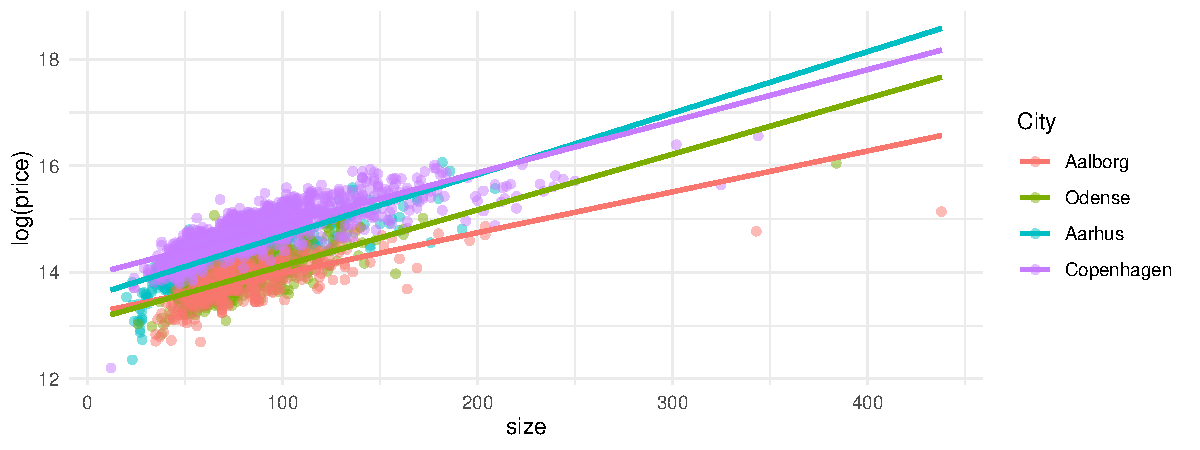
\includegraphics[width = 1\textwidth]{figures/Nanna/Forskellig_haelding.pdf}
    \caption{The lines represent linear regressions where \textit{log(price)} is treated as the dependent variable and $size$ in square meters is the independent variable.}
    \label{fig:Forskellig_haeldning}
\end{figure}
Making linear models for each of these groups, we find that the difference in slope between the models is significant.
For now this is simply seen from the figure \ref{fig:Forskellig_haeldning} and the coefficients in table \ref{tab:my-table}.
The term significance will be explored in more detail in section \ref{sec:Hypothesis_Testing}. 


\begin{table}[H]
\centering
\begin{tabular}{lrrrrrrr}
\toprule
\textbf{City}                                                                                       & \textbf{term}                & 
\textbf{estimate}            & \textbf{std.error}           & \textbf{statistic}           & \textbf{p.value}             \\
\midrule
Aarhus                                                                                & (Intercept)                  & 13.5                      & 0.0257                       & 527                         & 0                      \\
Aarhus                                                                            &  \textit{size}                   & 0.0115                       & 0.000325                         & 35.5                         & 1.24e-163                    \\
\addlinespace
Odense                                                                            &  (Intercept)                  & 13.1                     & 0.0310                       & 421                        & 0                    \\
Odense                                                                             &  \textit{size}                   & 0.0105                       & 0.000379                         & 27.7                        & 3.99e-105                    \\
\addlinespace
Aalborg                                                                           &  (Intercept)                  & 13.2                      & 0.0378                       & 350                         & 0                     \\
Aalborg                                                                            &  \textit{size}                   & 0.00766                       & 0.000425                         & 18.0                         & 1.14e- 53                    \\
\addlinespace
Copenhagen                                                                     &  (Intercept)                  & 13.9                      & 0.0196                       & 709.                        & 0                      \\
Copenhagen                                                                       &  \textit{size}                   &  0.00968                       & 0.000206                         & 47.1                        & 5.23e-273 \\                          
\bottomrule
\end{tabular}
\caption{Summary for the linear models $\log(price) \sim size$ in figure \ref{fig:Forskellig_haeldning}.}
\label{tab:my-table}
\end{table}

Adding \textit{city} as a parameter therefore decreases accuracy, and it might be wise to make separate models for each of the cities. 
Note that this example only considers the size, and not the other categorical variables.

% Below in figure \ref{fig:Opfoerelsesaar_plot} is a plot of how the parameter \textit{year.construct} influences \textit{price}.
% As reflected by the $R$-squared value seen in table \ref{tab:r-squared}, \textit{price} varies significantly depending on \textit{year.construction}.
% We thereby conclude that this parameter is important and should be included in the model. 

% \begin{figure}[H]
%     \centering
%     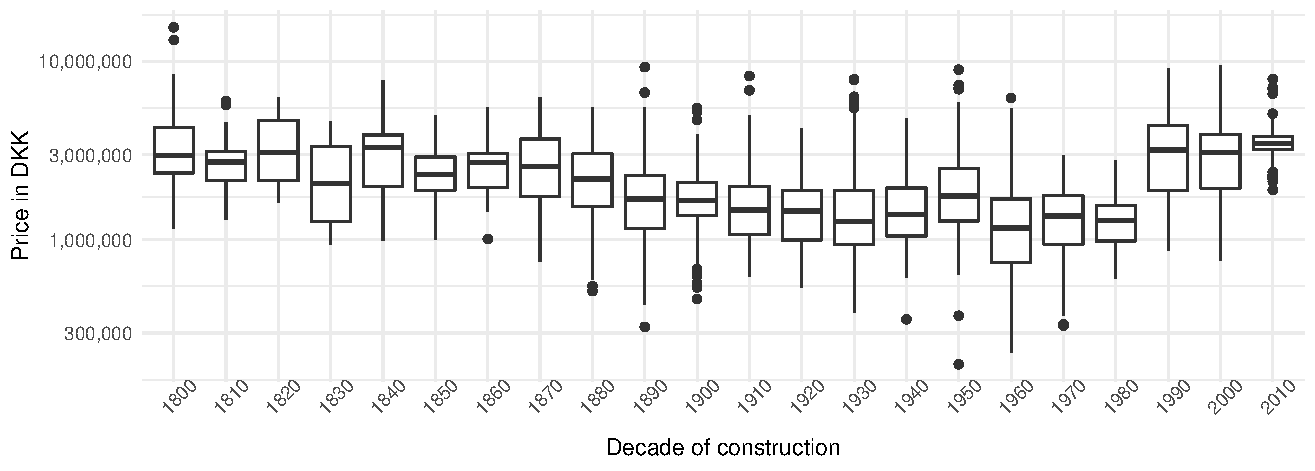
\includegraphics[width = 1\textwidth]{figures/Nanna/Opfoerelsesaarplot.pdf}
%     \caption{}
%     \label{fig:Opfoerelsesaar_plot}
% \end{figure}

From figure \ref{fig:Forskellig_haeldning} we see that the observations are heteroskedastic and their variance increases as \textit{size} increases. 
In order to satisfy the Gauss-Markov assumptions the observations need to have constant variance and we therefore need to transform the data, to remedy this. 
The logarithm is a variance stabilizing function, so using this on both \textit{price} and \textit{size} we see that the residuals seem to be approximately normally distributed around the regression line, as illustrated in figure \ref{fig:Log_Model_plot}. 

\begin{figure}[H] 
    \centering
    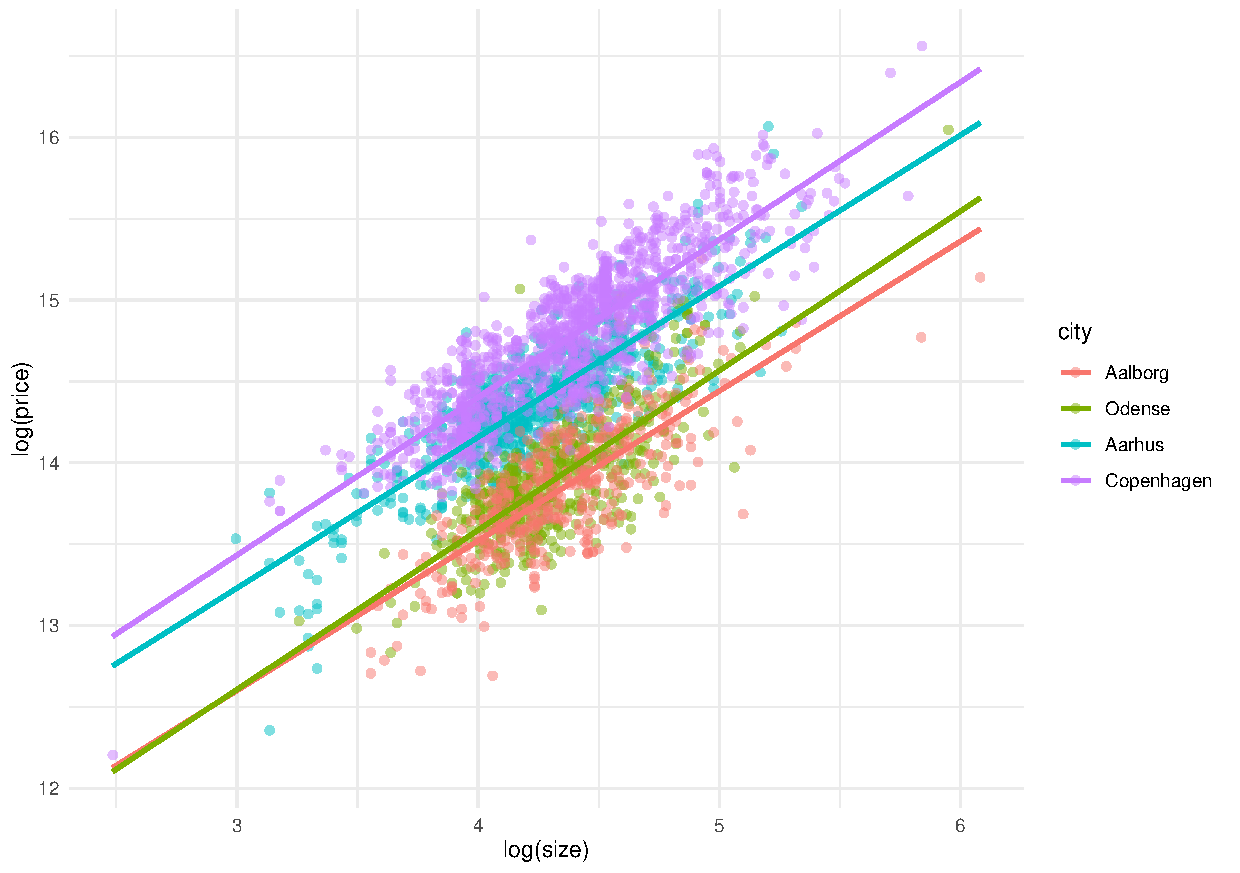
\includegraphics[width = 1\textwidth]{figures/Nanna/Plot_forskellig_haeldning.pdf}
    \caption{Simple linear regression model with $\log(price)$ as dependent variable and $\log(size)$ as the independent variable.}
    \label{fig:Log_Model_plot}
\end{figure}

In the same manner we conclude, that the variance of the price is less heteroskedastic after the log transformation, for all the independent variables listed in the model.
% Now that the model has been separated into 4 models, one for each city, table \ref{tab:r-squared} is no longer valid.
% The new models R-squared are presented in table \ref{tab:r-squared_4models}.

% \begin{table}[H]
% \centering
% \footnotesize
% \begin{tabular}{lrrrrrrrr}
% \toprule
% \textbf{}          & \textit{cond} & \textit{size} & \textit{selling.period} & \textit{year.construct} & \textit{balcony} & \textit{renovation}  & \textit{year.sale} \\
% \midrule
% $R^2_{Chp}$ & 0.112                & 0.6912              & 0.0007169           & 0.01179                  & 0.08983        & 0.01751      & 0.1021     \\
% $R^2_{Aar}$ & 0.05409                & 0.6368              & 8.675e-05           & 0.009992                  & 0.05901        & 0.0006814        & 0.06073 \\
% $R^2_{Ode}$ & 0.003955                & 0.6851              & 0.01061           & 0.02866                  & 0.004361        & 0.001168              & 0.003028 \\
% $R^2_{Aal}$ & 0.003904                & 0.5104              & 0.001361           & 0.002269                  & 0.02415        & 0.003244              & 0.05763 \\
% \bottomrule
% \end{tabular}
% \caption{\textit{R}-squared and adjusted \textit{R}-squared for the independent variables.}
% \label{tab:r-squared_4models}
% \end{table}
% As predicted, the $R$-squared for size are larger, when splitting the model up into 4, allowing for better model fit.
% Of note is the parameter $cond$ for Copenhagen, since this went from 0.001731 to 0.112, making it a much more useful parameter. 
Further, we will use the following model as our full model, in the coming sections.
\begin{align*}
    \log(price) \sim \log(size) + year.sale + \textit{cond} +  \textit{balcony}.
\end{align*}

\subsection{Multicollinearity}
As it was explained in section \ref{sec:consequence_of_hetero}, we desire as little multicollinearity as possible, as it increases the variance of the slope coefficients.
One way to quantify multicollinearity is
to use the variance inflation factor (VIF) which is defined as
\begin{align*}
    \text{VIF}_j = \frac{1}{1 - R^2_j}.
\end{align*}
The VIF can be interpreted as one of the three factors that inflates the variance of the slope coefficients, hence the name.
Performing regression for the 2 non-dummy variables yields the VIF's displayed in table \ref{tbl:vif}.
\begin{table}[H]
    \centering
    \begin{tabular}{lrrrr}
        \toprule
        & \multicolumn{4}{c}{\textbf{VIF}} \\
        \midrule
        \textbf{Variable} & \textbf{Copenhagen} & \textbf{Aarhus} & \textbf{Odense} & \textbf{Aalborg} \\
        \midrule
        $\log(size)$                & 1.078182 & 1.067156 & 1.020253 & 1.022091 \\
        $balcony$                   & 1.167294 & 1.071244 & 1.010425 & 1.021054 \\
        % $cond(medium)$              & 5.195332 & 9.506274 & 44.16799 & 11.06534 \\
        % $cond(high)$                & 5.330074 & 9.586961 & 44.30732 & 11.02007 \\
        % $year.sale(crisis)$         & 1.422332 & 1.275421 & 1.479368 & 1.287134 \\
        % $year.sale(post.crisis)$    & 1.572893 & 1.308654 & 1.570689 & 1.264966 \\
        \bottomrule
    \end{tabular}
    \caption{VIF's for the non-dummy variables.}
    \label{tbl:vif}
\end{table}
Generally we have small values, and
% however for the dummy variables $cond(medium)$ and $cond(high)$ the VIF's are larger.
% As suggested in \cite{Allison2012}, we can ignore high VIF's for dummy variables that represent a categorical variable with three or more categories.
% These dummy variables will have high VIF's even though they are not associated with other variables in the regression model.
thus we conclude that for all cities the VIF's are at most 1.167294 which corresponds to an $R$-squared of approximately 0.143318, which we deem below our threshold for multicollinearity.
One should also be cautious how much weight is put on multicollinearity.

It is clear that other things equal we want lower multicollinearity as this will reduce the variance of the slope coefficients given in \eqref{eq:slope_variance_OLS_estimator}.
But multicollinearity, or VIF, is only one of three components in the slope coefficient variance.
The other two being $\sigma^2$, the variance of the error term, and the total sample variation in $\textbf{x}_j$ given as $\text{SST}_j = \sum_{i=1}^n(x_{ij} - \overline{x}_j)$.
So before putting to much weight on a high VIF, one must also consider the other two factors with influence on the variance of the slope coefficients.
\chapter{Hypothesis Testing}
\label{ch:hypothesis_testing}
\section{Hypothesis Testing}\label{sec:Hypothesis_Testing}
In this section $t$-tests and $F$-tests are introduced to test the significance of the different parameters, both individually and combined, considered in our model. 

As an addition to the Gauss-Markov assumptions from chapter \ref{ch:Multip_linear_regresssion} we will introduce the following assumption, that imposes an additional restriction on the errors. 
\begin{assumption}[Normality of Errors] \label{as:normality_of_errors}
    Conditional on $\mathbf{X}$, the $\varepsilon_i$ are independent and identically distributed as $N(0, \sigma^2)$. Equivalently, $\boldsymbol{\varepsilon}$ given $\mathbf{X}$ is distributed as multivariate normal with mean zero and variance-covariance matrix $\sigma^2 \mathbf{I}_{n}$, i.e. $\boldsymbol{\varepsilon} \sim N_n(\mathbf{0}, \sigma^2 \mathbf{I}_{n})$.
\end{assumption}

\subsection{\textit{t}-test}
One way to test hypotheses about single parameters in the true regression model is to make use of the $t$-test. 
A $t$-test is an inferential statistic determining whether or not there is a significant difference between two t statistics, e.g.$\!$ the means of two groups, is significant. First we need a definition.

\begin{definition}[\textit{t}-distribution]\label{def:t_distribution}
    Let $Z \sim N(0,1)$ and $W \sim \chi^2(n)$ be independent. Then the random variable
    \begin{align*}
       T = \frac{Z}{\sqrt{W/n}}
    \end{align*}
    has a $t$-distribution with $n$ degrees of freedom and is denoted $T \sim t(n)$.
\end{definition}

The $pdf$ of the $t$-distribution has a shape that is similar to the standard normal distribution. 
Except that it is more spread out and thus has larger areas in the tails. 
In figure \ref{fig:t_distribution} the $pdf$ of the $t$-distribution is plotted for various degrees of freedom compared to the standard normal distribution. 

\begin{figure}[H]
    \centering
    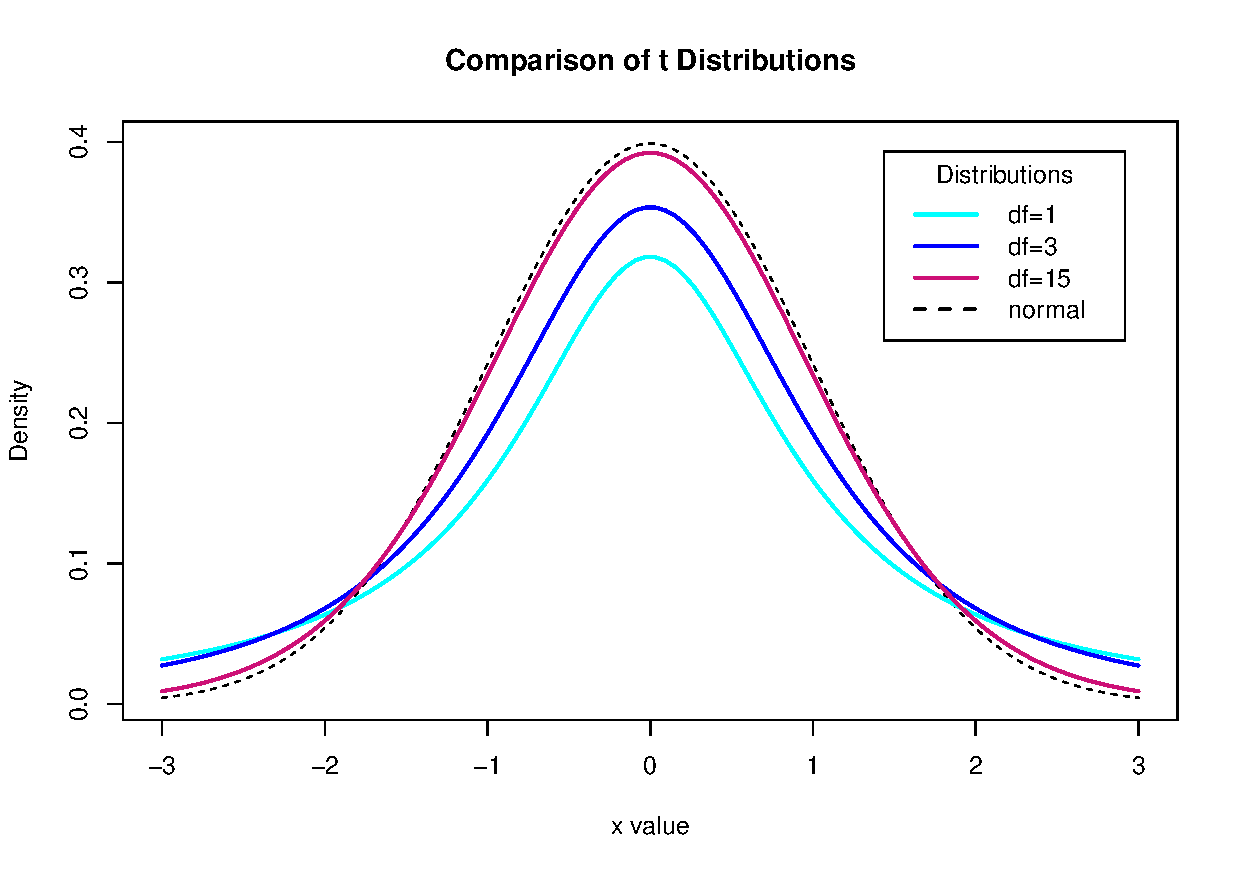
\includegraphics[width = 0.8\textwidth]{figures/t_distribution.pdf}
    \caption{The $t$-distribution for various degrees of freedom compared to the standard normal distribution.}
    \label{fig:t_distribution}
\end{figure}

Clearly, as the degrees of freedom increases, the $t$-distribution approaches the standard normal distribution, so $t(n) \rightarrow N(0,1)$ for $n\rightarrow \infty$. This also follows from the Central Limit Theorem, presented later in this chapter in theorem \ref{th:Central_limit_theorem}. 

Recall that OLS produces unbiased estimates c.f.$\!$ theorem \ref{th:unbiasedness_of_ols}, let $d_j=(\textbf{X}^\top\textbf{X})^{-1}_{jj}$ denote the $j$'th diagonal element of $(\textbf{X}^\top \textbf{X})^{-1}$, let $\hat{\beta}_j(\textbf{y})$ denote the $j$'th coordinate of the OLS estimate $\betahat(\textbf{y})$ and $s^2(\textbf{y})$ denote the unbiased estimate for $\sigma^2$ found in \eqref{eq:unbiased_variance_estimate}.

\begin{definition} [$t$-statistic] \label{def:t-test}
    Let $\beta_{0j}$ be given and consider the hypothesis $\mathcal{H}_0 \ : \ \beta_j=\beta_{0j}$. 
    The $t$-statistic for $\mathcal{H}_0$ is then given by
\begin{align}\label{eq:t_test1}
   t_j(\textbf{y};\beta_{0j}) = \frac{\hat{\beta}_j - \beta_{0j}}{\sqrt{d_j s^2(\textbf{y})}} \quad \text{for} \quad j=0,\ldots,k
\end{align}
where large values of $|t_j(\textbf{y};\beta_{0j})|$ are critical for $\mathcal{H}_0$.
\end{definition}

In order to construct a hypothesis test, the following result is needed.

\begin{theorem} [Test of Individual Parameters] \label{th:t_distribution}
Let the situation be as in definition \ref{def:t-test}. Under $\mathcal{H}_0 \ : \ \beta_j=\beta_{0j}$ we have 
\begin{align}
   t_j(\textbf{y};\beta_{0j})  \sim t(n-k-1) \quad \text{for} \quad j=0,\ldots,k
\end{align}
and the $p$-value is
\begin{align}\label{eq:t_test_pvalue}
    p(\textbf{y},\beta_{0j})=P\Big(|t_j(\textbf{Y};\beta_{0j})|\geq |t_j(\textbf{y};\beta_{0j})|\Big).
\end{align}
The $p$-value is the probability that, if the null hypothesis were true, sampling variation would produce an estimate that is further away from the hypothesised parameter value than our data estimates.  
Thus it would lie in the tails of the $pdf$ of the $t$-distribution seen in figure \ref{fig:t_distribution}.
Meaning that a low $p$-value is evidence against $\mathcal{H}_0$.

Furthermore, for $0<\alpha<1$, using the $t$-test at level $\alpha$, the limits of a ($1-\alpha$)-confidence interval for $\beta_j$ is
\begin{align} \label{eq:t_statistic}
    \hat{\beta}_{j}(\textbf{y}) \pm t_{1-\alpha/2}(n-k-1)\sqrt{d_j s^2(\textbf{y})}
\end{align}
which corresponds to the cases where we accept the hypothesis that $\beta_j$ takes a specific value.
\end{theorem}
\begin{proof}
We want to verify that \eqref{eq:t_test1} has a $t$-distribution. Recall due to the assumptions \ref{as:linear_in_the_parameters}, \ref{as:no_perfect_collinearity}, \ref{as:zero_conditional_mean}, \ref{as:homoskedasticity_and_no_serial_correlation} and \ref{as:normality_of_errors} example \ref{ex:MLE_for_model} showed that

\begin{align} \label{eq:th_t_test}
    \hat{\betabold}(\textbf{Y}) \sim N_k(\betabold,\sigma^2(\textbf{X}^T\textbf{X})^{-1})
\end{align}
which entails
\begin{align*}
    &\hat{\beta}_j(\textbf{Y})\sim N(\beta_j , \sigma^2d_j) \
    \Leftrightarrow \  (\hat{\beta}_j(\textbf{Y})-\beta_j) \sim N(0,\sigma^2d_j)
\end{align*}
and standardizing is done by dividing by the standard deviation, so
\begin{align*}
    (\hat{\beta}_j(\textbf{Y})-\beta_j)/\sqrt{d_j\sigma^2} \sim N(0,1).
\end{align*}
The distribution of $s^2$ comes from \eqref{eq:eq:unbiased_variance_estimate}, so
\begin{align} \label{eq:sigma_square_of_Y}
    s^2(\textbf{y}) = \dfrac{1}{(n-k-1)}\sum_{i=1}^n \hat{\varepsilon}_i^2
\end{align}
which is a sum of squared independent normally distributed random variables and therefore
\begin{align*}
s^2(\textbf{Y}) \sim \sigma^2 \chi^2(n-k-1)/(n-k-1).    
\end{align*}
We will now show that
\begin{align*}
    (\hat{\beta}_j(\textbf{Y})-\beta_j)/\sqrt{d_j\sigma^2} \sim N(0,1) \quad \text{and} \quad s^2(\textbf{Y}) \sim \sigma^2\chi^2 (n-k-1)/(n-k-1)
\end{align*}
are independent.
The independence of $s^2(\textbf{Y})$ and $\betahat$ is seen as $\betahat$ and $\textbf{r}(\textbf{y}) = \textbf{y} -\textbf{X} \betahat$ are independent, which will be explained in detail below.
Consider
\begin{align*}
    \textbf{r}(\textbf{y}) = \textbf{y}-\textbf{X} \betahat = \textbf{y} - \textbf{H} \textbf{y} = (\textbf{I}-\textbf{H})\textbf{y} = (\textbf{I}-\textbf{H}) (\textbf{X} \betahat + \epsilonhat) = (\textbf{I} - \textbf{H}) \epsilonhat.
\end{align*}
It is seen that $E(\epsilonhat) = \textbf{0}$ by assumption \ref{as:normality_of_errors}. 
Now the expected value of the product $\textbf{r}(\textbf{y}) \betahat^\top$ is calculated, in order to later calculate the covariance
\begin{align} \label{eq:Variance_of_product}
    E(\textbf{r}(\textbf{y}) \betahat^\top) &= E \left( [(\textbf{I} - \textbf{H}) \epsilonhat] [(\textbf{X}^\top \textbf{X})^{-1} \textbf{X}^\top \textbf{y}]^\top \right) \nonumber \\
    &= E \left( [(\textbf{I}-\textbf{H}) \epsilonhat] \textbf{y}^\top \textbf{X} (\textbf{X}^\top \textbf{X})^{-1} \right) \nonumber \\
    &= (\textbf{I}-\textbf{H}) E(\epsilonhat \textbf{y}^\top ) \textbf{X}(\textbf{X}^\top \textbf{X})^{-1}. 
\end{align}
For clarity we take out the term $E(\epsilonhat \textbf{y}^\top )$ and calculate it separately
\begin{align*}
    E \left[ \epsilonhat \textbf{y}^\top \right] &= E \left[ \epsilonhat (\epsilonhat^\top + \betahat^\top \textbf{X}^\top) \right] \\
    &= E \left[ \epsilonhat \epsilonhat^\top + \epsilonhat \betahat^\top \textbf{X}^\top \right] \\
    &= E[\epsilonhat \epsilonhat^\top]
\end{align*}
This is equal to the variance of $\epsilonhat$ since $\var(\epsilonhat) = E(\epsilonhat \epsilonhat^\top) - E(\epsilonhat)E(\epsilonhat)^\top$, where $E(\epsilonhat)=\textbf{0}$.
This is by assumption \ref{as:normality_of_errors} equal to $\sigma^2 \textbf{I}_n$.
Inserting this into \eqref{eq:Variance_of_product} yields
\begin{align*}
    \sigma^2 (\textbf{I}-\textbf{H}) \textbf{X} (\textbf{X}^\top \textbf{X})^{-1} = \textbf{0}
\end{align*}
because
\begin{align*}
    (\textbf{I}-\textbf{H})\textbf{X} &= (\textbf{I}-\textbf{X}(\textbf{X}^\top \textbf{X})^{-1}\textbf{X}^\top)\textbf{X} \\
    &= \textbf{X} - \textbf{X} (\textbf{X}^\top \textbf{X})^{-1} (\textbf{X}^\top \textbf{X}) \\
    &= \textbf{X} - \textbf{X} = \textbf{0}
\end{align*}
Therefore the covariance and by extension correlation is
\begin{align*}
    \cov (\betahat, \textbf{r}(\textbf{y})) &= E(\betahat\textbf{r}(\textbf{y})^\top) - E(\betahat) E(\textbf{r}(\textbf{y}))^\top \\
    &= \textbf{0} - E(\betahat) \cdot \textbf{0}
\end{align*}
Assuming that they are multivariate normally distributed, this means that $\betahat$ and $s^2(\textbf{Y})$ are independent, since $s^2(\textbf{Y})$ is just a constant times $SSR$ c.f.$\!$ \eqref{eq:sigma_square_of_Y}.

We see that
\begin{align*}
    \frac{s^2(\textbf{Y})}{\sigma^2(\textbf{Y})} \sim \chi^2(n-k-1)/(n-k-1)
\end{align*}
and with use of definition \ref{def:t_distribution} we obtain that
\begin{align*}
    t_j(\textbf{Y};\beta_j)=\frac{(\hat{\beta}_j(\textbf{Y})-\beta_j)/\sqrt{d_j\sigma^2(\textbf{Y})}}{\sqrt{d_js^2(\textbf{Y})/d_j\sigma^2}} \sim t(n-k-1)
\end{align*}
and hence the first part of the theorem composed of \eqref{eq:th_t_test} is verified, and second part follows immediately. 
\end{proof}

In the case of testing OLS estimates, we usually test the special case where the estimates are anything other than zero. In this case, we test against the two-tailed alternatives and therefore the primary interest is testing the null hypothesis
\begin{align} \label{eq:t_test_h0}
    \mathcal{H}_0:\beta_j=0.
\end{align}
In this case the alternative hypothesis is
\begin{align} \label{eq:t_test_ha}
    \mathcal{H}_1 : \beta_j \neq 0,
\end{align}
which means, that $\textbf{x}_j$'s effect on the expected value $\textbf{y}$ can be both positive or negative.
Since after controlling for all other independent variables than $\textbf{x}_j$, $\beta_j$ measures the partial effect of $\textbf{x}_j$ on the expected value of $\textbf{y}$. 
Thus \eqref{eq:t_test_h0} means that, after $\textbf{x}_1,\textbf{x}_2, \ldots, \textbf{x}_{j-1}, \textbf{x}_{j+1}, \ldots, \textbf{x}_k$ have been accounted for, $\textbf{x}_j$ has no effect on the expected value for $\textbf{y}$ since $\beta_j=0$. 
For $\textbf{x}_j$ having a partial effect on the expected value of $\textbf{y}$, the value of $\beta_j$ has to be anything other than zero.

In practice, $\hat{\beta}_j$ will rarely be zero, whether or not $\mathcal{H}_0$ is true.
Therefore the question is rather how to determine how far $\hat{\beta}_j$ is from zero. 
The further the sample value of $\hat{\beta}_j$ is from zero, the bigger is the evidence against $\mathcal{H}_0$. 
However, the larger the standard error is of $\hat{\beta}_j$, the smaller is the evidence against $\mathcal{H}_0$. 
Thus $t_{j}$ is a ratio of how many estimated standard deviations $\hat{\beta}_j$ is away from zero.
In general the larger value of $t_{j}$, the larger the evidence against $\mathcal{H}_0$. 
The precise rule for rejecting $\mathcal{H}_0$ depends on the alternative hypothesis and the chosen significance level.
The $t$-value in \eqref{eq:t_statistic} is found using the inverse of the \textit{cdf} of the $t$-distribution with $(n - k - 1)$ degrees of freedom evaluated in $(1-\alpha/2)$. 
Since the $t$-distribution is symmetric, $\pm t_{1-\alpha/2}$ is the same as $\mp t_{\alpha/2}$.

\subsubsection{Application of \textit{t}-test}  \label{ex:ttest}
Consider the simple model with one independent variable for each of the cities 
\begin{align*}
    \log(price) \sim \log(size).
\end{align*}
The test is two-tailed, therefore we test the null hypothesis $\mathcal{H}_0:\beta_1=0.$
We complete the $t$-test at significance level $\alpha=0.05$ which gives the limits of a 95\%-confidence interval for $\hat{\beta}_1$.
We obtain the estimated model for Copenhagen with values listed in the following table.

\begin{table}[H]
\centering
\begin{tabular}{lrrrr}
\toprule
\textbf{term} & \textbf{estimate} & \textbf{std.error} & \textbf{t value} & \textbf{p.value}\\
\midrule
(Intercept) & 10.52852 & 0.07412 & 142.05 & <2e-16\\
$\log(size)$ & 0.96832 & 0.01682 & 57.59 & <2e-16\\
\bottomrule
\end{tabular}
\caption{Summary for the regression $\log(price) \sim \log(size)$ for Copenhagen.}
\end{table}

In order to calculate the $t$-value of $\hat{\beta}_1$ we define the values in \eqref{eq:t_test1}:
\begin{lstlisting}
#We define some useful values according to our definition and theorem
n <- 1182 ; k <- 1
beta_hat <- 0.96832 ; beta_null <- 0
df <- n - (k + 1)
x <- c(rep(1, n), log(Copenhagen$size)); X <- matrix(data = x, nrow = n)
y <- c(log(Copenhagen$price))
d <- solve((t(X) %*% X)) ; d_j <- d[2,2]
fitted <- X %*% solve(t(X) %*% X) %*% t(X) %*% y
sigma_hat2 <- sum((y - fitted)^2)/(n-2)
std_error <- (sqrt(d_j*sigma_hat2))
\end{lstlisting}
Now we can calculate the $t$-value by inserting the obtained values in \eqref{eq:t_test1}.
\begin{lstlisting}
#t-statistic
t_stat <- (beta_hat-beta_null)/std_error; t_stat
[1] 57.58523
\end{lstlisting}
and the p value by inserting the obtained values in \eqref{eq:t_test_pvalue}.
\begin{lstlisting}
#p-value
p_val <- pt(t_stat, df = df, lower.tail = FALSE)*2; p_val
[1] 0
\end{lstlisting}
The parameter $\hat{\beta}_1=0.96832$ has $t$-value $t_1 = 57.58523$ which is significant because of the low $p$-value. 
Therefore we reject the null hypothesis at a $5\%$-significance level. 
This is illustrated in figure \ref{fig:t_distributionplot1}, where the dotted lines illustrates the respective end and beginning of the the rejection regions.
In the figure it is clear, that we are far into the tail of the null distribution which also indicates a small $p$-value. 
This indicates, that our observed $\hat{\beta}_1$ is more extreme than what is reasonably expected if the null hypothesis were true.
\begin{figure}[H]
    \centering
    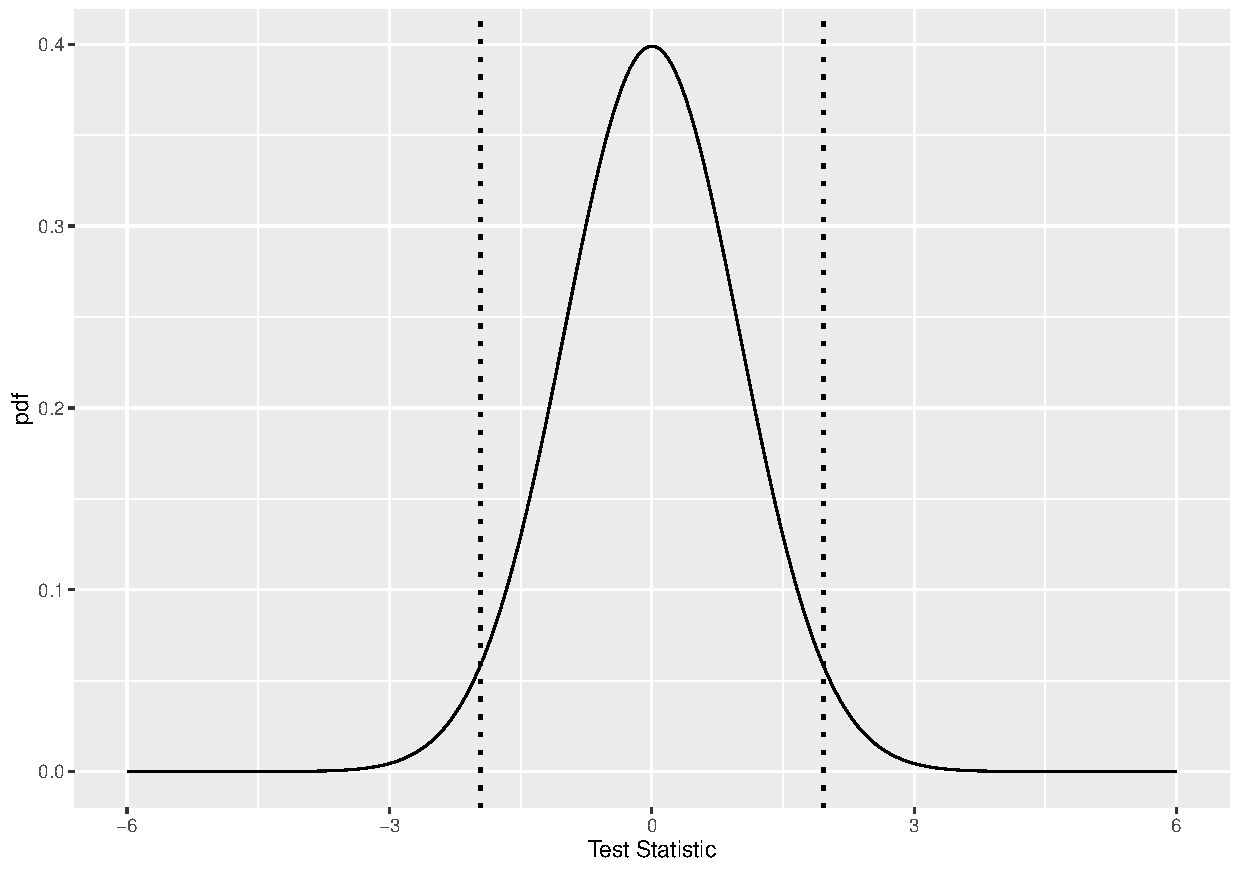
\includegraphics[width = 0.6  \textwidth]{figures/Nanna/t_distribution123.pdf}
    \caption{5 \% rejection rule for $\mathcal{H}_1:\beta_1\neq0$ with 1180 degrees of freedom. The $t$ value of the observed value $\hat{\beta}_1=0.96832$ is far out in the tail to the right.}
    \label{fig:t_distributionplot1}
\end{figure}
The critical $t$-values for $\mathcal{H}_0$ is found by the inverse of the $cdf$ where we obtain the $t$-values of chosen probabilities. 
The $95\%$-significance level, means that we evaluate the inverse $cdf$ in $0.025$ and $0.975$. 
This is illustrated in figure \ref{fig:CDF_inverse} where the intersection of the dotted lines gives the critical $t$-values.
\begin{figure}[H]
    \centering
    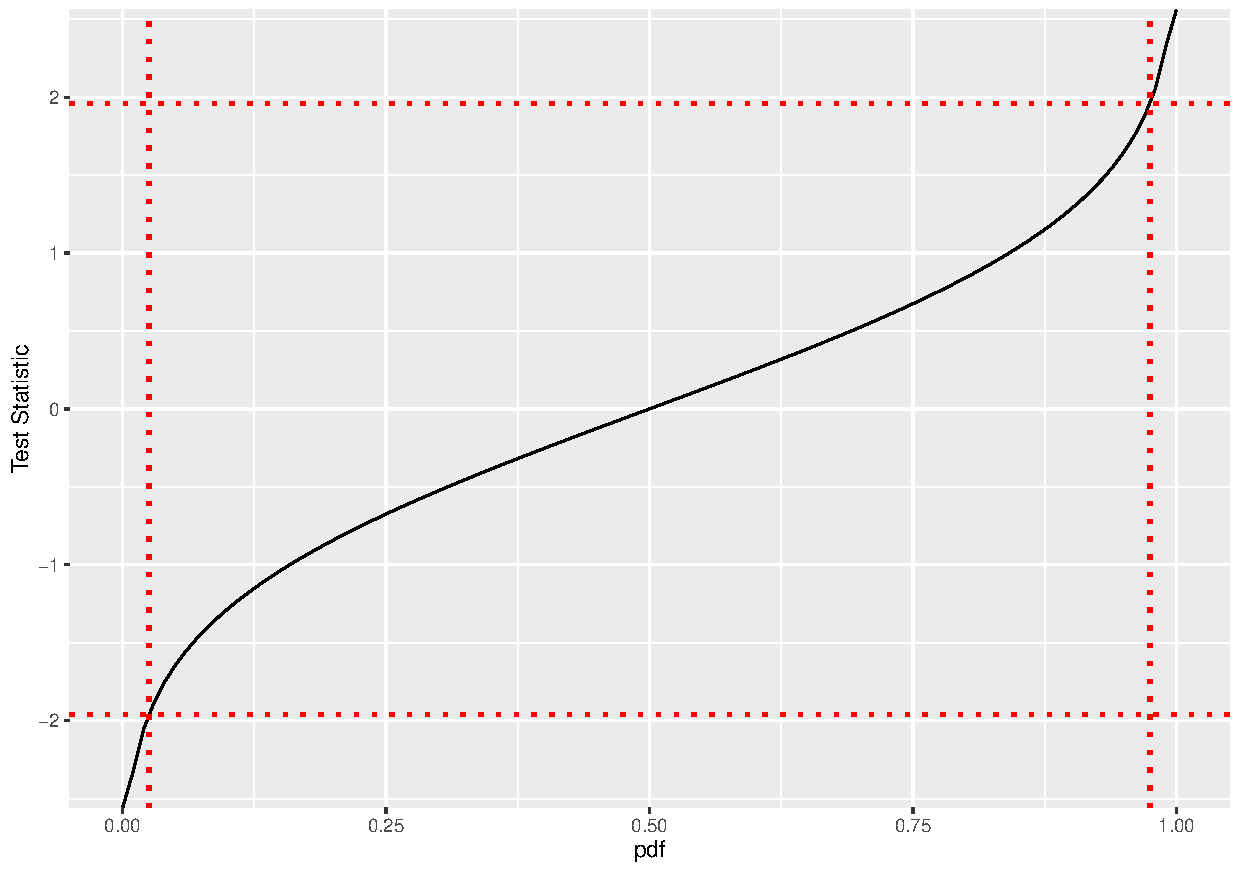
\includegraphics[width = 0.6\textwidth]{figures/Nanna/Inverse_CDF.pdf}
    \caption{The inverse $cdf$ in which we obtain the critic values for $\mathcal{H}_0$ of the chosen $95\%$-significance level.}
    \label{fig:CDF_inverse}
\end{figure}
Now we have concluded, that $\log(size)$ has a statistically significant effect on $\log(price)$ at a 95\%-confidence level for Copenhagen. 
By computing the limits of a 95\%-confidence interval for $\hat{\beta}_1$ with \eqref{eq:t_statistic}, we find the 95\%-confidence interval which we expect contains the ``true'' parameter.
\begin{lstlisting}
#We calculate the confidence interval for our parameter
beta_hat+std_error*qt(0.975, df = df)
[1] 1.001311
beta_hat+std_error*qt(0.025, df = df)
[1] 0.9353285
\end{lstlisting}
Note that the confidence interval for $\betahat_1$ does not contain 0, as expected.
From this lower and upper bound of the confidence intervals of the parameters, we can plot the area in which we expect the ``true'' line to be. 
In figure \ref{fig:t_distributionplot2} the blue line is our estimated model and the shaded area is the 95\%-confidence interval of the model. 
\begin{figure}[H]
    \centering
    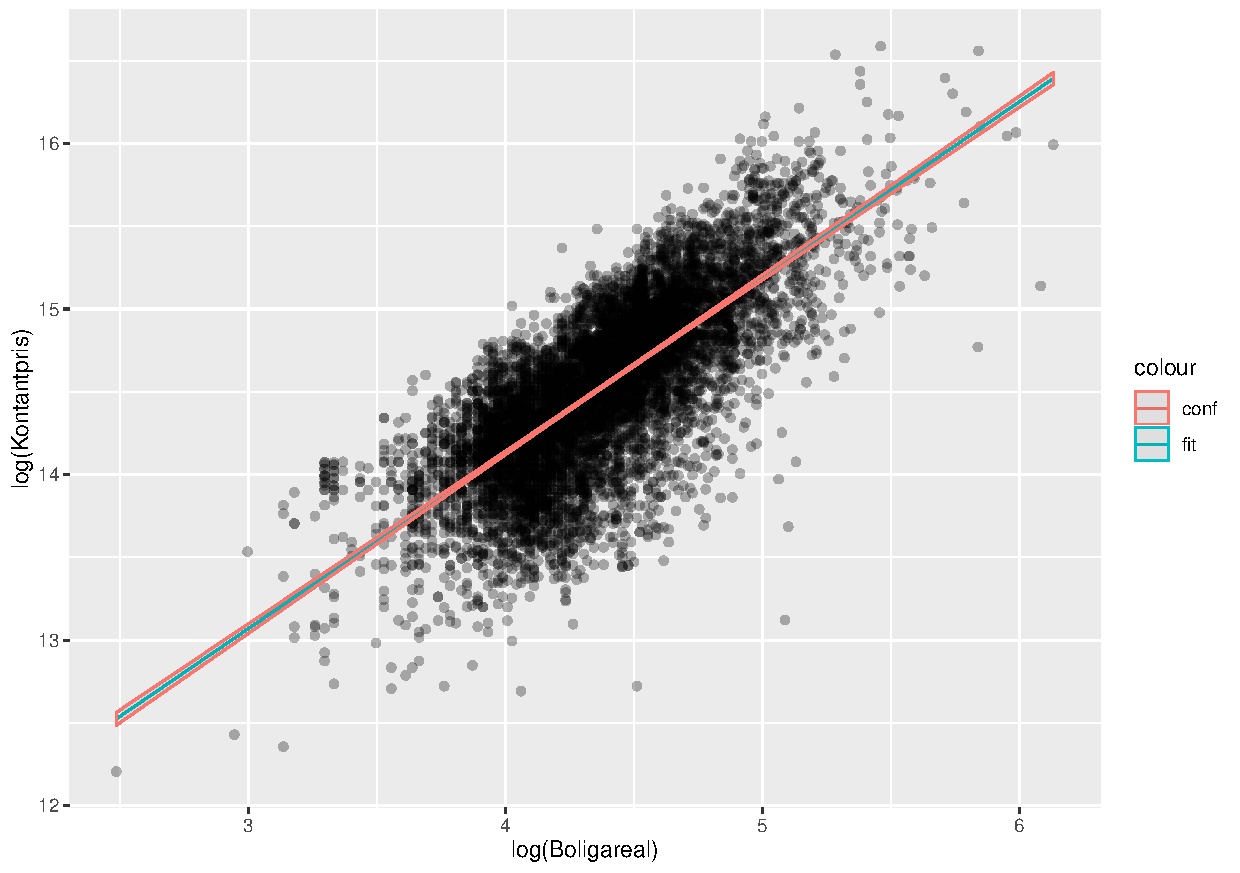
\includegraphics[width = 0.7\textwidth]{figures/Nanna/Confidence_interval.pdf}
    \caption{Plot of the observed values, the fitted regression line and its $95\%$-confidence intervals in which we expect the ``true'' line to be.}
    \label{fig:t_distributionplot2}
\end{figure}

For the remaining cities, we draw the same conclusions. 
Each of the simple models of the cities gives $t$-statistics that entails significant $p$-values and we can reject the null hypothesis in all cases. 
Therefore, we conclude that $\log(size)$ has a statistically significant effect on $\log(price)$ at a 95\%-confidence level in Copenhagen, Aarhus, Odense and Aalborg. 

We have performed $t$-test for each of the parameters presented in section \ref{sec:modelling} for each of the four cities. As a result, \textit{balcony} and \textit{year.sale} are also significant for each of the four cities. 
Varying results are obtained for the remaining parameters, which indicates, that different parameters determine the price for each city. The parameter \textit{cond} is also significant for Copenhagen but only for the value ``high''. 

From the $t$-test, we have obtained knowledge of the parameters individual effect on $\log(price)$ and if the effect is considered as significant. 
In order to test models with more than one parameter, we therefore introduce the $F$-test as a method.

% \section{Confidence intervals}

% \begin{definition} [The (1-$\alpha$)-confidence Region]
% \label{def:confidence_region}
% Suppose that for a given number $\alpha \in (0,1)$ and for each $\textbf{y} \in \mathcal{Y}$, we have specified a subset $A(\textbf{y})$ of the parameter space $\Theta^k$, such that
% \begin{align*}
%     P_{\boldsymbol{\beta}} (\boldsymbol{\beta} \in A(\textbf{Y})) = 1 - a, \quad \forall \boldsymbol{\beta} \in \Theta^k
% \end{align*}
% Then we call $A(y)$ a $(1-\alpha)$-confidence region for $\boldsymbol{\beta}$.
% \end{definition}

% If the parameter is one-dimensional $(k=1)$ and the observations, $y$ are normally distributed, then the confidence region become the interval

% \begin{align*}
%     \left[ 
%     \hat{\beta}(\textbf{y}) + \Phi_{\alpha/2} \sqrt{D(\hat{\beta}(\textbf{y})} , \hat{\beta}(\textbf{y}) + \Phi_{1 - \alpha/2} \sqrt{D(\hat{\beta}(\textbf{y})}
%     \right]
% \end{align*}

% for $0 < \alpha \leq 0.5$. 


% \begin{example}
% Consider again the situation from example \ref{ex:model1}. By theorem \ref{th:distribution_ml_estimator} the asymptotic distribution of the ML estimator is given by
% \begin{align*}
%     \betahat \rightarrow^\mathcal{D} N\left( \mathbf{ \beta }, \boldsymbol{i}(\betahat)^{-1} \right)
% \end{align*}
% Since $\mathbf{\beta}$ is one-dimensional, $k=1$, and for $0\leq \alpha \leq 0.5$ we have the approximate $(1-\alpha)$-confidence interval
% \begin{align*}
% \left[ \betahat(\mathbf{y}) + \Phi_{\alpha/2} \sqrt{D\left( \betahat\left(\mathbf{y}\right)\right)}, \betahat(\mathbf{y}) + \Phi_{1 - \alpha/2} \sqrt{D\left( \betahat\left(\mathbf{y}\right)\right)} \right],
% \end{align*}
% where $D\left(\betahat(\mathbf{y})\right) = j\left(\betahat(\mathbf{y})\right)^{-1}$.
% For $\alpha=0.05$ we have the approximate $95\%$-confidence interval for $\mathbf{\beta}$:
% \begin{align*}
% \left[ \bar{y} - \frac{1.96}{\sqrt{n}}, \bar{y} + \frac{1.96}{\sqrt{n}} \right]    
% \end{align*}
% \end{example}

\subsection{\textit{F}-Test}\label{sec:Ftest}
Suppose we want to test if a multiple regression model has redundant explanatory variables.
In terms of hypothesis testing this is the null hypothesis: A set of variables has no statistically significant effect on $\textbf{y}$, once another set of variables has been controlled for.

Determining this will be done by analyzing the change in $SSR$, that is the difference in how well the models explain the variation in the data, and determining whether this change is significant. 
Suppose we have $model$ 1 with $(k+1)$ variables 
\begin{align*}
    \textbf{y} = \textbf{X}\betabold +\ \boldsymbol{\varepsilon},
\end{align*}
this is known as the unrestricted model. The restricted model or $model$ 0 lacks the $q$ variables, for which we want to check significance, that is
\begin{align*}
    \textbf{y} = \beta_0 + \beta_1 \textbf{x}_1 + \cdots + \beta_{k-q} \textbf{x}_{k-q} + \boldsymbol{\varepsilon}.
\end{align*}
Therefore $q$ is the difference in degrees of freedom between the two models.
This means we want to test the hypothesis
\begin{align}
    \mathcal{H}_0: \beta_{k-q+1} = \ldots = \beta_k = 0.
\end{align}
These are referred to as the exclusion restrictions. 
This is done using the $F$-statistic
\begin{align}\label{eq:F_statistic}
    F \equiv \frac{\| \textbf{H}_1 \textbf{y} - \textbf{H}_0 \textbf{y} \|^2/q}{\| \textbf{y} - \textbf{H}_1 \textbf{y} \|^2/(n-k-1)},
\end{align}
that is the relative increase in $SSR$, when going from $model$ 0 to $model$ 1. 
$\| \textbf{y} - \textbf{H}_0 \textbf{y} \|^2$ is the $SSR$ of $model$ 0 and $\| \textbf{y} - \textbf{H}_1 \textbf{y} \|^2$ is that of $model$ 1. 
$q$ is referred to as the numerator degrees of freedom, and $(n-k-1)$ is the denominator degrees of freedom. 

The change in $SSR$, when going from $model$ 0 to $model$ 1, is always non-negative because the model has more parameters to explain the data. 
This is discussed further in theorem \ref{th:Likelihood_ratio_linear_models}.

We will therefore reject $\mathcal{H}_0$, when $F$ is sufficiently large compared to the critical value, since this indicates that significantly more of the variation of the data has been explained by $model$ 1, as compared to $model$ 0.

As with the $t$-test, there is no correct significance level, but $\alpha = 0.05$ is often chosen. 
The critical value for the significance level can be determined by calculating one explicitly from the $cdf$ of the $F$-distribution found below see definition \ref{def:F-distribution}. 
This is equivalent to the procedure for $t$-test.

$\mathcal{H}_0$ is therefore rejected if the $F$-statistic is greater than the critical value
\begin{align*}
    F>c.
\end{align*}
If this is the case, the explanatory variables $\textbf{x}_{k-q+1}, \ldots, \textbf{x}_k$ are said to be jointly statistically significant. 
Otherwise they are said to be jointly insignificant, which can justify removing them from the model. 
In order to determine the critical value, the $F$-distribution is given.
\begin{definition}[$F$-Distribution]\label{def:F-distribution}
    Let $X_1 \sim \chi_{k_1}^2$ and $X_2 \sim \chi_{k_2}^2$ be independent random variables. Then the random variable 
        \begin{align*}
            F(k_1,k_2) = \frac{X_1/k_1}{X_2/k_2}
        \end{align*}
    has an $F$-distribution with $(k_1, k_2)$ degrees of freedom, which is denoted as $F(k_1,k_2) \sim F_{k_1, k_2}$.
\end{definition}
The $p$-value for the $F$-test is analogouse to that of the $t$-test
\begin{align*}
    p = P(F_{q,n-k-1} > F).
\end{align*}
That is the probability of observing this $F$-statistic under $\mathcal{H}_0$. 
The confidence level therefore reflects how sure we are that the model under $\mathcal{H}_0$ has generated the data.

\subsubsection{Equivalence of Tests}
The likelihood ratio can compare the goodness of fit for two models, specifically one over the entire parameter space and one with a restriction imposed.
It would therefore be interesting to see what relation it has to the $F$-test. 
Below it will be shown that the $F$-test is actually equivalent to the likelihood ration test.
This means that, going forward, we can just use the $F$-test to test joint significance for parameters.
Note this is only the case for multiple regression. 

\begin{theorem}[Likelihood Ratio For Linear Models]
\label{th:Likelihood_ratio_linear_models}
    The Likelihood ratio
    \begin{align*}
        \lambda(\textbf{y}) = \frac{\sup \ L(\textbf{y};\boldsymbol{\mu}_0, \sigma_0^2)}{\sup \ L(\textbf{y};\boldsymbol{\mu}_1, \sigma_1^2)}
    \end{align*}
    is a strictly decreasing function of $F(\textbf{y})$ under $\mathcal{H}_0$, such that
    \begin{align*}
        F(\textbf{Y}) \sim F_{q, n-k-1}.
    \end{align*}
\end{theorem}

\begin{proof}
    Under $\mathcal{H}_1$: $\boldsymbol{\mu}_1 = \textbf{H}_1 \textbf{y} \in \Omega_1$ and $\hat{\sigma}_1^2 = \frac{\| \textbf{y} - \textbf{H}_1 \textbf{y} \|^2}{n}$, the log-likelihood 
    function for the normal distribution is
    \begin{align*}
        l(\textbf{y};\boldsymbol{\mu}_1, \hat{\sigma}_1^2) &= -\frac{n}{2} log(\hat{\sigma}_1^2) - \frac{1}{2 \hat{\sigma}_1^2} \| \textbf{y} - \textbf{H}_1 \textbf{y} \|^2 \\
        &= -\frac{n}{2} log(\hat{\sigma}_1^2) - \frac{n}{2},
    \end{align*}
    and similarly for $\mathcal{H}_0:$ $\boldsymbol{\mu}_0 = \textbf{H}_0 \textbf{y} \in \Omega_0$. 
    Therefore the likelihood ratio can be written as
    \begin{align*}
        \lambda(\textbf{y}) &= \exp \left( l(\textbf{y};\boldsymbol{\mu}_0, \hat{\sigma}_0^2) - l(\textbf{y};\boldsymbol{\mu}_1, \hat{\sigma}_1^2) \right) \\
        &= \exp \left( -\frac{n}{2} \Big( log(\hat{\sigma}_0^2) - log(\hat{\sigma}_1^2)\Big) \right) \\
        &= \left( \frac{\| \textbf{y} - \textbf{H}_1 \textbf{y} \|^2}{\| \textbf{y} - \textbf{H}_0 \textbf{y} \|^2} \right)^{\frac{n}{2}} \\
        &= \left( \frac{\| \textbf{y} - \textbf{H}_1 \textbf{y} \|^2}{\| \textbf{y} - \textbf{H}_1 \textbf{y} \|^2 + \| \textbf{H}_1 \textbf{y} - \textbf{H}_0 \textbf{y} \|^2} \right)^{\frac{n}{2}}.
    \end{align*}
    The last equation holds because $\textbf{y} - \textbf{H}_1 \textbf{y}$ is orthogonal to $\Omega_1$ and $(\textbf{H}_1 \textbf{y} - \textbf{H}_0 \textbf{y}) \in \Omega_1$. 
    Dividing by the numerator and using \eqref{eq:F_statistic}, the above equation becomes
    \begin{align*}
        \lambda(\textbf{y}) &= \left( \frac{1}{1 + \frac{\| \textbf{H}_1 \textbf{y} - \textbf{H}_0 \textbf{y} \|^2}{\| \textbf{y} - \textbf{H}_1 \textbf{y} \|^2}} \right)^{\frac{n}{2}} \\
        &= \left( \frac{1}{1 + \frac{q}{n-k-1}F(\textbf{y})}  \right)^{\frac{n}{2}}.
    \end{align*}
    The likelihood ratio is therefore a function of the $F$-statistic, and since it is in the denominator, $\lambda(\textbf{y})$ is a decreasing function of $F(\textbf{y})$. We again see that large values of $F$ are critical, since small values of $\lambda(\textbf{y})$ are critical.
    
    The fact that $F$ is $F$-distributed is seen from
    \begin{align*}
        F(\textbf{Y}) &= \frac{\| \textbf{H}_1 \textbf{Y} - \textbf{H}_0 \textbf{Y} \|^2/q}{\| \textbf{Y} - \textbf{H}_1 \textbf{Y} \|^2/(n-k-1)} \\
        &= \frac{\| (\textbf{H}_1 - \textbf{H}_0) \textbf{Y} \|^2/q}{\| (\textbf{I} - \textbf{H}_1) Y \|^2/(n-k-1)} \\
        &\sim \frac{\chi^2(q)/q}{\chi^2(n-k-1)/(n-k-1)}, \\
    \end{align*}
    c.f.$\!$ definition \ref{def:F-distribution}. Here the last equation holds because $\textbf{H}_1 - \textbf{H}_0$ and $\textbf{I} - \textbf{H}_1$ are projections and therefore follow a $\chi^2$ distribution.
\end{proof}

\begin{theorem}
    The $t$-test in \eqref{def:t-test} is equivalent to the likelihood ratio test for $\mathcal{H}_0 \ : \ \beta_j = \beta_{0j}$ since the $p$-values are the same.
\end{theorem}
\begin{proof}
    Without loss of generality assume that $j = 1$.
    Let $\betabold_{-1} = (\beta_2, \ldots, \beta_k)^\top$, so $\betabold = (\beta_1, \betabold_{-1}^\top)^\top$.
    Denote by $\textbf{x}_1$, the first column of $\textbf{X}$, and by $\textbf{X}_{-1}$, the remaining columns of $\textbf{X}$, such that $\textbf{X} = \left[\textbf{x}_1 \ \textbf{X}_{-1}\right]$.
    
    Consider first the case $\beta_{01} = 0$: Then $\textbf{X}_{-1}$ is the design matrix for $\mathcal{H}_0$.
    The hat matrices corresponding to $\textbf{X}$ and $\textbf{X}_{-1}$ are given by
    \begin{align*}
        \textbf{H} = \textbf{X}(\textbf{X}^\top\textbf{X})^{-1}\textbf{X}^\top, \quad \mathbf{H}_{-1} = \textbf{X}_{-1}(\textbf{X}^\top_{-1}\textbf{X}_{-1})^{-1}\textbf{X}^\top_{-1},
    \end{align*}
    respectively.
    The MLE for the mean vector under the original model is $\textbf{H}\textbf{y}$, the MLE for the mean vector under $\mathcal{H}_0$ is $\textbf{H}_{-1}\textbf{y}$, and the $F$-statistic for $\mathcal{H}_0$ is
    \begin{align*}
        F(\textbf{y}) = \frac{\|\textbf{H}\textbf{y} - \textbf{H}_{-1}\textbf{y}\|^2/(k-(k-1))}{s^2(\textbf{y})}
    \end{align*}
    where large values of $F(\textbf{y})$ are critical for $\mathcal{H}_0$.
    We have
    \begin{align*}
        \textbf{H}\textbf{y} = \textbf{X}\betahat(\textbf{y}) = \textbf{x}_1\hat{\beta}_1(\textbf{y}) + \textbf{X}_{-1} \betahat_{-1}(\textbf{y})
    \end{align*}
    and $\textbf{H}_{-1}\textbf{H} = \textbf{H}_{-1}$, so
    \begin{align*}
        \textbf{H}\textbf{y}-\textbf{H}_{-1}\textbf{y} = 
        \textbf{H}\textbf{y}-\textbf{H}_{-1}\textbf{H}\textbf{y} =
        (\textbf{I} - \textbf{H}_{-1})\textbf{H}\textbf{y} = 
        (\textbf{I} - \textbf{H}_{-1})\textbf{x}_1\hat{\beta}_1(\textbf{y})
    \end{align*}
    since $(\textbf{I} - \textbf{H}_{-1})\textbf{X}_{-1} = \textbf{0}$.
    Hence, as $\textbf{I} - \textbf{H}_{-1}$ is symmetric and idempotent,
    \begin{align*}
        \|\textbf{H}\textbf{y} - \textbf{H}_{-1}\textbf{y}\|^2 = \hat{\beta}_1(\textbf{y})^2\textbf{x}_1^\top(\textbf{I} - \textbf{H}_{-1})\textbf{x}_1.
    \end{align*}
    Using theorem \ref{th:block_matrix_inversion} it can be shown that $\textbf{x}_1^\top(\textbf{I} - \textbf{H}_{-1})\textbf{x}_1 = 1/d_1$.
    Consequently,
    \begin{align*}
         F(\textbf{y}) = \frac{\hat{\beta}_1(\textbf{y})^2/d_1}{s^2(\textbf{y})} =  t_1(\textbf{y};0)^2
    \end{align*}
    and so the $F$-test is equivalent to the $t$-test in theorem \ref{th:t_distribution}, in the case of $df_0 - df_1=1$, which in turn is equivalent to the likelihood ratio test.
    
    Consider next the general case where $\beta_{01}$ is any fixed number: Let $\textbf{Z} = \textbf{Y} - \textbf{x}_1\beta_{01}$ and
    \begin{align*}
        \Tilde{\betabold} = (\beta_1 - \beta_{01}, \beta_2, \ldots, \beta_k)^\top = \betabold - (\beta_{01}, 0, \ldots, 0)^\top.
    \end{align*}
    Since $\textbf{Z} \sim N_n(\textbf{X}\Tilde{\boldsymbol{\beta}}, \sigma^2\textbf{I}_n)$ and $\{ (\beta_1 - \beta_{01}, \beta_2, \ldots, \beta_k)^\top \: : \: \beta_1 \in \mathbb{R}, \ldots, \beta_k \in \mathbb{R} \} = \mathbb{R}^k$, we see that $\textbf{Z}$ corresponds to $\textbf{Y}$ in the first case.
    From the invariance property of the ML estimator we conclude that
    \begin{align*}
        s^2(\textbf{Z}) = s^2(\textbf{Y}), \quad \hat{\tilde{\boldsymbol{\beta}}}(\textbf{Z}) = \hat{\boldsymbol{\beta}}(\textbf{Y}) - (\beta_{01}, 0, \ldots, 0)^\top.
    \end{align*}
    Combining these facts we obtain
    \begin{align*}
        F(\textbf{z}) &=
        \frac{\hat{\tilde{\beta_1}}(\textbf{z})^2/d_1}{s^2(\textbf{z})} = 
        \frac{(\hat{\beta}_1(\textbf{y}) - \beta_{01})^2/d_1}{s^2(\textbf{y})} =
         \frac{\hat{\beta}_1(\textbf{y}) - \beta_{01}}{\sqrt{d_1s^2(\textbf{y})}}
    \end{align*}
    which completes the proof.
\end{proof}

Note that the $F$-test and $t$-test are only equivalent for simple linear regression, that is $df_0 - df_1 = 1$, since the $t$-statistic only checks significance for one parameter.

In practice it can be useful to express the $F$-statistic as a function of $R$-squared instead of $SSR$, as it can become large, making computation slower, whereas $R$-squared is always between $0$ and $1$. In addition many programs often report $R$-squared and not $SSR$.

This form of the $F$-statistic is obtained by using the equality's $SSR_0 = SST(1 - R^2_0)$ and $SSR_1 = SST(1-R^2_1)$. Substituting these into \eqref{eq:F_statistic} yields
\begin{align}\label{eq:F_test_R}
    F &= \frac{(SST(1 - R^2_0) - SST(1-R^2_1)/q}{SST(1-R^2_1)/(n-k-1)} \nonumber \\
    F &= \frac{(R^2_1 - R^2_0)/q}{(1 - R^2_1)/(n-k-1)}.
\end{align}


\subsubsection{Application of \textit{F}-test}\label{sec:app_F_test}
This subsection will use the F-test to compare the full model from section \ref{sec:modelling}, to a model containing the parameters with highest R-squared. 
The intuition here is that \textit{log(size)} and \textit{year.sale} explain much more of the variation than \textit{balcony} and \textit{cond} do.
Additionally this subsection will also evaluate other models constructed from the parameters discussed in section \ref{sec:modelling}.
% As seen above we only need the degrees of freedom in order to find the $F$-distribution and thereby the critical value, for a given significance level.
Firstly our models are introduced
\begin{lstlisting}
# The Models
linreg1 <- lm(log(price) ~ log(size) + year.sale + cond + balcony, 
    data = cities.data)
linreg0 <- lm(log(price) ~ log(size) + year.sale, data = cities.data)
    
# Degrees of freedom
n <- length(cities.data$price)
dfmod1 <- n - length(linreg1$coefficients)
dfmod0 <- n - length(linreg0$coefficients)
\end{lstlisting}
Here the dataset cities.data containing only observations for Copenhagen is used.
The $pdf$ for our $F$-distribution is then found using the \texttt{df} function in R, not to be confused with the degrees of freedom. 
\begin{lstlisting}
dist_df <- data.frame(
x = seq(0.8, 1.2, by = 0.001),
pdf = df(x = seq(0.8, 1.2, 0.001), df1 = dfmod1, df2 = dfmod0)
)
\end{lstlisting}
We choose a significance level of $\alpha = 0.05$, from which we get the critical value $c=1.10142$. 
This is found using the quantile function
\begin{lstlisting}
upper = qf(0.95, df1 = dfmod1, df2 = dfmod0)
\end{lstlisting}
The $pdf$ and associated critical value are now plotted in figure \ref{fig:f_dist}.
    
% \begin{lstlisting}
% ggplot(aes(x = x, y = pdf), data = dist_df) +
% geom_line()
% # Mark significance level
% geom_area(data=dist[which(dist$x > upper),], aes(x=x, y=pdf), 
% fill = "red", alpha = 0.6)
% \end{lstlisting}
    
\begin{figure}[H]
    \centering
  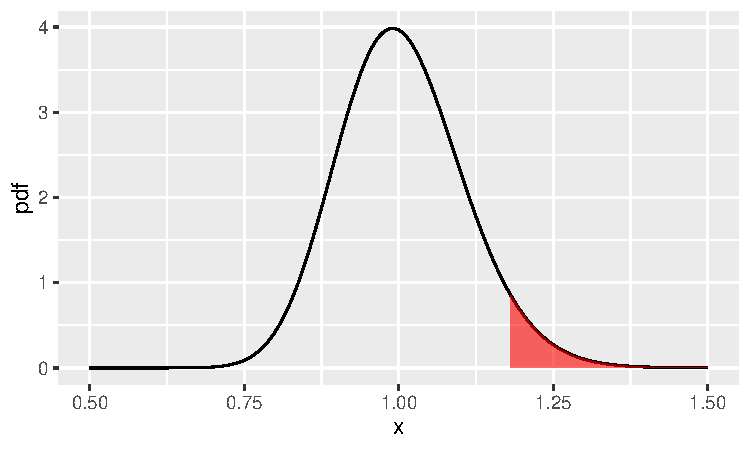
\includegraphics[width = 0.7 \textwidth]{figures/Nanna/Fdistsign.pdf}
  \caption{Pdf for F-distribution with significance level}
  \label{fig:f_dist}
\end{figure}
    
The significance level is illustrated by the area under the curve marked with red, and has area equal to the significance level.
Note that the $pdf$ converges toward a normal distribution, as the degrees of freedom increases.
    
The $F$-statistic is calculated using \eqref{eq:F_statistic}, where the $SSR$ for the two models are calculated by the \texttt{anova} function in R. 
%Kode til Fstat
\begin{lstlisting}
# Residuals
RSS_model1 <- anova(linreg1,linreg0)$RSS[1]; RSS_model1
24.10871
RSS_model0 <- anova(linreg1,linreg0)$RSS[2]; RSS_model0
28.50651
# F-statistic
Fstat <- ((RSS_model0 - RSS_model1)/(dfmod0 - dfmod1))/
((RSS_model1)/(dfmod1)); Fstat
43.67925
\end{lstlisting}
The associated $p$-value is then
\begin{lstlisting}
p <- pf(q = Fstat, df1 = dfmod0, df2 = dfmod1, lower.tail = F)
<2.2e^{-16}
\end{lstlisting}
or effectively zero. We therefore conclude that the additional parameters are statistically significant.
It may seem as though any parameter would be significant, but this is because of our initial filtering and large dataset.
The filtering done in section \ref{sec:modelling} removed parameters with poor fit, thereby only leaving likely significant parameters.
In addition the large dataset also plays a role, since the difference in degrees of freedom is relatively small for many observations. 
This does not mean that the full model is a lot better, since the additional 2 parameters only explain about $9\%$ of the remaining residuals. 

This test was done using only observations from Copenhagen and performing the same procedure for the observations from Aalborg gives $F=0.7301$ and $p=0.5345$.
Meaning that the full model is not significantly better than one containing only $log(size)$ and $year.sale$, when only considering observation from Aalborg.

Alternatively we could check all possible combinations of parameters, to see if any of the the corresponding models contain statistically insignificant parameters.
In order to avoid testing all possible combination it would be beneficial, to determine which parameter adds the least fit to the model and then remove the variables in that order. 

% Choosing the order of which to remove the parameters is known as subset selection and there are several different approaches.
% One method is called backwards step wise selection. 
% The approach is to first remove the parameter that explains the least variation in the data, in order to remove the parameters in a strategic manner.
% More specifically it is a greedy algorithm that starts with the full model, and at each step removes the parameter which adds the least to the $R$-squared.

Backwards selection is used to chose the order of which to remove the parameters.
In table \ref{tbl:backward_order_of_parameters} the order of parameters removal is listed for each of the cities.
    
\begin{table}[H]
    \centering
    \begin{tabular}{r|llll}
        \toprule
        \textbf{Order} & \textbf{Copenhagen} & \textbf{Aarhus} & \textbf{Odense} & \textbf{Aalborg}\\
        \midrule
        1 & $balcony$              & $balcony$         & $cond$            & $cond$ \\
        2 & $cond$           & $cond$            & $balcony$         & $balcony$ \\
        3 & $year.sale$    & $year.sale$  & $year.sale$  & $year.sale$ \\
        4 & $log(size)$         & $log(size)$       & $log(size)$       & $log(size)$ \\
        \bottomrule
    \end{tabular}
    \caption{The order of which backwards stepwise selection removes the parameters for each of the cities.}
    \label{tbl:backward_order_of_parameters}
\end{table}

Using this to compare the full model to one with one removed, we notably get a $p$-value of 0.2944 for Aarhus, 0.3943 for Odense and 0.5025 for Aalborg. 
In the same manner we find the second removed parameter for Aalborg to also be insignificant with a p-value of 0.3678, as expected from the first test.
This means that the following models have significant parameters.
\begin{align*}
    log(price)_{Cph.F} &\sim log(size) + year.sale + cond + balcony \\
    log(price)_{Aar.F} &\sim log(size) + year.sale + cond \\
    log(price)_{Ode.F} &\sim log(size) + year.sale + balcony \\
    log(price)_{Aal.F} &\sim log(size) + year.sale \\
\end{align*}
The F-test only takes the available data into account and can not test how well it aligns with new observations.
It therefore does not measure how good these models are at predicting future apartment prices, and only validates the model based on previouse observations. 



% This means that the model, containing the parameter \textit{selling.period}, is not significantly improved compared to the one without this parameter.
% Comparing the remaining models, we find that all other parameters significantly improves the models. 
% The decision of whether or not to include the additional parameters, then becomes a trade off between better model fit and potential overfitting.
% This will be explored further in the next section.
    
    
    
    % The reason they are still significant is because the decrease in degrees of freedom is relatively small, due to the large set of observations.
    % The $F$-test is therefore best suited for smaller datasets, and we will now look at another way to validate models based on a larger amount of observations. 

\section{Cross-Validation} \label{sec:CV}

Previously we applied the $F$-statistic for the purpose of testing whether or not the model should be restricted. 
As we concluded in section \ref{sec:Ftest}, the $F$-test is more suitable for datasets of fewer observations. 
This is the motivation for using cross validation in order to test the selected variables and the models performance.
Cross-validation is a widely used method for estimating prediction error.
There are many variations of cross-validation, and this project will only cover a limited selection. 

\subsection{\textit{K}-Fold Cross-Validation} 

This method uses part of the data to fit the model and another to test it. This is done via the following process.

The data is split up in $K$ partitions, where one of them is retained as the test or validation fold. 
The remaining $K-1$ partitions are referred to as training sets and are used to fit the model.
This process is repeated $K$ times, where each partition is used as the validation set once. 
This way the entire dataset is used, while keeping the modelling and validation data separate. 

More formally, let $\kappa: \{1, \ldots, n\} \rightarrow \{1, \ldots, K\}$ be the function that indicates which partition observation $i$ belongs to. 
Denote the model fitted with the $k$'th part of the data removed by $(\textbf{x}_i \betahat)^{-\kappa(i)}$. 
Then the cross-validation estimate of the prediction error, for the $k$'th fold, is 
\begin{align*}
    CV(\betahat)_k = \frac{1}{n} \sum_{i=1}^n L\left(y_i, (\textbf{x}_i \betahat)^{-\kappa(i)}\right),
\end{align*}
where we choose the loss function $L\left(y_i, (\textbf{x}_i \betahat)^{-\kappa(i)}\right)=\left(y_i - (\textbf{x}_i \betahat)^{-\kappa(i)}\right)^2$, which indicates how much of the variation in the data is explained by the model fitted from the subset that did not include the $k$'th partition. 

A common choice is $K = 5$, which is what we will use in this project. 
The case $K = n$ is known as leave-one-out cross-validation. 
This tests every possible combination, that is $\kappa(i) = i$. 
This method is approximately unbiased, since each training set is comparatively small, but since the training sets are so similar the variance may be greater. 
Conversely $K=5$ has lower variance, as each training partition is larger, but bias may be a problem. 


\subsection{Application of \textit{K}-fold Cross-Validation}
%Modelselection - forward
In order to test the effect of each parameter, they need to be added one by one. 
% Choosing the order to add the parameters is known as subset selection and there are several different approaches.
We use forward step wise selection to choose the order. The intuition behind this method is:
We want to first add the parameter that individually explains the most variation in the data, in order to end up with the best possible model after having removed some of the parameters.
Here best refers to the model that increases $R$-squared the most.
% More specifically it is a greedy algorithm that starts with the intercept, and at each step adds the parameter with the highest $R$-squared.

After performing the forward stepwise selection on the four cities the order of which the parameters are added can be seen in table \ref{tbl:order_of_parameters}.
To give a little explanation of the table, suppose we want a model considering Aalborg with 2 parameters.
We then choose the Aalborg column and go down to the second row of the table, and see that the model would be on the form $log(price) \sim \log(size) + year.construct$.
\begin{table}[H]
    \centering
    \begin{tabular}{r|llll}
        \toprule
        \textbf{Order} & \textbf{Copenhagen} & \textbf{Aarhus} & \textbf{Odense} & \textbf{Aalborg}\\
        \midrule
        1 & $\log(size)$        & $\log(size)$      & $\log(size)$      & $\log(size)$ \\
        2 & $year.sale$         & $year.sale$       & $year.sale$       & $year.sale$ \\
        3 & $cond$    & $cond$  & $balcony$  & $cond$ \\
        4 & $balcony$           & $balcony$            & $cond$         & $balcony$ \\
        \bottomrule
    \end{tabular}
    \caption{The order of which forward stepwise selection adds the parameters for each of the cities.}
    \label{tbl:order_of_parameters}
\end{table}
%\textbf{TOMMELFINGERREGEL}
%Knowing this, we can make sure that we omit the parameter that contributes least to R-squared first, and thereby achieving the best model. 
%Using this model we now move on to applying cross-validation. 

In figure \ref{fig:CrossValidationCopenhagen} cross-validation is performed for the HOME dataset that only contains the observations for Copenhagen.
For each fold the prediction error (RMSE) has been plotted for each of the six models from table \ref{tbl:order_of_parameters}. Every fold gives varying predictions errors for each model which indicates some randomness crosswise the five folds. The model with the lowest RMSE therefore differs depending on the selected train and testset. 
Thus the interesting result is the meanplot in which the standard errors are calculated for the five folds.
Clearly, the models with most variation crosswise the 5 folds have the highest standard errors. 

To determine the desired number of parameters, the ``one-standard-error'' rule is used. 
This states that we choose the most parsimonious model whose prediction error is no more than one standard error above the prediction error of the best model. The rule is applied to reduce the probability of overfitting and it is therefore expected, that it performs better out-of-sample. Which seems relatively fair, since the increasing in the prediction error is relatively small.

    \begin{figure}[H]
        \centering
      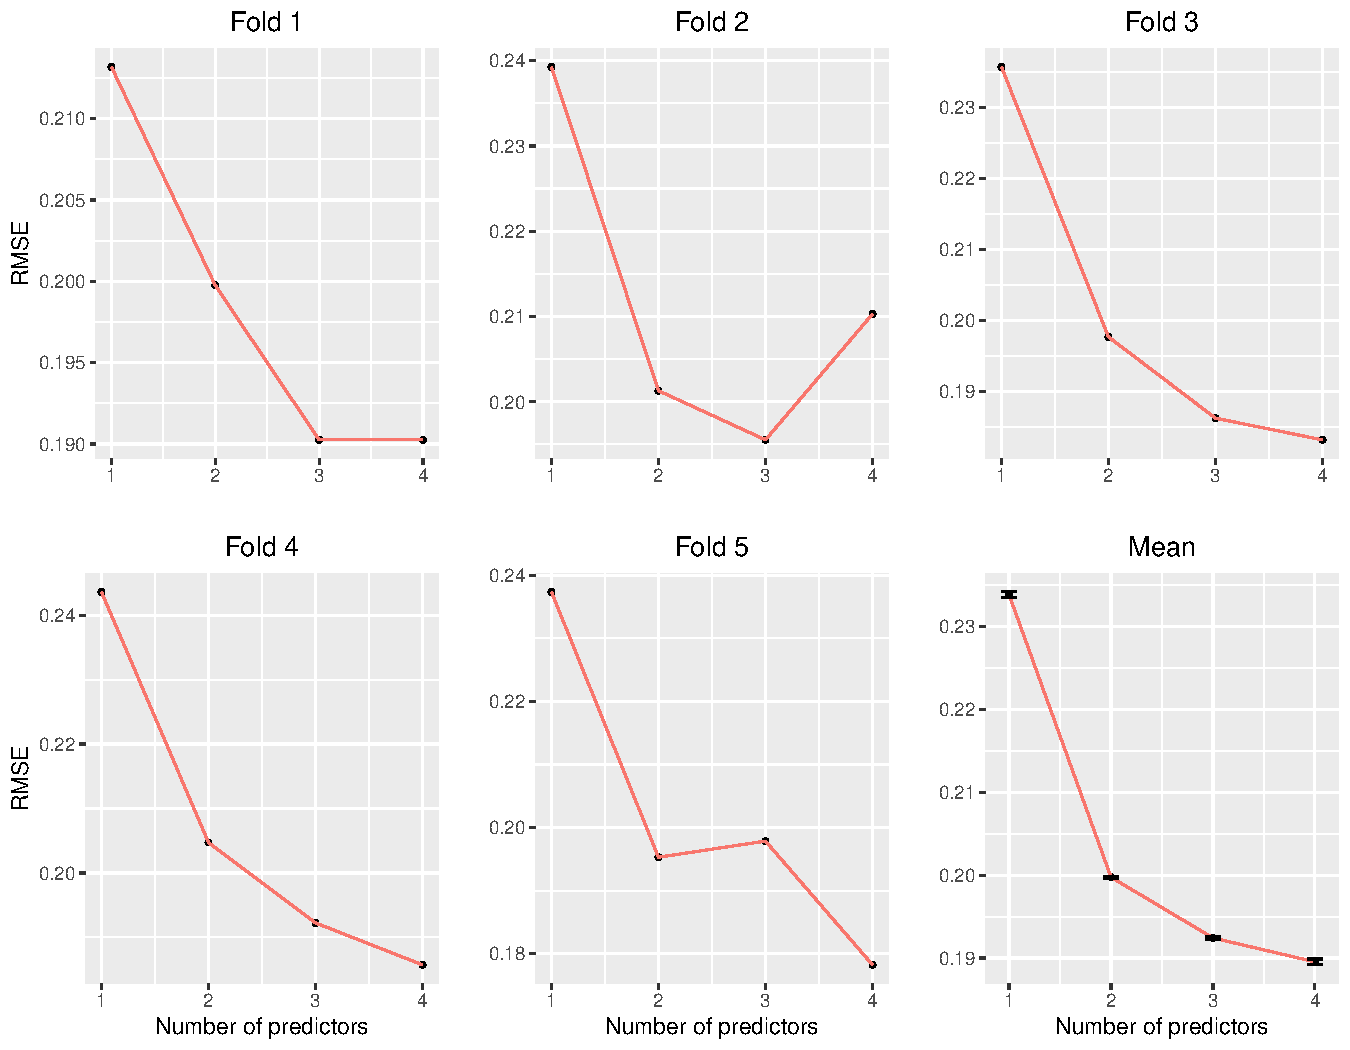
\includegraphics[width = 1 \textwidth]{figures/Nanna/CrossValidationCopenhagen.pdf}
      \caption{Plots of the prediction errors for each fold and their mean with the associated standard errors where the x-axis denotes the number of predictors in the given model.}
      \label{fig:CrossValidationCopenhagen}
    \end{figure}
    
In the case of Copenhagen observe that a model with four parameters has the lowest prediction error, then we choose the smallest number of predictors with a prediction error within the standard error for the model with four parameters.
In this case the optimal number of parameters, according to the rule, is three.

This procedure is performed for the remaining three cities. Note in table \ref{tbl:order_of_parameters} the order of the selected parameters from the execution of the forward-selection-algorithm differs between the cities. 
In figure \ref{fig:CrossValidationSamlet} is the meanplot for each city, in which we conclude from the 5-fold cross-validation, that the optimal number of parameters is three for Aarhus, one for Odense and two forAalborg.

\begin{figure}[H]
    \centering
  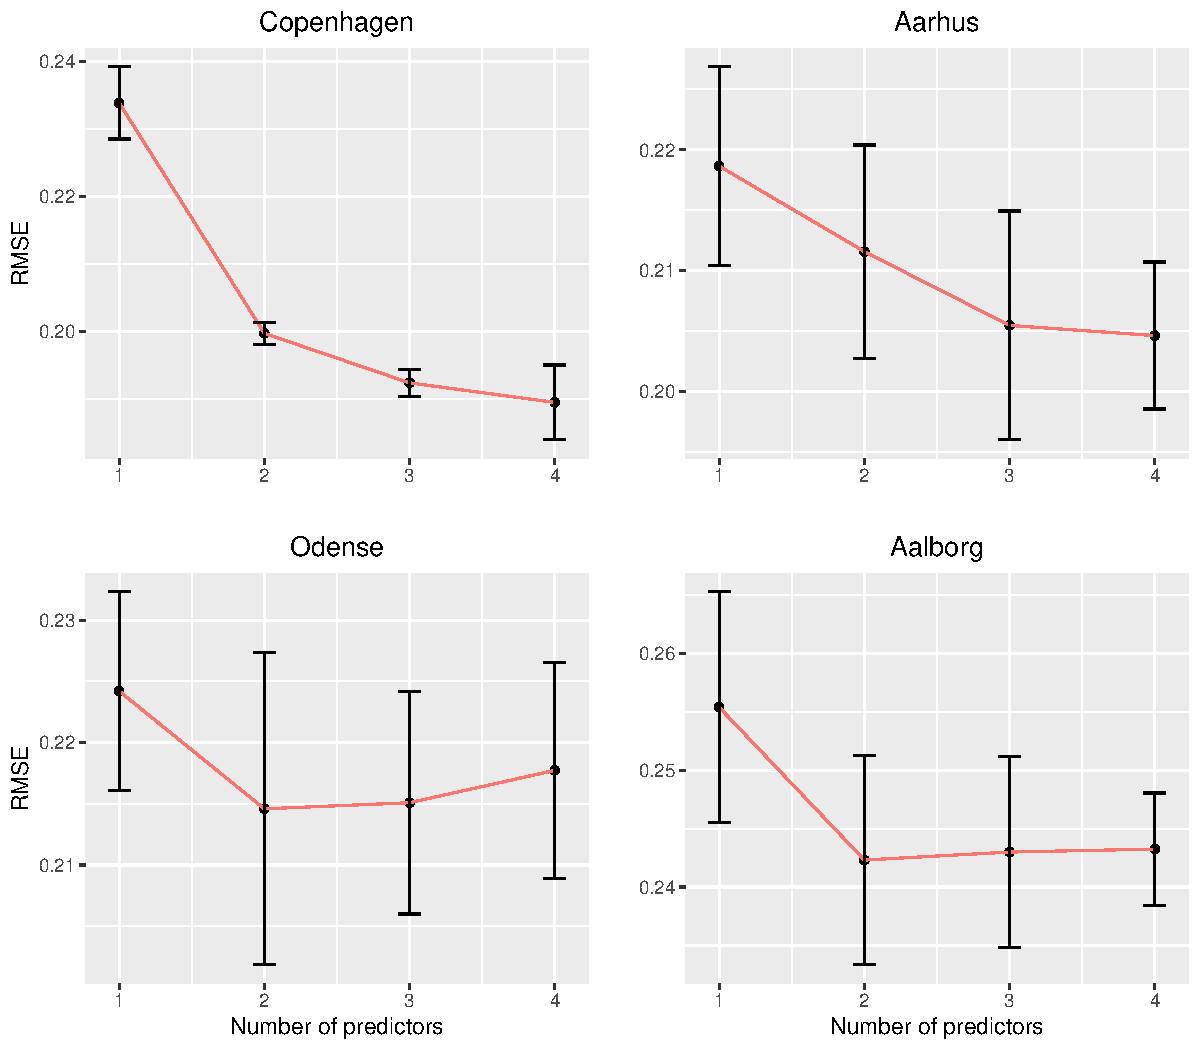
\includegraphics[width = 1 \textwidth]{figures/Nanna/CrossValidationSamlet.pdf}
  \caption{Mean plot for each city with prediction error for each model with associated standard error.}
  \label{fig:CrossValidationSamlet}
\end{figure}

The final models obtained from the result of performing 5-fold cross-validation is listed in appendix \ref{aap:cv} and is listed as follows
\begin{align*}
    log(price)_{Cph.CV} &\sim log(size) + year.sale + cond \\
    log(price)_{Aar.CV} &\sim log(size) + year.sale + cond\\
    log(price)_{Ode.CV} &\sim log(size) \\
    log(price)_{Aal.CV} &\sim log(size) + year.sale \\
\end{align*}
Due to the later purpose of testing the model on out-of-sample performance regarding predicting prices for houses sold in 2016, it is interesting to investigate the out-of-sample performance on the selected models from CV.
If the errors fulfil the earlier stated assumptions regarding normally distributed errors with mean zero and \homo, when we expect the model to perform well out-of-sample. In figure \ref{fig:cv_normal_homo} the errors obtained from the CV of Copenhagen are presented.

\begin{figure}[H]
\centering
\begin{subfigure}[b]{0.5\textwidth}
    \centering
    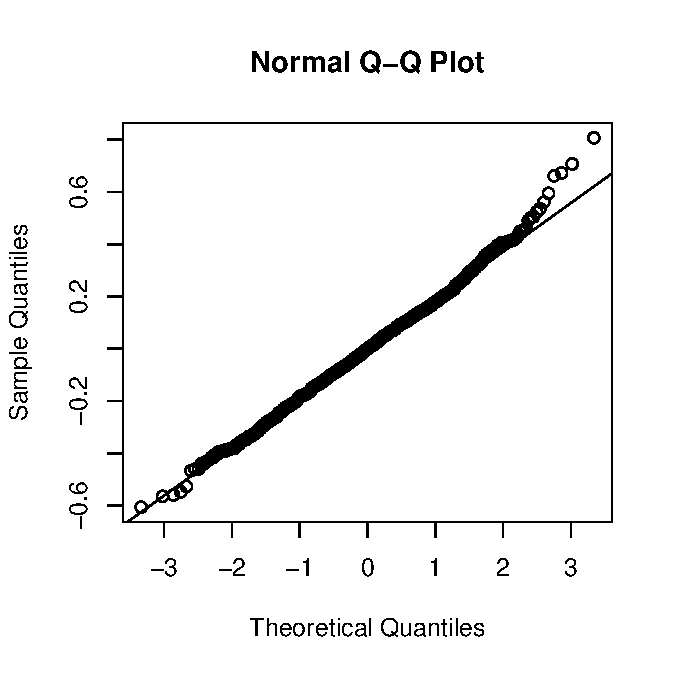
\includegraphics[width = \textwidth]{figures/Nanna/Normal.pdf}
    \caption{Testing for normality}
    \label{fig:cv_normal}
\end{subfigure}%
\begin{subfigure}[b]{0.5\textwidth}
\centering
    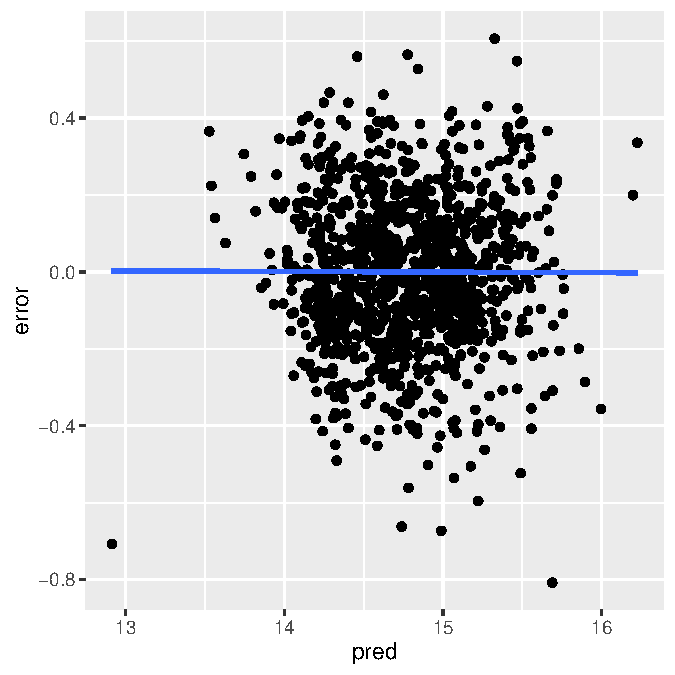
\includegraphics[width = \textwidth]{figures/Nanna/cv_normal_homo.pdf}
    \caption{Testing for \hetero}
    \label{fig:cv_homo}
\end{subfigure}
\caption{Examination of the prediction errors from the 5-fold cross validation.}
\label{fig:cv_normal_homo}
\end{figure}

From figure \ref{fig:cv_normal} it is concluded that there are problems in the tails of the errors. 
In the tails there are deviations from what is expected of the normal distribution. 
This might cause problems with both the confidence and prediction interval of the model, since this does not take the larger tails into account.
The tails indicates, that the intervals should be enlarged.
Therefore, the model is now suspected to have some difficulties performing out-of-sample. 
In figure \ref{fig:cv_homo} the errors seems overall homoskedastic with mean zero. 

\section{Residuals}\label{subsec:residuals}
So far we have only discussed residuals in passing. 
This chapter will therefore present different types of residuals and their properties.
Residuals are the difference between the observed values $\textbf{y}$ and the fitted values $\hat{\textbf{y}}$. They are therefore the errors $\boldsymbol{\hat{\varepsilon}}$ described in \eqref{eq:replace_with_y}
\begin{align*}
    \textbf{r}(\textbf{y}) &= \textbf{y} - \hat{\textbf{y}} = \textbf{y} - \textbf{X} \betahat = (\textbf{I} - \textbf{H}) \textbf{y}.
    % r_i(y) &= y_i - x_i \betahat = y_i - x_i (X^\top X)^{-1}X^\top y_i = (1 - h_{ii}) y_i,
\end{align*}
By assumption \ref{as:normality_of_errors} the residuals have variance
\begin{align*}
    Var(\textbf{r}(\textbf{Y})) &= \sigma^2 (\textbf{I} - \textbf{H}) \\
    Var(r_i(\textbf{Y})) &= \sigma^2(1 - h_{ii}),
\end{align*}
where $h_{ii}$ is the $i$'th diagonal element in $\textbf{H}$. The second equation follows, since the first equation is just the variance-covariance matrix for the residuals, which has variances in the diagonal.
Rewriting \eqref{eq:unbiased_variance_estimate} using projection matrices gives the following estimate for the parameter variance
\begin{align*}
    s^2(\textbf{Y}) &= \frac{\| \textbf{Y} - \textbf{X} \betahat (\textbf{y}) \|^2 }{n-k-1} = \frac{\| \textbf{Y} - \textbf{H} \textbf{Y} \|^2}{n-k-1} .
\end{align*}
Residuals can be used to identify outliers, which is the observations that do not fit the general pattern of the data.
These data points can have a large effect on the estimated variance and it would therefore be useful to have a way to measure how much variance an observation adds.
We use the notation $-i$, which refers to the removal of the $i$'th row e.g.
\begin{align*}
    \textbf{y}_{-i} = (y_1, \ldots, y_{i-1}, y_{i+1}, \ldots, y_n)^\top.
\end{align*}
The estimate for $\sigma^2$ found by deleting the $i$'th row is then
\begin{align*}
    \hat{\sigma}^2_{-i}(\textbf{Y}) = \frac{\| \textbf{Y}_{-i} - \textbf{H}_{-i} \textbf{Y}_{-i} \|^2}{n-1-(k+1)}.
\end{align*}
We now introduce the studentized residual $(\textbf{r}^{rt})$, which takes into account the variance without the i'th observation, thereby giving a more accurate measure of the standard deviation
\begin{align*}
    r_i^{rt} = \frac{r_i}{\sqrt{\hat{\sigma}^2_{-i}(1-h_{ii})}}.
\end{align*}
If this value in deemed to high, it should be investigated and could potentially justify removing it as an outlier/measurement error. We now introduce an important property of the studentized residuals.

\begin{proposition}
    Consider a general linear model $\textbf{Y} \sim N_n(\textbf{X} \betabold, \sigma^2 \textbf{I}_n)$ where the design matrix has full rank $k \leq n-3$ and $\textbf{H} = \textbf{X} (\textbf{X}^\top \textbf{X})^{-1}\textbf{X}^\top$ is the corresponding projection-matrix, then
    \begin{align*}
        r_i^{rt}(\textbf{Y}) \sim t(n-k-2).
    \end{align*}
\end{proposition}
\begin{proof}
    Without loss of generality let $i=1$. 
    To summarize the above results
    \begin{align*}
        r_1^{rt}(\textbf{Y}) = \frac{r_1(\textbf{Y})}{\sqrt{\hat{\sigma}^2_{-1}(\textbf{Y}_{-1})(1-h_{11})}}
        =
        \frac{r_1(\textbf{Y})/ \sqrt{\sigma^2 (1-h_{11})}}{\sqrt{\hat{\sigma}_{-i}^2 (\textbf{Y}_{-1})/\sigma^2}},
    \end{align*}
    which has the distribution
    \begin{align*}
        \frac{N(0,1)}{\sqrt{\chi^2(n-k-2)/(n-k-2)}} = t(n-k-2)
    \end{align*}
    Therefore we just need to prove that they are independent.
    Using the definition of the residual $r_1(\textbf{Y}) = Y_1 -  (\textbf{HY})_1$ and the projection matrix
    \begin{align*}
        \begin{bmatrix}
            r_1(\textbf{Y}) \\
            \textbf{Y}_{-1} - \textbf{H}_{-1} \textbf{Y}_{-1}
        \end{bmatrix}
        =
        \begin{bmatrix}
            Y_1 - \textbf{x}_1^\top (\textbf{X}^\top \textbf{X})^{-1} \textbf{X}^\top \textbf{Y} \\
            \textbf{Y}_{-1} - \textbf{X}_{-1} (\textbf{X}_{-1}^\top \textbf{X}_{-1})^{-1} \textbf{X}_{-1}^\top \textbf{Y}_{-1}
        \end{bmatrix}
    \end{align*}
    This can be written as the matrix-vector product
    \begin{align*}
        \begin{bmatrix}
            1 - \textbf{x}_1^\top (\textbf{X}^\top \textbf{X})^{-1} \textbf{x}_1^\top & - \textbf{x}_1^\top (\textbf{X}^\top \textbf{X})^{-1} \textbf{X}_{-1}^\top \\
            \textbf{0} & \textbf{I}_{n-1} - \textbf{X}_{-1} (\textbf{X}_{-1}^\top \textbf{X}_{-1})^{-1} \textbf{X}_{-1}^\top
        \end{bmatrix}
        \begin{bmatrix}
            Y_1 \\
            \textbf{Y}_{-1}
        \end{bmatrix}
        =
        \textbf{AY} =
                \begin{bmatrix}
            \textbf{A}_1 \\
            \textbf{A}_2
        \end{bmatrix}
        \textbf{Y}
        \sim N(\cdot)
              \
    \end{align*}
    Therefore $\textbf{A}_1 \textbf{Y} = r_1(\textbf{Y})$ and $\textbf{A}_2 \textbf{Y} = \textbf{Y}_{-1} - \textbf{H}_{-1} \textbf{Y}_{-1}$ are independent if they are uncorrelated. Their covariance matrix is given by 
    \begin{align*}
        \cov(\textbf{A}_1 \textbf{Y}, \mathbf{A}_2 \textbf{Y}) &= \textbf{A}_1\  \var(\textbf{Y}) \ \textbf{A}_2^\top = \textbf{A}_1 \sigma^2 \textbf{I}_n \textbf{A}_2^\top = \sigma^2 \textbf{A}_1 \mathbf{A}_2^\top \\
        &= \sigma^2 
        \begin{bmatrix}
            1 - \textbf{x}_1^\top (\textbf{X}^\top \textbf{X})^{-1} \textbf{x}_1^\top & - \textbf{x}_1^\top (\textbf{X}^\top \textbf{X})^{-1} \textbf{X}_{-1}^\top
        \end{bmatrix}
        \cdot
        \begin{bmatrix}
            \textbf{0}^\top \\
            \textbf{I}_{n-1} - \textbf{X}_{-1} (\textbf{X}_{-1}^\top \textbf{X}_{-1})^{-1} \textbf{X}_{-1}^\top
        \end{bmatrix} \\
        &= \sigma^2 (- \textbf{x}_1^\top (\textbf{X}^\top \textbf{X})^{-1} \textbf{X}_{-1}^\top) (\textbf{I}_{n-1} - \textbf{X}_{-1} (\textbf{X}_{-1}^\top \textbf{X}_{-1})^{-1} \textbf{X}_{-1}^\top) \\
        &= \sigma^2 (- \textbf{x}_1^\top (\textbf{X}^\top \textbf{X})^{-1} \textbf{X}_{-1}^\top + \textbf{x}_1^\top (\textbf{X}^\top \textbf{X})^{-1} \textbf{X}_{-1}^\top \textbf{X}_{-1} (\textbf{X}_{-1}^\top \textbf{X}_{-1})^{-1} \textbf{X}_{-1}^\top) \\
        &= \sigma^2 (- \textbf{x}_1^\top (\textbf{X}^\top \textbf{X})^{-1} \textbf{X}_{-1}^\top + \textbf{x}_1^\top (\textbf{X}^\top \textbf{X})^{-1} \textbf{X}_{-1}^\top) \\
        &= \textbf{0},
    \end{align*}
    and therefore uncorrelated and because they are jointly normally distributed also independent.
\end{proof}

The distribution of the studentized residuals should therefore be checked, in order to verify assumption \ref{as:normality_of_errors}. 
Since the $t$-distribution converges toward the normal distribution for large datasets, a plot similar to \ref{fig:studentized_res_plot} is often made.

\subsection{Application of Studentized Residuals} \label{sub:residuals}

In this application we want to verify the earlier stated assumption \ref{as:normality_of_errors} about the errors of the models obtained from the $F$-test and from the 5-fold cross-validation. 
Since the error term is unobserved, the investigation is performed on the residuals of the models.
Copenhagen is the illustrated case in figure \ref{fig:studentized_res_plot}, but Aarhus and Odense also have different results from the $F$-test compared to cross-validation.

Both models seem to comply well with assumption \ref{as:normality_of_errors}, and are almost exactly the same.
Both have more data located at the left tail of the distribution, as compared to the normal distribution. 
This means there are more large negative errors than expected, which is obviously undesirable for a model used for prediction. 
This is only a problem for a small part of the dataset, and the model may therefore still be good as a rough estimate. 
As a result, we expect that the 95\% prediction interval and the 95\% confidence interval of the models should be larger, given that these are calculated for the normal distribution.

\begin{figure}[H]
    \centering
  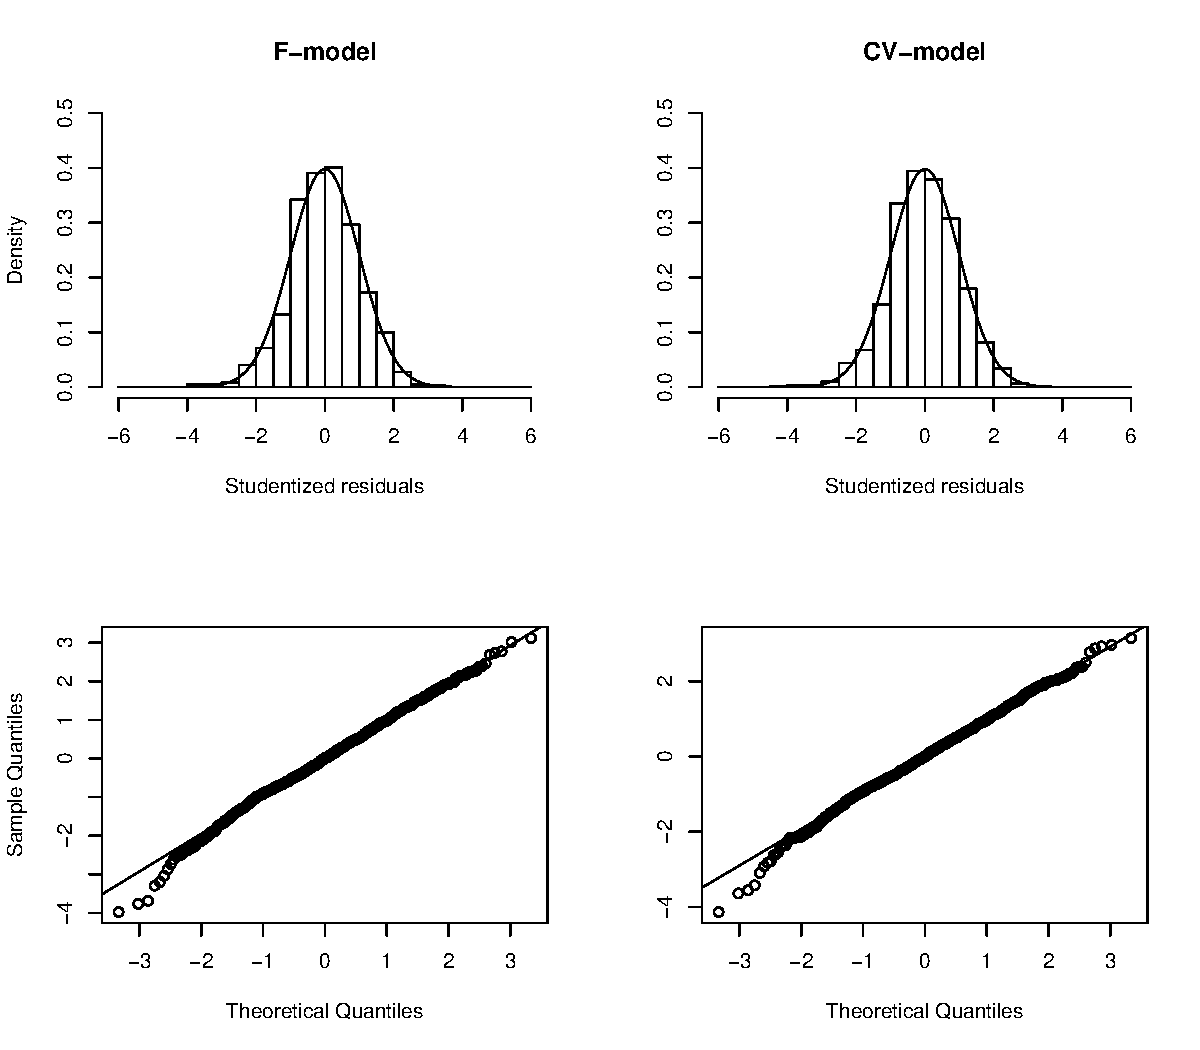
\includegraphics[width = 0.9 \textwidth]{figures/Nanna/studentized_res_plot.pdf}
  \caption{QQ-plot and histogram plot for the studentized residuals for the F-model and CV-model respectively for Copenhagen.}
  \label{fig:studentized_res_plot}
\end{figure}

For Odense the residuals are approximately normal distributed and there is no noteworthy difference in the residuals of the two models.
This is a general result for the remaining cities as the residuals is almost the same for the models from $F$-test compared to those found by cross-validation and they are approximately normal distributed.
However, the residuals of the models for Aarhus and Aalborg differ the most from a normal distribution, as illustrated for Aalborg in figure \ref{fig:studentized_res_plot_Aalborg}.
Therefore, we expect the Aalborg model to have slightly inferior predictive performance compared to the other models.

\begin{figure}[H]
    \centering
  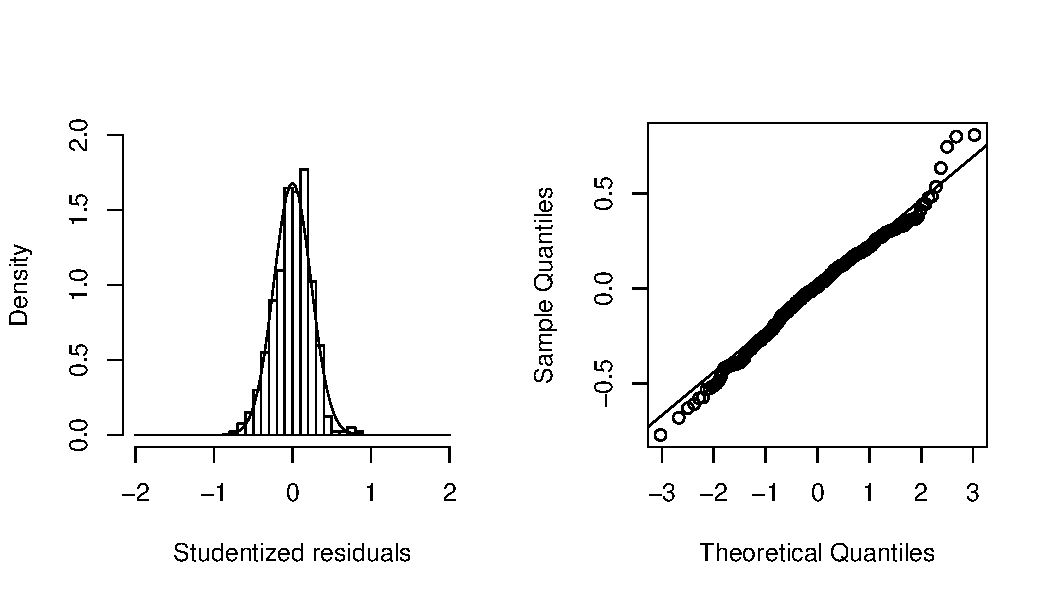
\includegraphics[width = 0.95 \textwidth]{figures/Nanna/NormalAal.pdf}
  \caption{QQ-plot and histogram plot for the studentized residuals of the models for Aalborg.}
  \label{fig:studentized_res_plot_Aalborg}
\end{figure}

% The same data as in section ?? is used
% \begin{lstlisting}
%     #The studentized residuals are found for each model
%     res1 <- rstudent(mod1)
%     res2 <- rstudent(mod2)
    
%     #Histogram for the residuals, and associated normal distribution
%     hist(res1,prob=TRUE); curve(dnorm(x,mean(res1),sd(res1)),add=TRUE)
%     hist(res2,prob=TRUE); curve(dnorm(x,mean(res2),sd(res2)),add=TRUE)
% \end{lstlisting}
% The residuals for both models clearly follow a normal distribution and assumption \ref{as:normality_of_errors} is therefore satisfied, as illustrated in figure \ref{fig:studentized_res_plot}.
%     \begin{figure}[H]
%         \centering
%       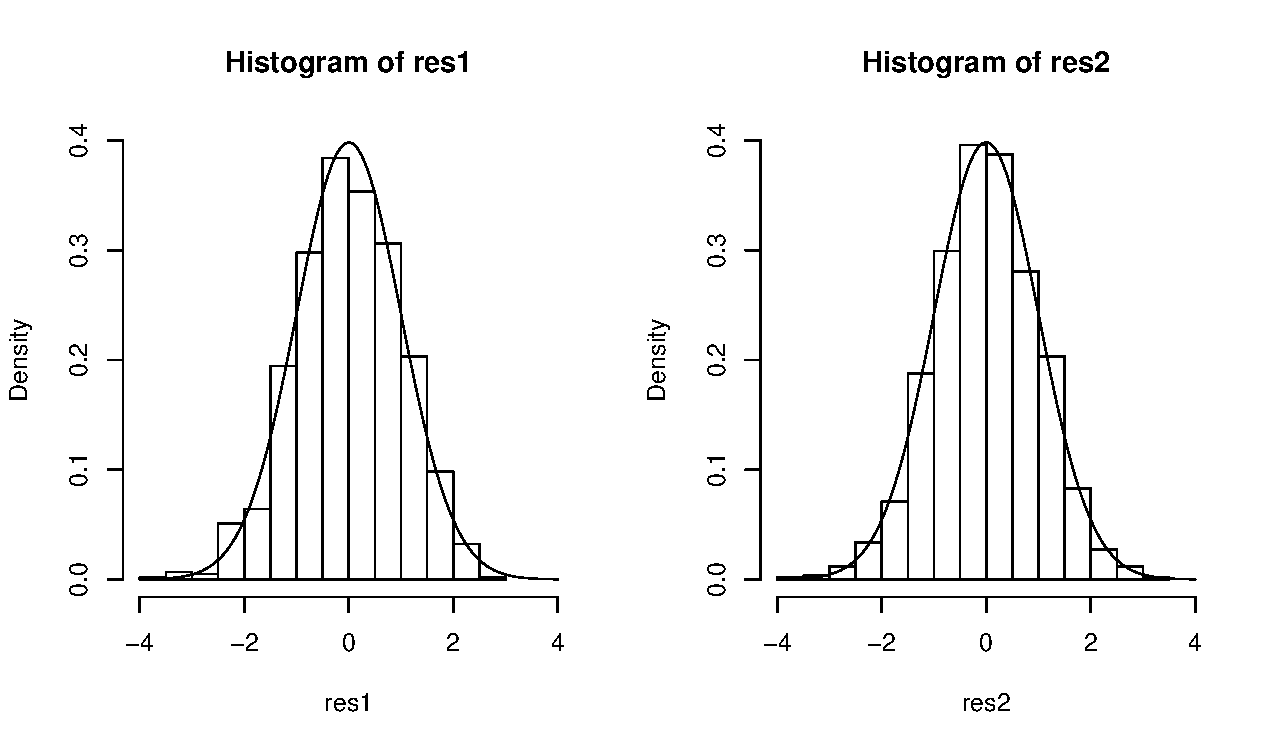
\includegraphics[width = 1 \textwidth]{RRESIUDALPLOT_HISTOGRAM.pdf}
%       \caption{Distribution of Studentized Residuals.}
%       \label{fig:studentized_res_plot}
%     \end{figure}


\section{Testing and Correcting for Heteroskedasticity}
In this section we wish to introduce methods for detecting heteroskedasticity and afterwards how to correct for heteroskedasticity so it is possible to test hypotheses when evaluating our models in the case of heteroskedasticity.

\subsection{Test for Heteroskedasticity}
In this section we wish to introduce a method to determine if heteroskedasticity is present, because in the case of heteroskedasticity the usual OLS estimator is not BLUE c.f.$\!$ \ref{as:homoskedasticity_and_no_serial_correlation}. 

We consider our linear model given as $\textbf{y} = \textbf{X} \betabold + \boldsymbol{\varepsilon}$ and let assumption \ref{as:linear_in_the_parameters}, \ref{as:no_perfect_collinearity} and \ref{as:zero_conditional_mean} hold. We then construct our null hypothesis as
\begin{align*}
    \mathcal{H}_0 : \var[\boldsymbol{\varepsilon} | \mathbf{X}] = \var[\boldsymbol{\varepsilon}] = \sigma^2 \textbf{I}_n. 
\end{align*}
With this null hypothesis we wish to determine if the homoskedasticity assumption holds true. 
If we accept our $\mathcal{H}_0$-hypothesis for a small significance level, then heteroskedasticity is with a high probability not present.
Assumption \ref{as:zero_conditional_mean}, which says that the conditional expected value of $\boldsymbol{\varepsilon}$ is equal to $\textbf{0}$, implies that $\var(\boldsymbol{\varepsilon} | \mathbf{X}) = E[\boldsymbol{\varepsilon \varepsilon^\top} | \mathbf{X}]$ because of the conditional variance formula $\var(\boldsymbol{\varepsilon} | \mathbf{X}) = E[\boldsymbol{\varepsilon \varepsilon^\top} | \mathbf{X}] - E[\boldsymbol{\varepsilon} | \mathbf{X}]E[\boldsymbol{\varepsilon}^\top | \mathbf{X}]$. 
Using this we rewrite our $\mathcal{H}_0$-hypothesis as
\begin{align*}
    \mathcal{H}_0 : E[\boldsymbol{\varepsilon \varepsilon^\top} | \mathbf{X}] = E[\boldsymbol{\varepsilon \varepsilon^\top}] = \sigma^2\textbf{I}_n.
\end{align*}
With this $\mathcal{H}_0$-hypothesis we test if the error term, $\sigma^2$ is related with any of the explanatory variables in terms of the expected value.  
If $\mathcal{H}_0$ is rejected then $\sigma^2_i$ is a function of at least one of the explanatory variables, so the error term can be expressed as a linear function of these explanatory variables
\begin{align}\label{eq:test_hetero_nul_hypotese}
    \sigma_i^2 = \delta_0 + \delta_1x_{i,1} + \ldots + \delta_kx_{i,k} + v_i
\end{align}
where $v_i$ is an error with mean equal to $0$ given the explanatory variables. In order for $\sigma_i^2$ to be homoskedastic the following $\mathcal{H}_0$-hypothesis must be accepted 
\begin{align}\label{eq:H_nul_for_hetero_med_delta}
    \mathcal{H}_0 : \delta_1 = \delta_2 = \ldots = \delta_k = 0.
\end{align}
So the error term $\textbf{v}$ does not depend on the explanatory variables. 
If the error $v_i$ is assumed to be independent of the explanatory variables $\mathbf{X}$, then the $F$-statistics can be used to test \eqref{eq:H_nul_for_hetero_med_delta} for the overall significance of the explanatory variables for $\sigma^2$, even though this error term is not normally distributed. This is shown by the Central Limit Theorem, which we state without proof. 
\begin{theorem}[Central Limit Theorem] \label{th:Central_limit_theorem}
Let $S_n = \{ Y_1, Y_2, \ldots, Y_n \}$ be an i.i.d.$\!$ random sample with mean $\mu$ and variance $\sigma^2 < \infty$. Then
\begin{align} \label{eq:bakergud}
    P\left(\dfrac{S_n - n\mu}{\sigma \sqrt{n}}\leq y\right) \rightarrow \Phi(y)
\end{align}
where $\Phi(y)$ is the cdf of the standard normal distribution and $S_n$ is the sum of $Y$. 
\end{theorem}
From the central limit theorem it is possible to derive the distribution of $S_n$. 
We have equation \eqref{eq:bakergud} and for large $n$ we use the central limit theorem to rewrite as
\begin{align*}
    Z_n = \dfrac{S_n - n\mu}{\sigma \sqrt{n}} \stackrel{d}{\sim} N(0,1). 
\end{align*}
Where $\stackrel{d}{\sim}$ denotes the approximate distribution. It is seen that $S_n$ has mean $n\mu$ and variance $n \sigma^2$ from the above equation. We use this to write
\begin{align*}
    S_n \stackrel{d}{\sim} N(n\mu, n\sigma^2). 
\end{align*}
This means that the sum of i.i.d. random variables $S_n$ have an approximately normal distribution regardless of how $Y$ is distributed. Therefore an $F$-test for $\sigma_i^2$ is asymptotically true even though $\sigma_i^2$ is not normally distributed.  




Since $\sigma^2_i$ is unobserved we cannot calculate the OLS regression on $\sigma_i^2$ for $\mathbf{X}$, so instead we calculate the regressions using the estimates. Thus
% \begin{align}\label{eq:OLS_residual_hat_epsioln_i_anden}
%     \hat{\boldsymbol{\varepsilon}}\hat{\boldsymbol{\varepsilon}}^\top = \delta_0\textbf{1} + \delta_1\textbf{x}_1 + \ldots + \delta_k\textbf{x}_k + \mathbf{w}
% \end{align}
\begin{align}\label{eq:OLS_residual_hat_epsioln_i_anden}
    s_i^2 = \delta_0 + \delta_1x_{i,1} + \ldots + \delta_kx_{i,k} + w_i,
\end{align}
where $s^2_i$ is an estimate for $\sigma^2_i$ and $w_i$ has mean 0. From this equation the $F$-statistics for the joint significance of $\textbf{x}_1, \textbf{x}_2, \ldots, \textbf{x}_k$ can be calculated to test for multicollinearity.

In addition to section \ref{sec:Ftest} the $F$-statistic can be used to test for the overall significance of a regression. 
Consider the model with $k$ independent variables, to which the null hypothesis can be written as
\begin{align}\label{eq:null_hypo_for_F_overall_significance_R}
    \mathcal{H}_0: \beta_1 = \beta_2 = \ldots = \beta_k = 0.
\end{align}
Where the alternative hypothesis is that at least one estimator is non-zero. In \eqref{eq:null_hypo_for_F_overall_significance_R} there are $k$ restrictions and they state that knowing the values of the explanatory variables does not explain the dependent variable $y$. This can be written as
\begin{align}\label{eq:unrestricted_F_hypo_for_jeg_skal_bruge_den}
    y_i = \beta_0 + \varepsilon_i.
\end{align}
Where all independent variables have been excluded due to no effect on $y$. 
Recall equation \eqref{eq:F_test_R}, which is the $F$-statistics using the $R$-squared. 
In the restricted model \eqref{eq:unrestricted_F_hypo_for_jeg_skal_bruge_den} the $R$-squared is equal to $0$ because none of the variation in $y$ is accounted for because there are no explanatory variables. 
Furthermore $q = df_0 - df_{1}$ is equal to $k$ because $df_0 = n-0-1$ and $df_{1} = n-k-1$ which means $q = n-1 - (n-k-1) = k$. 
If we substitute this into \eqref{eq:F_test_R} we get
\begin{align}\label{eq:udvidelse_til_F_stat}
    F = \dfrac{R^2_{s_i^2}/k}{(1-R^2_{s_i^2}) / (n-k-1)}
\end{align}
Here $R^2_{s_i^2}$ is the $R$-squared found from \eqref{eq:OLS_residual_hat_epsioln_i_anden} and $k$ is the number of independent variables in \eqref{eq:OLS_residual_hat_epsioln_i_anden}.
This $F$-statistics in only valid in testing for joint exclusion of all independent variables. 
Therefore it often referred to as the overall significance of the regression. 

We summarise the steps in this procedure as follows

\textbf{Test for Heteroskedasticity}
\begin{enumerate}[label=(\roman*)]
    \item Estimate the linear regression model \eqref{eq:multiple_linear_regression_model} by OLS and obtain the squared OLS residuals $s_i^2$. 
    \item Make the regression on \eqref{eq:OLS_residual_hat_epsioln_i_anden} and calculate the $R^2_{s_i^2}$. 
    \item Perform the $F$-statistics. If the $p$-value is below the significance level, reject the null hypothesis. 
\end{enumerate}

This means that if the $p$-value if sufficiently small for the $F$-statistic, then heteroskedasticity is present. 

% \begin{example}[Test for Heteroskedasticity]

% Først laver vi vores test for homoskedasticitet vha. teorien fra project (Breusch-Pegan Test): 


% $Storbyer2 <- na.omit(Storbyer)
% lin.model <- lm(Kontantpris ~ Boligtilstand + Boligareal + Liggetid + Opfoerelsesaar + Altan + OmbygningSket + By, data = Storbyer2); lin.model
% summary(lin.model)$

% $resi <- residuals(lin.model); resi$


% $var_lin.model <- lm(resi^2 ~ Boligtilstand + Boligareal + Liggetid + Opfoerelsesaar + Altan + OmbygningSket + By, data = Storbyer2); var_lin.model
% summary(var_lin.model)$


% Vi sammenligner med R's indbyggede test (Breusch-Pegan Test)

% bptest(lin.model)


% Vi ser at vi får samme p-værdi ved begge test. Da denne p-værdi er mindre end 0.05 forkaster vi nulhypotesen som er at der findes homoskedasticitet i dataet. Dvs. at der heteroskedasticitet tilstede i dataet. 

% I forbindelse med at kunne bruge vores OLS vil vi lave roboste standard errors som så kan bruges til at lave robuste t/- og F teste med således vi stadig kan bruge og vurdere OLS. 

% \end{example}

\subsection{Correct for Heteroskedasticity}
To sum up, \hetero will in general cause OLS standard errors to be faulty as well as the related statistical tests. In this section we wish to correct for these mistakes, so the related statistical tests are valid when testing our hypotheses. 

If our model contains heteroskedasticity, then the errors will not be constant. Thus for our model, $y_i = \textbf{x}_i\betabold + \varepsilon_i$, the variance of the error term is given as
\begin{align*}
    \var(\varepsilon_i | \mathbf{x}_i) = \sigma^2_i. 
\end{align*}
Where the subscript $i$ indicates that the error term varies with the explanatory variables. 

In order to find standard errors which are applicable in $t$-tests when heteroskedasticity is present, we must have a valid expression for $\var(\betahat|\textbf{X})$, which is found using \eqref{eq:conditional_variance_of_epsilon}. 
\begin{align*}
   \var(\betahat|\mathbf{X}) &= (\mathbf{X}^\top\mathbf{X})^{-1}\mathbf{X}^\top\left[ \var(\boldsymbol{\varepsilon} | \mathbf{X}) \right] \mathbf{X}(\mathbf{X}^\top\mathbf{X})^{-1}\\
   &= (\mathbf{X}^\top \mathbf{X})^{-1}\mathbf{X}^\top \sigma^2 \Sigma \mathbf{X}(\mathbf{X}^\top \mathbf{X})^{-1}\\
   &= \sigma^2 (\mathbf{X}^\top \mathbf{X})^{-1}\mathbf{X}^\top \Sigma \mathbf{X} (\mathbf{X}^\top \mathbf{X})^{-1}
\end{align*}
Where $\Sigma$ is a covariance matrix different from the identity matrix so $\var(\boldsymbol{\varepsilon}|\textbf{X}) = \sigma^2 \Sigma$. It can be shown that a valid estimator of $\var(\betahat|\textbf{X})$ is
\begin{align}\label{eq:estimat_varians_beta_hetero}
    \widehat{\var(\betahat)} = \dfrac{\nsum \hat{r}^2_{ij} \hat{\boldsymbol{\varepsilon}}\hat{\boldsymbol{\varepsilon}}^\top}{SSR_j^2}. 
\end{align}
Where $\hat{r}^2_{ij}$ is the $i$'th residual found by regressing $x_j$ on all other independent variables and $SSR_j$ is found by regressing $x_j$ on all other independent variables. 
The standard errors of $\betahat$ are then obtained by taking the square root of \eqref{eq:estimat_varians_beta_hetero} and we call these standard errors \textbf{heteroskedastic robust standard errors}. 

When the heteroskedastic robust standard errors are found it is possible to construct valid $t$-tests in the presence of heteroskedasticity. 
Recall the general $t$-test in \eqref{eq:t_test1}. When heteroskedasticity is present a valid $t$-statistics is obtained using the square root of \eqref{eq:estimat_varians_beta_hetero} as the standard error. 

A heteroskedastic robust $F$-statistic is also called a heteroskedastic Wald-Statistic. In the $F$-statistics we wish to test if the regressions coefficients can be written as a linear combination to see if our restrictions hold true. Our null-hypothesis is
\begin{align*}
    \mathrm{H}_0 : \mathbf{R}\betabold = \mathbf{r}. 
\end{align*}
Where $\mathbf{r}$ is a $q \times 1$ vector, $\betabold$ is a $(k+1) \times 1$ vector and $\mathbf{R}$ is a $q \times (k+1)$ matrix which has full row rank, $rank(\mathbf{R}) = q$ and therefore $q < k+1$. The representation of $\mathbf{R}$ is determined by the hypothesis wished to be examined. 

For an example consider the general linear model $y_i = \beta_0 + x_{i,1}\beta_{1} + x_{i,2}\beta_{2} + x_{i,3}\beta_{3} + \varepsilon_i$. We wish to test if $\beta_2 = \beta_3$ and if $\beta_3 = 0$. These two equations are the hypothesis and thus $q = 2$. We represent this in matrix form as
\begin{align*}
    \mathbf{R} = \begin{bmatrix}0 & 1 & -1 & 0\\
    0 & 0 & 0 & 1\end{bmatrix}, \mathbf{r} = \begin{bmatrix}0\\0\end{bmatrix}.
\end{align*}

The $F$-statistics is defined as
\begin{align*}
    F &\equiv \dfrac{(\mathbf{R}\betahat - \mathbf{r})^\top  [\mathbf{R}(\mathbf{X}^\top \mathbf{X})^{-1}\mathbf{R}^\top]^{-1}  (\mathbf{R}\betahat- \mathbf{r}) / q}{s^2} \sim F_{q, n - (k+1)}\\
\end{align*}
% However if the errors have differing variance then this F-statistic will fail to be valid.  Recall that in the presence of heteroskedasticity OLS estimators, $\betahat$, will still be unbiased and consistent however they will fail to be efficient and the standard errors estimated with OLS will prove to be faulty to which they cannot be used in hypotheses testing because they are biased and inconsistent. 
% Instead the heteroskedastic-robust Wald Statistic is used, where the Wald statistic is given as
% \begin{align*}
%     W = (\mathbf{R}\betahat - \mathbf{r})^\top (\mathbf{R} \widehat{\var(\betahat|\mathbf{X}})(\mathbf{R}\betahat - \mathbf{r}))
% \end{align*}
% This statistic is approximately $\chi^2_q$-distributed. If it is divided by $q$ it becomes an approximate $F$-statistic with $(q,q-k-1)$ degrees of freedom. Thus
% \begin{align*}
%     F = (\mathbf{R}\betahat - \mathbf{r})^\top (\mathbf{R} \widehat{\var(\betahat|\mathbf{X}})(\mathbf{R}\betahat - \mathbf{r}))/q
% \end{align*}
In the case of heteroskedasticity these tests are preferable. 
The $t$-test also work in the case of homoskedasticity, but the usual OLS standard errors are still preferable because in the case of homoskedasticity $t$-tests will have exact $t$-distributions. 

We have conducted tests for heteroskedasticity for the models chosen in sections regarding $F$-tests and cross-validation.
We present the result for the model chosen for Copenhagen via $F$-tests. 

The model for Copenhagen determined by the $F$-test is
\begin{align}
    log(price) \sim log(size) + cond + balcony + year.sale
\end{align}
We tested for heteroskedasticity and found a $p$-value $ 3.332e-14 < 0.05$ thus we rejct the null hypothesis of homoskedasticity. 
It is important to note that this test examines if the function has complete homoskedasticity, meaning their is no trace of heteroskedasticity. To have complete homoskedasticity is quite rare in reality and thus even though we can conclude heteroskedasticity is present it is often desirable to graphically investigate the heteroskedasticity, which is done in figure \ref{fig:F_cph_plot}. 


\begin{figure}[H]
\centering
\begin{subfigure}[b]{0.5\textwidth}
    \centering
    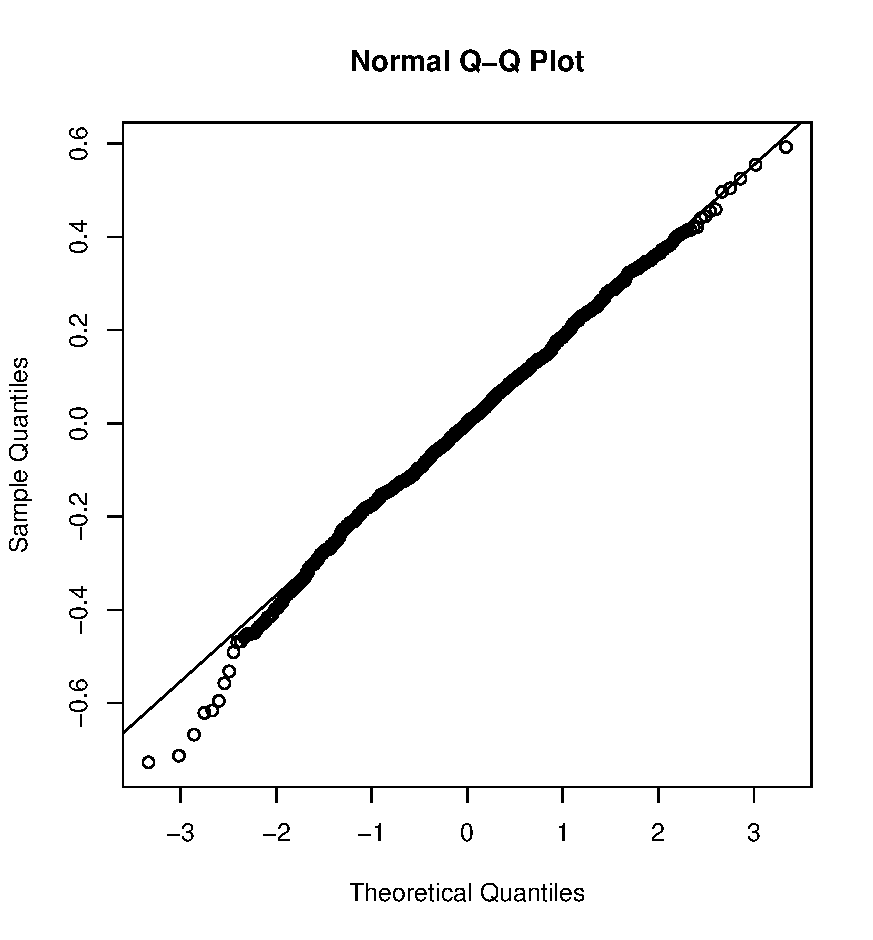
\includegraphics[width = \textwidth]{figures/denheryesyeysyes.pdf}
    \caption{Testing for normality}
    \label{fig:F_chp_resu}
\end{subfigure}%
\begin{subfigure}[b]{0.5\textwidth}
\centering
    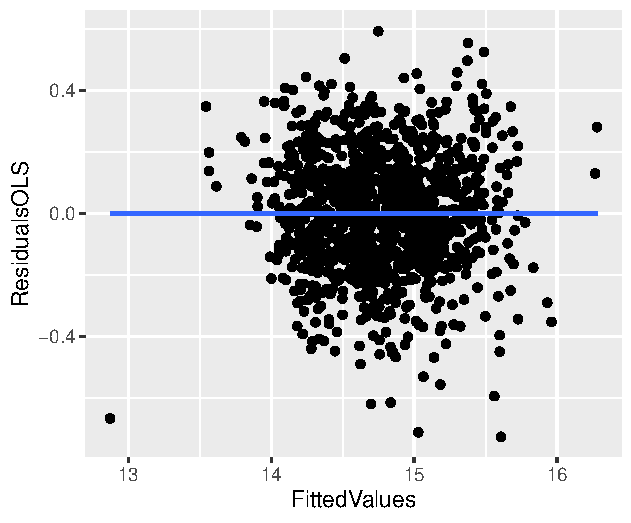
\includegraphics[width = \textwidth]{figures/RplotDenHerHejhej.pdf}
    \caption{Testing for \hetero}
    \label{fig:F_chp_hetero}
\end{subfigure}
\caption{Plots of the residuals in the linear regression performed for the model for Copenhagen determined by the F-test.}
\label{fig:F_cph_plot}
\end{figure}

From the QQ-plot in figure \ref{fig:F_chp_resu} it is seen that the residuals follow a normal distribution quite closely, wherefore we conclude the residuals satisfy assumption \ref{as:normality_of_errors}. 
From  figure \ref{fig:F_chp_hetero} we see that the residuals are randomly distributed. 
With this in mind we conclude that even though the residuals are not theoretically homoskedastic we consider for all practical purposes that the assumption is satisfied.
We therefore conclude the amount of heteroskedasticity is without substantial meaning in our tests and thus our earlier theory regarding the BLUE and hypotheses testing is valid. 
The test for heteroskedasticity has been conducted for all models found with $F$-tests and cross-validation, and has found that heteroskedasticity is theoretically present in all models but graphically that the amount of heteroskedasticity is not a concern thus we will still consider OLS as the BLUE and that hypothesis testing are still valid. 
To support this statement we will conduct both the hetero robust and usual $t$- and $F$-test for these models.

\subsubsection{Application of Heteroskedastic Robust \textit{t}-test}

In this section we wish to compare the $t$-test calculated in section \ref{ex:ttest} with the hetero robust $t$-test. 
\begin{lstlisting}
#The linear regression model, 
#which is the same as in the section with an application of t-test. 
lin_reg <-lm(log(price)~log(size),data = Copenhagen)

#Values which are the same as in the section with the application of the t-test. 
x <- c(rep(1, n), log(Copenhagen$size))
X <- matrix(data = x, nrow = n)
beta_hat <- 0.96832
beta_null <- 0
df <- n - (k + 1)

#Calculating the remaining contents of the variance formula. 
residuals <- residuals(lin_reg)
diag_residuals <- diag(lin_reg$residuals)

#Formula for variance
variance_HC <- 
    solve(t(X) %*% X) %*% t(X) %*% diag_residuals^2 %*% X %*% solve(t(X) %*% X)
    
#Square root is taken to obtain standard error
std_error_HC <- sqrt(variance_HC[2,2])

#We calculate the t-statistic
t_stat_HC <- (beta_hat-beta_null)/std_error_HC; t_stat_HC
[1] 49.05654

#p-value
p_val_HC <- pt(t_stat_HC, df = df, lower.tail = FALSE)*2; p_val_HC
[1] 4.016368e-287
\end{lstlisting}

In section \ref{ex:ttest} the $t$-value was $57.59$ and the $p$-value was $0$. 
The $t$-statistic is a bit lower with hetero robust $t$-test but the $p$-values are very similar and reach the same conclusion about our null hypothesis. 

\subsubsection{Application of Robust Heteroskedastic \textit{F}-test}
Next we will compare the hetero robust $F$-test with section \ref{sec:app_F_test}. 
\begin{lstlisting}
#First we filter the data to only contain the data for Copenhagen. 
cities.data.cph <- filter(cities.data, city == 'Copenhagen'); cities.data.cph

#The models
lin.reg1 <- lm(log(price) ~ log(size) + cond + balcony + 
    year.sale, data = cities.data)
lin.reg0 <- lm(log(price) ~ log(size) + year.sale, data = cities.data)

#Degrees of freedom and number of observations. 
df_mod1 <- n - length(lin.reg1$coefficients)
df_mod0 <- n - length(lin.reg0$coefficients)
n <- length(log(cities.data$price))
q <- df_mod0 - df_mod1

#The estimated betas found from regressing on lin.reg1
betahat <- matrix(c(10.05270, 0.99373, -0.02849, -0.16511,
    0.04648, 0.02673, 0.26932), nrow = 7, ncol = 1)

#Matrix R which checks restrictions on beta estimates for 
#cond.middel, cond.high and balcony. 
R <- matrix(c(0,0,0,0,0,0,1,0,0,0,1,0,0,0,1,0,0,0), nrow = 3, ncol = 7)

#The restrictions in R is set equal to a null vector r, 
#to see if the variables are insignificant. 
r <- matrix(c(0,0,0), nrow = 3, ncol = 1)

#The columns of X. 
intercept <- rep(1, length(cities.data.cph$price))
log.size <- log(cities.data.cph$size)
cond.medium <- ifelse(cities.data.cph$cond == 'Medium', 1, 0)
cond.high <- ifelse(cities.data.cph$cond == 'High', 1, 0)
balcony <- cities.data.cph$balcony
year.sale.crisis <- ifelse(cities.data.cph$year.sale == 'crisis', 1, 0)
year.sale.post.crisis <-
    ifelse(cities.data.cph$year.sale == 'post.crisis', 1, 0)
X <- cbind(rep(1, n), log.size, cond.medium, cond.high, 
    balcony, year.sale.crisis, year.sale.post.crisis)

#s^2 is calculated. 
resi <- rbind(lin.reg1$residuals) %*% cbind(lin.reg1$residuals)
s2 <- (  (resi)  )/(n-6-1)

#The values are insterted into the formula
#for the heteroskedastic robust F-test. 
F_wald_test <- ((   (  t(R %*% betahat - r) %*% 
    solve(R %*% solve(t(X) %*% X) %*% t(R) ) %*% 
    (R %*% betahat - r))/(q)))/s2

#The F-value and p-value from the test. 
F_value <- 22.93383
p_value_wald <- pf(q = F_wald_test, df1 = df_mod0, 
    df2 = df_mod1, lower.tail = F); 
p_value_wald
[1]    0
\end{lstlisting}

Recall the application of the $F$-test from \ref{sec:app_F_test}, where the $F$-statistic was $43.67925$ and the $p$-value was smaller than $2.2e^-16$. The $F$-statistic is much lower with the hetero robust $F$-test but the $p$-values from both tests reach the same conclusion on the null hypothesis. 




    











% The Wald statistical test on a single parameter with $\mathcal{H}_0 : \betahat_j = 0$ is given as
% \begin{align*}
%     Z_i = \dfrac{\betahat_j}{\sqrt{\Var(\betahat_j)}}
% \end{align*}
% For large $n$ the distribution is approximately $N(0,1)$. The variance $\Var(\betahat_j)$ depends on the error term and thus are invalid in the presence of heteroskedasticity.
% If we wish to test the joint significance of multiple coefficient the Wald's Statistics the test is given as
% \begin{align*}
%     W = (\mathbb{X}\betahat - \mathbf{y})^\top [\mathbf{X} \Var(\betahat) \mathbf{X}^\top](\mathbf{X}\betahat - \mathbf{y})
% \end{align*}
% This Wald Statistic is an F-statistics if it is divided with $q$. Thus o


% The asymptotic distribution of the Wald-Statistic can be used to test multiple hypotheses.




















\section{Prediction}\label{sec:prediction}
It is often wanted to deduce information about future observations based on the existing fitted regression model. 
In our case this is predicting future apartment prices. 
Due to this, prediction intervals are introduced as an estimate of an interval that contains a future observation with a certain probability with respect to already observed data.

In this section we assume a general linear model $\textbf{Y}\sim N_n(\textbf{X}\betabold, \sigma^2 \textbf{I}_n)$, where the design matrix $\textbf{X}$ has full rank $(k+1)<n$, and where $\betabold \in \mathbb{R}^{(k+1)}$ and $\sigma^2>0$ are unknown. 
Suppose an observed realization of $\textbf{Y}=\textbf{y}$ and a future random variable $Y_{n+1}$ where
\begin{align*}
    Y_{n+1}\sim N(\textbf{x}_{n+1}\betabold,\sigma^2)
\end{align*}
are independent of $\textbf{Y}$ and where $\textbf{X}$ and $\textbf{x}_{n+1}\in\mathbb{R}^{(k+1)}$ are known. 
The natural prediction value for $\textbf{Y}_{n+1}$ is the MLE for its mean, that is c.f. \eqref{eq:betahat_y}
\begin{align*}
    \hat{Y}_{n+1}(\textbf{y})=\textbf{x}_{n+1}\hat{\betabold}(\textbf{y}).
\end{align*}
The corresponding random variable $\hat{Y}_{n+1}(\textbf{Y})$ is called the predictor for $Y_{n+1}$. 
We now want to determine the variability of $Y_{n+1}$.

Given that $\hat{\betabold} \sim N_k(\betabold,\sigma^2(\textbf{X}^\top\textbf{X})^{-1})$ then $\hat{Y}_{n+1}(\textbf{Y})\sim N(\textbf{x}_{n+1}\betabold,\sigma^2\textbf{x}_{n+1}(\textbf{X}^\top\textbf{X})^{-1}\textbf{x}^\top_{n+1})$ and $Y_{n+1}\sim N(\textbf{x}_{n+1}\betabold,\sigma^2)$ are independent.
Thus we obtain uncertainty of the estimate
\begin{align*}
    Y_{n+1}-\hat{Y}_{n+1} \sim N(0, \sigma^2(1+\textbf{x}_{n+1}(\textbf{X}^\top\textbf{X})^{-1}x_{n+1}^\top)).
\end{align*}

Further the variance estimator
\begin{align*}
    s^2(\textbf{Y})=\frac{\|\textbf{Y} - \textbf{X}( \textbf{X}^\top\textbf{X} )^{-1}\textbf{X}^\top\textbf{Y}\|^2}{n-(k+1)} \sim \frac{\chi^2(n-(k+1))}{(n-(k+1))}
\end{align*}
is independent of $Y_{n+1}-\hat{Y}_{n+1}(\textbf{Y})$ because of independence of data.
From this we define
\begin{align*}
    T=\frac{Y_{n+1}-\hat{Y}_{n+1}(\textbf{Y})}{\sqrt{s^2(\textbf{Y})(1+\textbf{x}_{n+1}(\textbf{X}^\top\textbf{X})^{-1}\textbf{x}^\top_{n+1})}}
\end{align*}
and recall the proof of theorem \ref{th:t_distribution} from which we concluded that
\begin{align*}
    T=\frac{Y_{n+1}-\hat{Y}_{n+1}(\textbf{Y})/\sqrt{\sigma^2(1+\textbf{x}_{n+1}(\textbf{X}^\top\textbf{X})^{-1}\textbf{x}^\top_{n+1})}}{\sqrt{s^2(\textbf{Y})/\sigma^2}} \sim t(n-(k+1)).
\end{align*}
From this it entailes for $0<\alpha<1$ with probability $(1-\alpha)$ that $Y_{n+1}$ is contained in the interval with limits
\begin{align*}
    \hat{Y}_{n+1}(\textbf{Y})\pm t_{\alpha/2}(n-(k+1))\sqrt{s^2(\textbf{Y})(1+\textbf{x}_{n+1}(\textbf{X}^\top\textbf{X})^{-1}\textbf{x}^\top_{n+1})}
\end{align*}
and by substituting $\textbf{Y}$ with the observation $\textbf{y}$ we obtain the $(1-\alpha)\%$-prediction interval for $Y_{n+1}$
\begin{align} \label{eq:predict_interval}
    \hat{Y}_{n+1}(\textbf{y})\pm t_{\alpha/2}(n-(k+1))\sqrt{s^2(\textbf{y})(1+\textbf{x}_{n+1}(\textbf{X}^\top\textbf{X})^{-1}\textbf{x}^\top_{n+1})}
\end{align}
This is the interval of which we expect future observations to be with probability $(1-\alpha)$ given that our assumptions are correct.
If we compare the $(1-\alpha)\%$-prediction interval in \eqref{eq:predict_interval} to the $(1-\alpha)\%$-confidence interval in \eqref{eq:t_statistic} it is clear that the $(1-\alpha)\%$-prediction interval is the largest.
This is caused by prediction intervals contain both the uncertainty in estimating the ``true'' mean and the the random variation of the individual values.

\subsection{Application of Prediction}\label{subsec:app_of_prediction}
Now that we have found models based on both cross-validation and $F$-tests, we can use these models to predict 2016 apartment prices in order to validate the predictive performance of said models.
In figure \ref{fig:predictive_performance} we can see how the predictive performance differs for the two methods.
For Copenhagen the model obtained from cross-validation performs better than the model obtained using $F$-test.
However for Odense the opposite is true, here the $F$-test model performs significantly better than the one obtained from cross-validation.
As it is also evident on the plot the models found from the two methods in Aarhus and Aalborg are identical, as these have the same RMSE.
\begin{figure}[H]
    \centering
    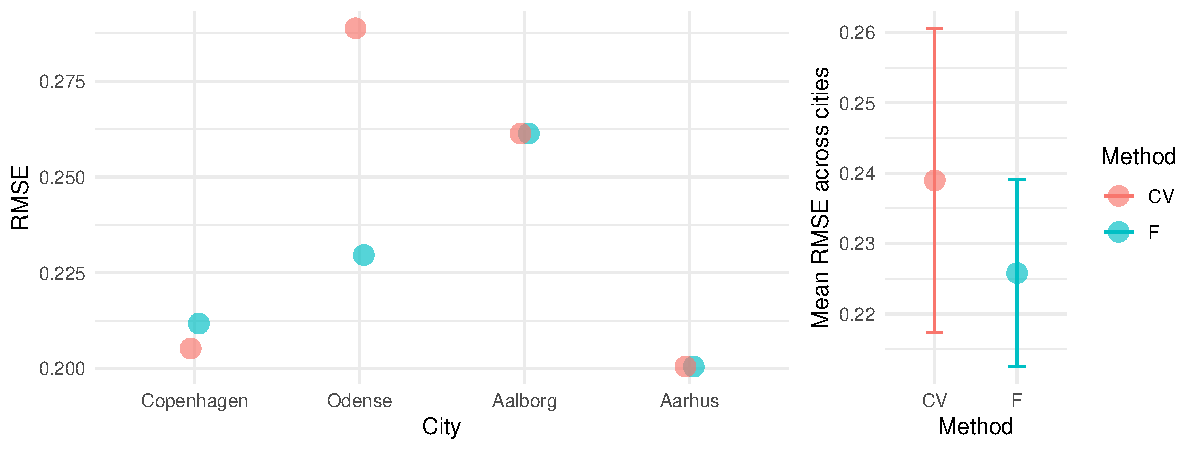
\includegraphics[width = .9\textwidth]{figures/Data_introduction/predictive_performance.pdf}
    \caption{Predicitive performance for the four cities.}
    \label{fig:predictive_performance}
\end{figure}
In table \ref{tbl:predictive_performance} the mean RMSE for the two methods across the four cities is presented.
We observe some difference between the two methods.
\begin{table}[H]
    \centering
    \begin{tabular}{lrr}
        \toprule
        \textbf{Method} & \textbf{Mean RMSE} & \textbf{RMSE std.$\!$ error}\\
        \midrule
        CV & 0.239 & 0.0216\\
        F & 0.226 & 0.0133\\
        \bottomrule
    \end{tabular}
    \caption{Mean RMSE and the associated standard error across the four cities.}
    \label{tbl:predictive_performance}
\end{table}
In our case we conclude that using $F$-test we get better slightly better predictive performance across the four cities.

\subsubsection{Prediction Interval}
We will now treat the observations from 2016 as our future observations $Y_{n+1}, \ldots, Y_{n+200}$, in order to determine if they fall inside the prediction interval.

The prediction interval is obtained using \eqref{eq:predict_interval}, or equivalently in R as
\begin{lstlisting}
    predict.int <- predict(linreg1, cities.data.2016, interval="predict")
\end{lstlisting}
Where \texttt{linreg1} is the model found in section \ref{sec:Ftest} depending on the city. 

The number of observations within this interval, for each of the models, is summed up in table \ref{tbl:Within_prediction_interval}. 
\begin{table}[H]
    \centering
    \begin{tabular}{l|rrrr}
        \toprule
        \textbf{Description} & \textbf{Copenhagen} & \textbf{Aarhus} & \textbf{Odense} & \textbf{Aalborg}\\
        \midrule
        Observations in 2016 & 108              & 46         & 27            & 19 \\
        Within Confidence Interval & 102           & 45            & 26        & 17 \\
        \% Within Confidence Interval & 94    & 98  & 96  & 89 \\
        \bottomrule
    \end{tabular}
    \caption{Observations from 2016 that fall within the prediction intervals.}
    \label{tbl:Within_prediction_interval}
\end{table}
Except for Aalborg, this seems to align well with the assumption of 95\% of observations falling within the prediction interval.
As expected from section \ref{sub:residuals} the model for Aalborg indeed has inferior predictive performance. 
While this does not verify the model, it is an indication that it can be used for prediction of future apartment prices.
These prediction intervals were found using the $F$-models, but we could just as well have used the CV-models. 
Since the models are so similar the number of observations within the prediction interval is unchanged and thus will not be repeated, see table \ref{tbl:Within_prediction_interval}.

For the dependent variable to be meaningful, it needs to be converted from $\log(price)$ back to $price$. 
This is calculated by
\begin{align*}
    price = e^{\log(price) + \frac{1}{2} s^2},
\end{align*}
since $price$ has a log-normal distribution.  
The fitted values and their prediction intervals is plotted in figure \ref{fig:predictive_intervals_observations_fitted}, along with the actual observations. 
\begin{figure}[H]
    \centering
    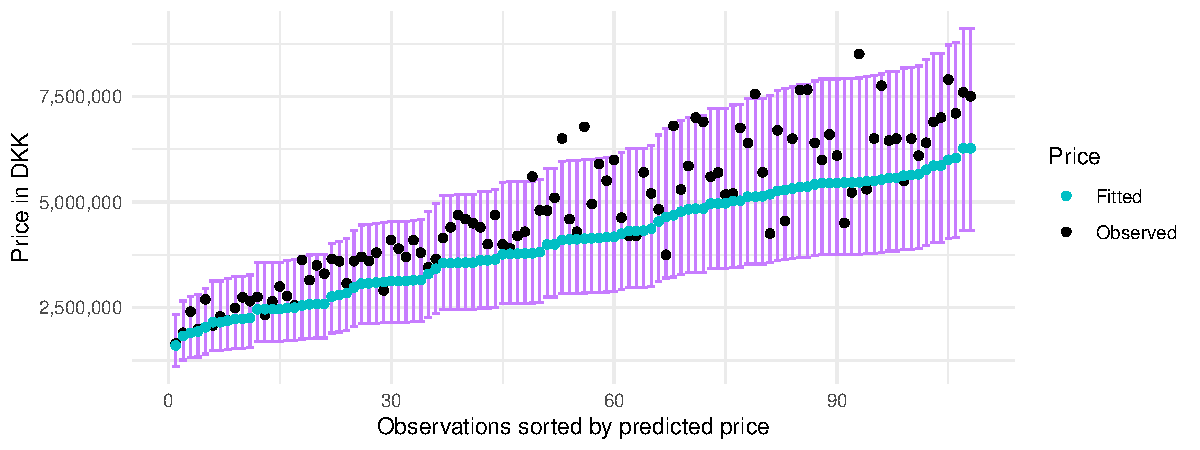
\includegraphics[width = .8\textwidth]{figures/prediction_interval.pdf}
    \caption{2016 observations for Copenhagen, fitted values and their prediction intervals.}
    \label{fig:predictive_intervals_observations_fitted}
\end{figure}
The model consistently underpredicts the price of apartments, but about 95\% still fall within the prediction intervals. 
The reason for this is likely a lacking parameter or a faulty interpretation of one or multiple of the parameters included in the model. 
This could for example be the dummy variables for year.sale. 
Here the $post.crisis$ coefficient may not be representative for the general level of house pricing in 2016.



% \begin{figure}[H]
%     \centering
%     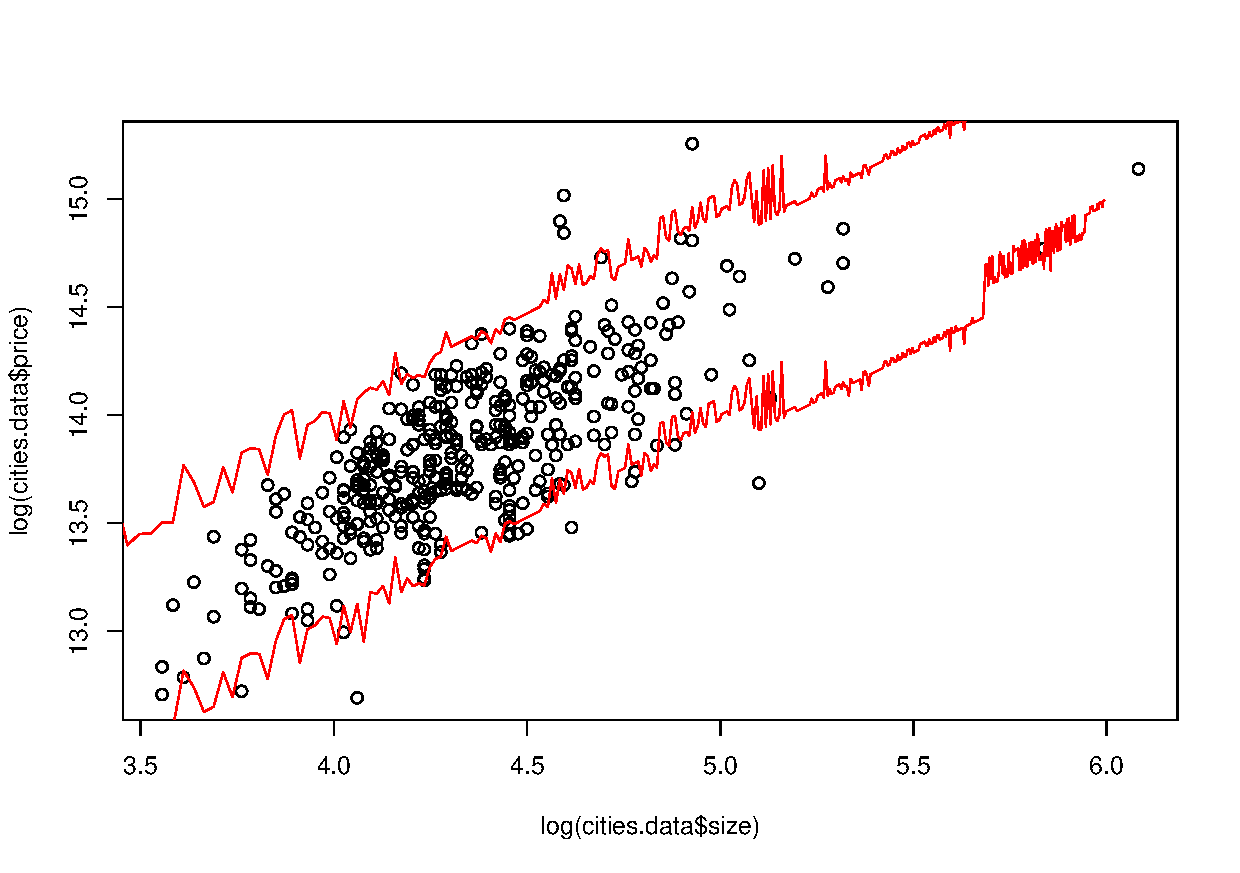
\includegraphics[width = .6\textwidth]{figures/ConfidenceInterval2015.pdf}
%     \caption{Observation for 2004-2015 and prediction interval}
%     \label{fig:confidence_intervals2015}
% \end{figure}



\section{Error Diagnostics}
In this section prediction errors of the obtained models from $F$-test and cross-validation are investigated. The investigation covers both included and previously excluded variables. We want to clarify if the errors are systematic in any way.

In this section we focus on the errors obtained from the model for Copenhagen from cross-validation.
In figure \ref{fig:error_cont} the prediction errors of the model and the continuous predictors are plotted in scatterplots. 
Overall, the model seems to underpredict the prices on the 2016 data. 
This indicates, that the prices were generally increased in the year 2016 compared to the weighted average of the remaining years in $post.crisis$. 
The prediction errors, $pred$, seems to be heteroskedastic as the variance increases with the size of the predicted values. 
This might indicates some unexplained structure in the errors or could just be caused by randomness. 
$selling.period$ and $year.construct$, which were excluded from the model, only have a small negative slope and therefore would not contribute with much explanatory value for the 2016 data.
The errors of $size$ appear heteroskedastic as the variance peeks at the middle. 
\begin{figure}[H]
        \centering
      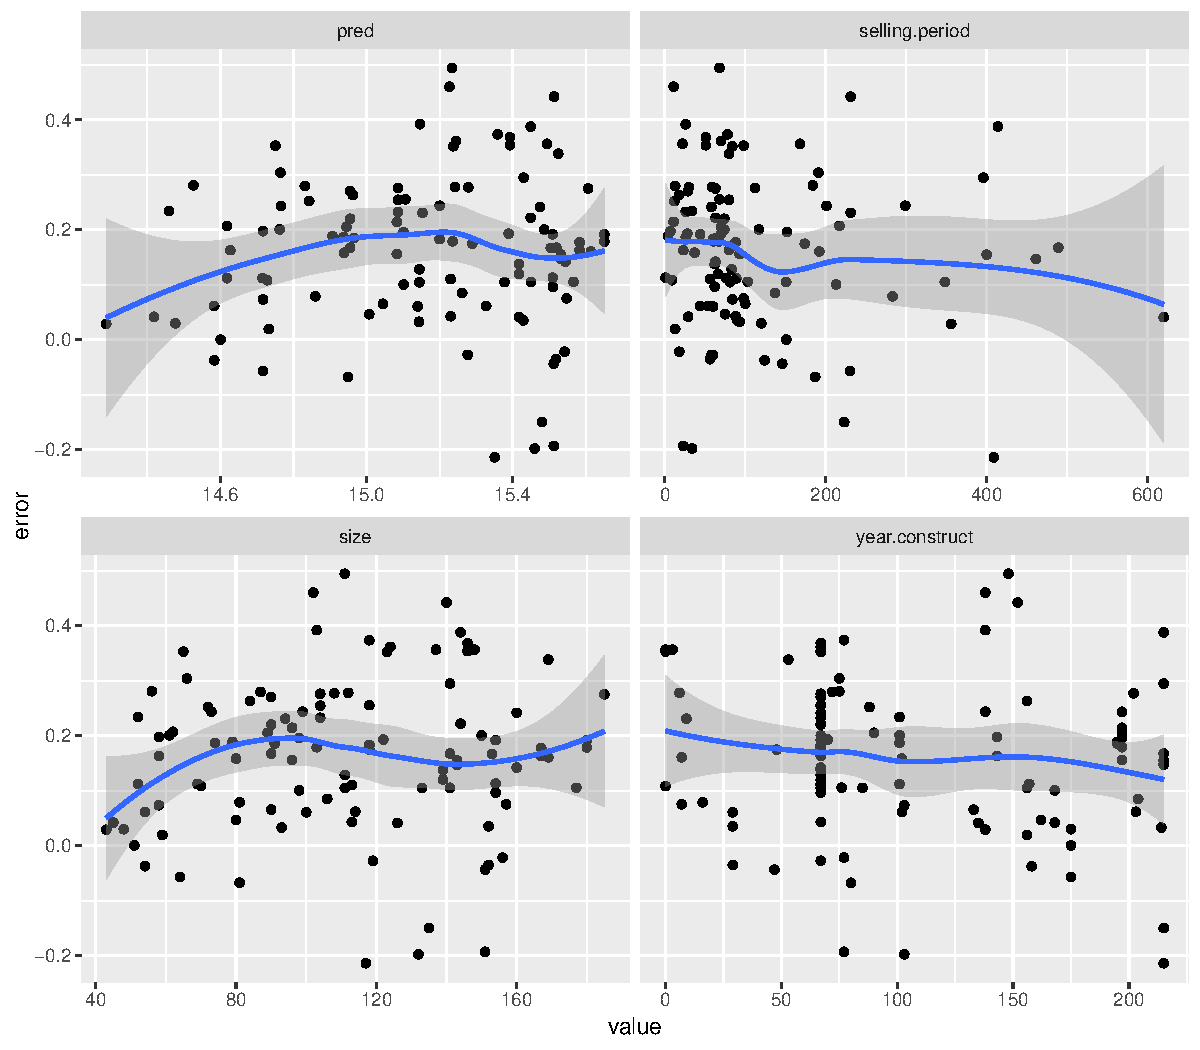
\includegraphics[width = 0.7 \textwidth]{figures/Nanna/errors_continuous.pdf}
      \caption{Scatterplots of the prediction errors calculated from the model found for Copenhagen. }
      \label{fig:error_cont}
\end{figure}
In figure \ref{fig:error_factor} are boxplots of the factor variables. 
Again, an overall conclusion is, that the model underpredicts the data from 2016.
For $balcony$ the median is almost the same for each of the two values.
However, the distribution of the errors of apartments with $balcony$ is skewed and has potential outliers. 
For $cond$ the errors decreases with the state of the condition of the apartments.
The value ``Low'' is affected by a small number of observations. 
\textit{renovation}, which was excluded from the model, has almost the same median error for each of its two values. 
\begin{figure}[H]
        \centering
      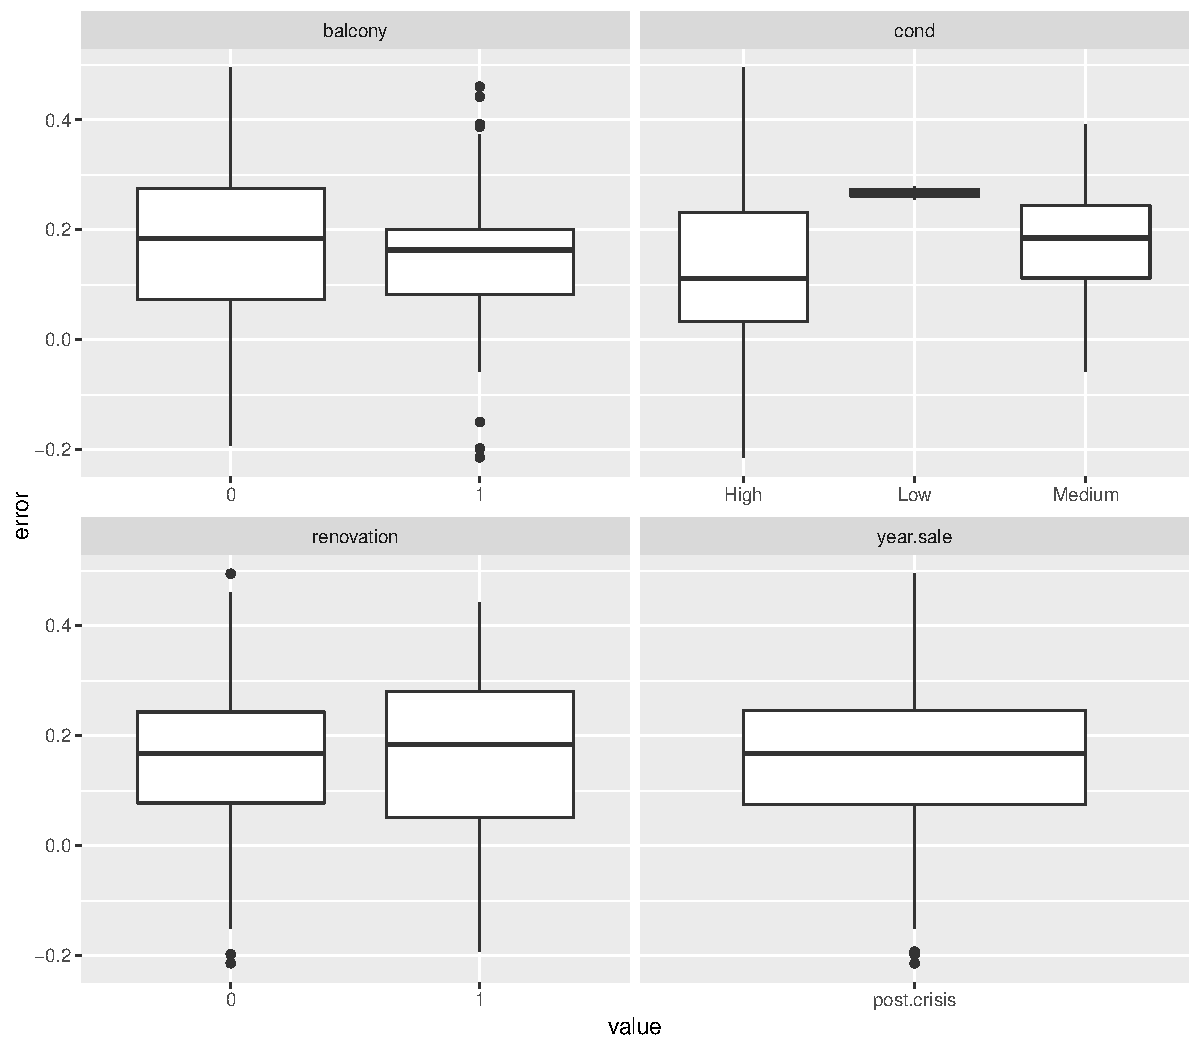
\includegraphics[width = 0.7 \textwidth]{figures/Nanna/errors_factors.pdf}
      \caption{Boxplots of the prediction errors calculated from the model found for Copenhagen.}
      \label{fig:error_factor}
\end{figure}
A lot of the same conclusions are drawn about the remaining models and all the models underpredict the prices due to the majority of the errors being positive.
The models obtained from F-test and cross-validation only differs for Aarhus and Odense, but these have very similar prediction errors.
All the models underpredict the prices due to the majority of the errors being positive.
$renovation$ seems to be able to add some explanatory value to the 2016 data for the models for Aarhus and Odense.  
The relation between prediction errors and $cond$ is a little different between cities. 

From the error diagnostic the main conclusion is that the models underpredict.
This is to a great extent caused by the omission of the increasing trend in prices in the $post.crisis$ category. 
\newpage
\section*{Mini-project}
We have $Y_1,...,Y_n$ as underlying random variables for observations/data/responses $y_1,...,y_n$.
Specifically, we let $Y_1,...,Y_n$ be independent normally distributed random with variance $1$, and let $\mu_i= E[Y_i]$ be the mean of $Y_i, i= 1,...,n$.
Furthermore, we let $x_1,...,x_n$ be given numbers; when the distribution of $(Y_1,...,Y_n)$ depends on $(x_1,...,x_n)$ we also call $(Y_1,...,Y_n)$ the dependent variables and $(x_1,...,x_n)$ the explanatory variables (or the independent variables, though this may be misleading terminology).

\subsection*{Exercise 2.1 The First Model}

Assume that
\begin{align*}
    \mu_i = \alpha, \quad i = 1, \ldots,n
\end{align*}
where $\alpha$ is an unknown real parameter. 

\begin{enumerate}
    \item Specify the log likelihood function, the score function, the observed information matrix and the Fisher information matrix
\end{enumerate}

\subsubsection{Log likelihood function}
First we find the likehood function, which here is the product of standard normal distribution. The pdf is 

\begin{align*}
   L(Y;\mu) &= \prod_{i=1}^n \left[ \frac{1}{\sigma \sqrt{2 \pi}}exp\left(-\frac{(y_i -\mu_i)^2}{2 \sigma^2}\right) \right]\\
\end{align*}

Now we take log to the above equation to obtain the log likelihood function

\begin{align*}
   \ell(Y;\alpha) &= log \left( \prod_{i=1}^n \left[ \frac{1}{\sigma \sqrt{2 \pi}}exp\left(-\frac{(y_i -\mu_i)^2}{2 \sigma^2}\right) \right] \right)\\
   &= \sum_{i = 1}^n \left[ log\left( \frac{1}{\sigma \sqrt{2 \pi}}exp\left[-\frac{(y_i - \mu_i)^2}{2 \sigma^2}\right] \right) \right]\\
   &= \sum_{i = 1}^n \left[ log(1) - log(\sqrt{2 \pi}) - \frac{(y_i - \alpha)^2}{2} \right]\\
   &= \sum_{i = 1}^n \left[- log\left( \sqrt{2 \pi}\right) - \left(\frac{y_i^2 + \alpha^2 - 2y_i\alpha}{2}\right) \right]\\
   &= \sum_{i = 1}^n \left[y_i \alpha - log\left( \sqrt{2 \pi}\right) - \left( \frac{y_i^2 + \alpha^2}{2} \right) \right]
\end{align*}

\subsubsection{Score function}

The score function is the log likelihood function differentiated with respect to its parameter, thus

\begin{align*}
    S\left( Y; \alpha \right) &= \ell'(Y; \alpha)\\
    &= \sum_{i=1}^n \left[ y_i + 0 - \alpha \right]\\
    &= \sum_{i=1}^n \left[ y_i - \alpha \right].
\end{align*}

This is the score function. 

\subsubsection{Observed information}

We now find the observed information, which is the score function differentiated and taken minus to

\begin{align*}
    j\left( Y; \alpha \right) &= - S\left(Y; \alpha \right)\\
    &=  - \left( \sum_{i = 1}^n -1\right) = n.
\end{align*}

\subsubsection{Fisher information matrix}

The Fisher information matrix is the expected value of observed information

\begin{align*}
    i\left(\alpha \right) &= E\left[j(Y;\alpha)\right]\\
    &= n.
\end{align*}

\begin{enumerate}[resume]
    \item  Find the MLE $\hat{\alpha}$.
\end{enumerate}

The MLE is defined as

\begin{align*}
    L(\hat{Y}; \alpha) &= sup L(Y; \alpha)
\end{align*}

and it is found by setting the score function equal to $0$

\begin{align*}
    S\left(Y; \alpha \right) &= 0\\
    \sum_{i=1}^n \left[y_i - \alpha \right]&= 0\\
    n\alpha &= \sum_{i=1}^n y_i\\
    \hat{\alpha} &= \frac{1}{n} \sum_{i=1}^n y_i \\
    \hat{\alpha} &= \bar{y},
\end{align*}
where $\bar{y}$ is the mean of the observed values $y_i$ for $i = 1, \ldots n$.

\begin{enumerate}[resume]
    \item  Specify the asymptotic distribution of $\hat{\alpha}\xrightarrow \infty$. Use this to obtain an approximate $95\%$-confidence interval for $\alpha$.
\end{enumerate}

\begin{theorem}[Distribution of the ML estimator]\label{th:distribution_ml_estimator}
Let $E = \{\mathbf{y} \ : \ \text{the MLE } \hat{\theta}(\mathbf{y}) \text{ exists}\}$. 
If $A$ is a $k \times k$ matrix, $A^{1/2}$ denotes the $k \times k$ matrix such that $A = A^{1/2}\left( A^{1/2} \right)^T$.
Let $\rightarrow^\mathcal{D}$ denote convergence in distribution, $\mathbf{1}[\cdot]$ the indicator function and $I_k$ the $k \times k$ identity matrix.
Then under regularity conditions, if $\mathbf{Y} \sim f(\cdot;\theta)$ then as $n \rightarrow \infty$ we have that
\begin{enumerate}
    \item $P_\theta(Y \in E) \rightarrow 1$
    \item for any $\varepsilon > 0: \ P_\theta(Y \in E, \ \|\hat{\theta} - \theta\| \leq 1) \rightarrow 1$
    \item $1[\mathbf{y} \in E] i(\hat{\theta})^{1/2}(\hat{\theta} - \theta) \rightarrow^\mathcal{D} N_k(0, I_k)$ and $1[\mathbf{y} \in E] j(\hat{\theta})^{1/2}(\hat{\theta} - \theta) \rightarrow^\mathcal{D} N_k(0, I_k)$
    \item $1[\mathbf{y} \in E] i(\theta)^{1/2}(\hat{\theta} - \theta) \rightarrow^\mathcal{D} N_k(0, I_k)$
\end{enumerate}
\end{theorem}

% \begin{center}
% -----
% \textbf{Udledning mangler}
% -----
% \end{center}

By theorem \ref{th:distribution_ml_estimator} the asymptotic distribution of the ML estimator is given by
\begin{align*}
    \hat{\theta} \rightarrow^\mathcal{D} N\left( \theta, \boldsymbol{i}(\theta)^{-1} \right)
\end{align*}

Since $\alpha$ is one-dimensional, $k=1$, and for $0\leq a \leq 0.5$ we have the approximate $(1-a)$-confidence interval
\begin{align*}
\left[ \hat{\alpha}(\mathbf{y}) + \Phi_{a/2} \sqrt{D\left( \hat{\alpha}\left(\mathbf{y}\right)\right)}, \hat{\alpha}(\mathbf{y}) + \Phi_{1 - a/2} \sqrt{D\left( \hat{\alpha}\left(\mathbf{y}\right)\right)} \right],
\end{align*}
where $D\left(\hat{\alpha}(\mathbf{y})\right) = j\left(\hat{\alpha}(\mathbf{y})\right)^{-1}$.
For $a=0.05$ we have the approximate $95\%$-confidence interval for $\alpha$:
\begin{align*}
\left[ \bar{y} - \frac{1.96}{\sqrt{n}}, \bar{y} + \frac{1.96}{\sqrt{n}} \right]    
\end{align*}

\subsection*{Exercise 2.2 The second model}

Assume that
\begin{align*}
    \mu_i=\alpha \beta^{x_i}, \quad i=1,\ldots, n
\end{align*}
where $\alpha$ and $\beta$ are unknown real parameters. Then $x_1, \ldots,x_n$ are called explanatory variables. 

\begin{enumerate}
    \item Specify the log likelihood function, the score function, the observed information matrix and the Fisher information matrix
\end{enumerate}

\textbf{Log likelihood function}
In order to find the log likelihood function, we first find the likelihood function

\begin{align*}
   L(Y;\mu) &= \prod_{i=1}^n \frac{1}{\sigma \sqrt{2 \pi}}exp\left[-\frac{(y_i -\mu)^2}{2 \sigma^2}\right].\\
\end{align*}

Now we take log of the above equation, to obtain the loglikelihood

\begin{align*}
   \ell(Y;\alpha, \beta) &= log \left( \prod_{i=1}^n \frac{1}{\sigma \sqrt{2 \pi}}exp\left[-\frac{(y_i -\mu)^2}{2 \sigma^2}\right] \right)\\
   &= \sum_{i = 1}^n \left[ y_i \alpha \beta^{x_i} - log\left( \sqrt{2 \pi}\right) - \left( \frac{y_i^2 + (\alpha \beta^{x_i})^2}{2} \right) \right]\\
   &=\sum_{i = 1}^n \left[ y_i \alpha \beta^{x_i} - log\left( \sqrt{2 \pi}\right) - \left( \frac{y_i^2 + (\alpha^2 \beta^{2x_i})}{2} \right) \right].\\
\end{align*}

\textbf{Score function}

\begin{align*}
    S\left( Y; \alpha, \beta \right) = \begin{bmatrix} S(Y;\alpha) \\ S(Y; \beta) \end{bmatrix} = \begin{bmatrix} \sum_{i=1}^n y_i \beta^{x_i} - \alpha\beta^{2x_i} \\ \sum_{i = 1}^n y_i\alpha x_i \beta^{x_i - 1} - \alpha^2 x_i \beta^{2x_i - 1} \end{bmatrix}.
\end{align*}

Here the Score function is a vector, because it has more than one variable. 

\subsubsection{Observed information}

We now find the observed information as before, but because of the parameters, it is now a matrix

\begin{align*}
    j\left( Y; \alpha ,\beta \right) = \begin{bmatrix} 
    \sum_{i = 1}^n \beta^{2x_i} 
    &
    \sum_{i = 1}^n 2\alpha x_i \beta^{2x_i - 1} - y_ix_i\beta^{x_i - 1}
    \\
    \sum_{i = 1}^n 2\alpha x_i \beta^{2x_i - 1} - y_ix_i\beta^{x_i - 1} 
    &
    \sum_{i = 1}^n \alpha^2(2x_i - 1)x_i\beta^{2x_i - 2} - y_i \alpha x_i(x_i - 1) \beta^{x_i - 2}
    \end{bmatrix}.
\end{align*}

\subsubsection{Fisher information matrix}

The Fisher information matrix is the expected value of observed information

\begin{align*}
    i\left(\alpha \beta^{x_i} \right) &= E\left[j(Y;\alpha ,\beta)\right]\\
    &= \begin{bmatrix} 
    \sum_{i = 1}^n \beta^{2x_i} 
    &
    \sum_{i = 1}^n 2\alpha x_i \beta^{2x_i - 1} - \alpha\beta^{x_i}x_i\beta^{x_i - 1}
    \\
    \sum_{i = 1}^n 2\alpha x_i \beta^{2x_i - 1} - \alpha\beta^{x_i}x_i\beta^{x_i - 1}
    &
    \sum_{i = 1}^n \alpha^2(2x_i - 1)x_i\beta^{2x_i - 2} - \alpha \beta^{x_i} \alpha x_i(x_i - 1) \beta^{x_i - 2}
    \end{bmatrix} \\
    &= \begin{bmatrix} 
    \sum_{i = 1}^n \beta^{2x_i}  
    &
     \sum_{i = 1}^n 2\alpha x_i \beta^{2x_i - 1} - \alpha\beta^{2x_i-1}x_i
    \\
    \sum_{i = 1}^n 2\alpha x_i \beta^{2x_i - 1} - \alpha\beta^{2x_i-1}x_i
    &
    \sum_{i = 1}^n \alpha^2(2x_i - 1)x_i\beta^{2x_i - 2} - \alpha \beta^{2x_i - 2} \alpha x_i(x_i - 1)
    \end{bmatrix}\\
    &= \begin{bmatrix} 
    \sum_{i = 1}^n \beta^{2x_i}  
    &
     \sum_{i = 1}^n  \alpha\beta^{2x_i-1}x_i
    \\
    \sum_{i = 1}^n  \alpha\beta^{2x_i-1}x_i
    &
    \sum_{i = 1}^n n\alpha^2 x_i^2 \beta^{2x_i - 2}
    \end{bmatrix}.  
\end{align*}

\begin{enumerate}[resume]
    \item Discuss how you will find the MLE in the following cases: 
    \begin{enumerate}[label = (\alph*)]
        \item By using the optim command in R
    \end{enumerate}
The optim function in R takes as input, a vector containing initial values and a objective function.
The function then uses as default the ``Nelder-Mead'' procedure for minimizing the objective function. This is a procedure that uses only the function values and is therefore useful for dealing with non-differentiable functions.

When dealing with differentiable functions the performance of the optim function can be improved as the function can now use other methods such as BFGS. 
This is a method the makes use of the gradient of the objective function.
It can therefore find a minimum of the function in fewer iterations.

As the optim function takes an initial value, the point at which the function terminates will vary depending on the initial value.
For the function given by
\begin{align*}
    f(x,y) = x^2 + y^2
\end{align*}
the initial value makes no difference as the function has only one minimum, namely at $(0,0)$.
Consider instead the function
\begin{align*}
    g(x,y) = sin(x) + cos(y)
\end{align*}
as this function have an indefinite amount of minimums, the minimum returned by the function will depend on the initial value given.
    \begin{enumerate}[label = (\alph*), resume]
        \item First fix $\beta$ and find the MLE of $\alpha$ in term of $\beta$, denoted $\hat{\alpha}(\beta)$, next find the MLE of $\beta$ and hence that of $\alpha$-the likelihood function with $\alpha$ replaced by $\hat{\alpha}(\beta)$ is called the profile likelihood of $\beta$ (or the partially maximized likelihood function) and is denoted $\hat{L}(\beta)$. Specify the Newton-Raphson procedure for finding the MLE of $\beta$ by maximizing $\hat{L}(\beta)$. Will the procedure converge and return that MLE?
    \end{enumerate}
\end{enumerate}


First we find the MLE of $\alpha$ for fixed $\beta$
\begin{align*}
    S\left( Y; \alpha \right) = 0 \\
    \sum_{i=1}^{n} \left[ y_i \beta^{x_i} - \alpha \beta^{2 x_i} = 0 \right] \\
    \sum_{i=1}^{n} y_i \beta^{x_i} = \alpha \sum_{i=1}^{n} \beta^{2 x_i} \\
    \hat{\alpha} = \frac{\sum_{i=1}^{n} y_i \beta^{x_i}}{\sum_{i=1}^{n} \beta^{2x_i}}.
\end{align*}
This estimate is substituted into the score function for $\beta$, to obtain the profile score function of $\beta$, $\hat{S}(\beta)$
\begin{align*}
    S\left( Y; \beta \right) &= \sum_{i=1}^n \left[ y_i x_i \alpha \beta^{x_i - 1} - \alpha^2 x_i \beta^{2 x_i - 1} \right]\\
     &= \sum_{i=1}^n \left[ y_i x_i \beta^{x_i - 1} \left( \dfrac{\sum_{i=1}^n y_i\beta^{x_i}}{\sum_{i=1}^n \beta^{2x_i}}\right) - x_i\beta^{2x_i-1} \left( \dfrac{\sum_{i=1}^n y_i\beta^{x_i}}{\sum_{i=1}^n \beta^{2x_i}}\right)^2 \right].
\end{align*}
Using Taylor expansion and isolating $\beta$ in this expression, we obtain
\begin{align*}
    S_\beta (\beta_i, y_i x) &\approx S_\beta(\beta^*) - i(\beta^*) (\hat{\beta} - \beta^*) = 0 \quad \Rightarrow \quad
    \hat{\beta} = \beta^* + i(\beta^*)^{-1} S_\beta (\beta^*).
\end{align*}
Newton-Raphson finds the roots and thus in our case the maximum. 
The procedure is used to estimate the MLE in cases where $\beta$ cannot be calculated analytically but must be found numerically, therefore the returned MLE is an estimate, that maximizes the log likelihood function.  
As the procedure is sensitive to the initial value given, whether or not it will converge depends.

\begin{enumerate}[resume]
    \item Specify the asymptotic distribution of the MLE $(\hat{\alpha}, \hat{\beta})$ as $n \rightarrow \infty$.
    Use this to obtain approximate 95\%-confidence intervals for $\alpha$ and $\beta$, respectively, and an 95\%-confidence region for $(\alpha, \beta)$
\end{enumerate}

By theorem 2.4 as the sample size tends to infinity the distribution of the ML estimator converges to the normal distribution.
The 95\%-confidence interval for $\alpha$ becomes
\begin{align*}
    \left[ \left( \frac{\sum_{i=1}^n y_i \beta^{x_i}}{\sum_{i=1}^n \beta^{2x_i}}\right) \pm 1.96 \sqrt{D_{11}(Y; \alpha, \beta)} \right]
\end{align*}
where $D = j^{-1}$.
The 95\%-confidence interval for $\beta$ becomes
\begin{align*}
    \left[ \hat{\beta}(y) \pm 1.96 \sqrt{D_{22}(Y; \alpha, \beta)} \right]
\end{align*}
\begin{definition}
Suppose that for a given number $a \in (0,1)$ and for each $y \in \mathcal{Y}$, we have a specified subset $A(y)$ of the parameter space $\Theta^k$ such that
\begin{align*}
    P_\theta(\theta \in A(Y)) = 1 - a \qquad \text{for all } \theta \in \Theta^k.
\end{align*}
Then we call $A(y)$ an (\textit{exact}) $(1 - a)$-\textit{confidence region for} $\theta$.
\end{definition}
One way to define the confidence region is based on the likelihood ratio test.
In our case $A(y)$ becomes
\begin{align*}
    A(y) = \{ (\alpha, \beta) \in \mathbb{R}^2 \ : \ -2 \: \ell_{norm}((\alpha, \beta), Y) \leq \chi^2_{1 - a}(k))\}.
\end{align*}

\begin{enumerate}[resume]
    \item Specify methods for testing the hypothesis $\beta = 1$, i.e., when the model reduces to model 1.
\end{enumerate}
One way to test the hypothesis is using Wilk's likelihood ratio test.

\subsection*{2.3 The third model}
Assume that
\begin{align*}
    \mu_i=\alpha \beta^{x_i}+\gamma, \quad i=1,\vdots n,
\end{align*}
where $\alpha$, $\beta$ and $\gamma$ are unknowwn parameters.
\begin{enumerate}
    \item Specify the log likelihood function, the score function, the observed information matrix and the Fisher information matrix
\end{enumerate}

\subsubsection{Log likelihood function}

In order to find the log likelihood function, we first find the likelihood function

\begin{align*}
   L(Y;\mu) &= \prod_{i=1}^n \left[\frac{1}{\sigma \sqrt{2 \pi}}exp\left(-\frac{(y_i -\mu)^2}{2 \sigma^2}\right) \right].\\
\end{align*}

Now we take log of the above equation, to obtain the log likelihood

\begin{align*}
   \ell(Y;\alpha, \beta, \gamma) &= log \left( \prod_{i=1}^n \left[\frac{1}{\sigma \sqrt{2 \pi}}exp\left(-\frac{(y_i -\mu)^2}{2 \sigma^2}\right) \right] \right)\\
   &= \sum_{i = 1}^n \left[ y_i (\alpha \beta^{x_i}+\gamma) - log\left( \sqrt{2 \pi}\right) - \left( \frac{y_i^2 + (\alpha \beta^{x_i}+\gamma)^2}{2} \right) \right] \\
   &=\sum_{i = 1}^n \left[ y_i \alpha \beta^{x_i} +y_i\gamma - log\left( \sqrt{2 \pi}\right) - \left( \frac{y_i^2 + (\alpha^2 \beta^{2x_i}) + \gamma^2 + 2\alpha\beta^{x_i}\gamma}{2}\right) \right].\\
\end{align*}

\subsection{Score function}

\begin{align*}
    S(y;\alpha,\beta,\gamma)=
    \begin{bmatrix}
    &S(y;\alpha) \\
    &S(y;\beta) \\
    &S(y;\gamma)
    \end{bmatrix} 
\end{align*}

where 

\begin{align*}
    S(y;\alpha) &=\sum_{i=1}^n \left[ y_i\beta^{x_i} - \frac{2\alpha\beta{2x_i}+2\beta^{x_i}\gamma}{2} \right] \\
    &= \sum_{i=1}^n \left[ y_i\beta^{x_i}-\alpha\beta^{2x_1}-\beta^{x_i}\gamma \right]
\end{align*}

\begin{align*}
    S(y;\beta) &= \left[ \sum_{i=1}^n x_i y_i\alpha\beta^{x_i - 1} - \frac{2x_i\alpha^2\beta^{2x_i -1}+2x_i\alpha\beta^{x_i-1}\gamma}{2} \right] \\
    &= \sum_{i=1}^n \left[ x_i y_i\alpha\beta^{x_i-1} - x_i\alpha^2\beta^{2x_i-1} - x_i\alpha\beta^{x_i-1}\gamma \right]
\end{align*}

\begin{align*}
    S(y;\gamma) &= \sum_{i=1}^n \left[ y_i - \frac{2\gamma + 2\alpha\beta^{x_i}}{2} \right]\\
    &= \sum_{i=1}^n \left[ y_i-\gamma-\alpha\beta^{x_i} \right]
\end{align*}

Observed information

\begin{align*}
    &j(Y;\alpha,\beta,\gamma) = \\
    &-\begin{bmatrix}
        \sum_{i=1}^n \beta^{x_i} & \sum_{i=1}^n x_iy_i\beta^{x_i-1}-2x_i\alpha\beta^{2x_i}+x_i\beta^{x_i-1}\gamma & \sum_{i=1}^n \beta^{x_i} \\
       \sum_{i=1}^n x_iy_i\beta^{x_i-1}-2x_i\alpha\beta^{2x_i}+x_i\beta^{x_i-1}\gamma & \sum_{i=1}^n x_i \alpha \beta^{x_i-2}\Big( (x_i - 1) \big( y_i  +  \gamma \big)- (2x_i-1) \alpha \beta^{x_i} \Big) & \sum_{i=1}^n x_i \alpha \beta^{x_i - 1} \\
        \sum_{i=1}^n \beta^{x_i} & \sum_{i=1}^n x_i \alpha \beta^{x_i - 1} & n
    \end{bmatrix}
\end{align*}

Fisher information

\begin{align*}
    &i(Y;\alpha,\beta,\gamma) = \\
    &-\begin{bmatrix}
        \sum_{i=1}^n \beta^{x_i} & \sum_{i=1}^n x_i\alpha\beta^{2x_i-1}+x_i\gamma \beta^{x_i-1}-2x_i\alpha\beta^{2x_i} & \sum_{i=1}^n \beta^{x_i} \\
       \sum_{i=1}^n x_i\alpha\beta^{2x_i-1}+x_i\gamma \beta^{x_i-1}-2x_i\alpha\beta^{2x_i} & \sum_{i=1}^n x_i \alpha \beta^{x_i-2}\Big( 2x_i\gamma - x_i\alpha\beta^{x_i} \Big) & \sum_{i=1}^n x_i \alpha \beta^{x_i - 1} \\
        \sum_{i=1}^n \beta^{x_i} & \sum_{i=1}^n x_i \alpha \beta^{x_i - 1} & n
    \end{bmatrix}
\end{align*}

%Indgang 2,2 \sum_{i=1}^n x_i (x_i - 1) y_i \alpha \beta^{x_i - 2} - x_i (2 x_i -1) \alpha^2 \beta^{2x_i -2} + x_i (x_i -1) \alpha \beta^{x_i -2} \gamma